%% main.tex --- "A Skill's Effect Lives on Its Own Tokens"
%% Submission format: The ACM Web Conference 2027 (WWW '27), research track.
%%
%% The track asks for  \documentclass[sigconf, anonymous, review]{acmart}
%% and caps a long paper at 8 pages of main content plus references and an
%% optional appendix, 12 pages in total, with the first 8 pages self-contained.
%% See https://www2027.thewebconf.org/research-track-papers/
%%
%% Layout of this project
%%   main.tex              this file: preamble, metadata, document skeleton
%%   sections/             main text, one file per section
%%   appendix/             appendices, one file per theme
%%   tables/               tabulars written by the generators in tools/
%%   figures/              figures written by the generators in tools/
%%   skillvector.bib       bibliography
%%
%% Build:  latexmk -pdf main.tex      (or ./build.sh from the repository)

\documentclass[sigconf, anonymous, review]{acmart}

%% ------------------------------------------------------------------ rights
%% Placeholders. Replace with the block the ACM rights form emails you.
\setcopyright{acmlicensed}
\copyrightyear{2027}
\acmYear{2027}
\acmDOI{XXXXXXX.XXXXXXX}
\acmConference[WWW '27]{Proceedings of the ACM Web Conference 2027}%
  {April 2027}{To be announced}
\acmISBN{978-X-XXXX-XXXX-X/27/04}

%% -------------------------------------------------------------- packages
%% acmart already loads graphicx, booktabs, xcolor, hyperref, url and natbib.
\usepackage{amsmath}
% libertine (loaded by acmart) already defines \Bbbk, and amssymb redefines it.
\let\Bbbk\relax
\usepackage{amssymb}
\usepackage{multirow}
\usepackage{tikz}
\usetikzlibrary{arrows.meta,positioning,calc}
\graphicspath{{figures/}}

%% This paper is float-dense: 11 figures and 26 tables, most of them full width.
%% With LaTeX's defaults the appendix queue overflows and floats are dropped
%% without an error, so the page is allowed to be mostly float and float-only
%% pages are allowed to be less than full.
\renewcommand{\topfraction}{0.9}
\renewcommand{\bottomfraction}{0.9}
\renewcommand{\textfraction}{0.06}
\renewcommand{\floatpagefraction}{0.75}
\renewcommand{\dbltopfraction}{0.9}
\renewcommand{\dblfloatpagefraction}{0.7}
\setcounter{topnumber}{4}
\setcounter{bottomnumber}{3}
\setcounter{totalnumber}{6}
\setcounter{dbltopnumber}{4}

%% ---------------------------------------------------------------- macros
% A visible marker for numbers that are not in yet. Must be empty at submission.
\newcommand{\PEND}[1]{\textcolor{red}{[pending: #1]}}
\newcommand{\dvec}{\ensuremath{d}}
\newcommand{\gvec}{\ensuremath{g}}
\newcommand{\tvec}{\ensuremath{t}}

%% Long inline lists such as $0.06, 0.00, 0.62, 0.94$ carry no legal break point,
%% and in a 241pt column they run into the gutter. Make the comma a mild break
%% opportunity in maths only; TeX still prefers an ordinary interword break.
\mathchardef\mathcommachar\mathcode`\,
\mathcode`\,="8000
{\catcode`\,=\active \gdef,{\mathcommachar\discretionary{}{}{}}}
\emergencystretch=1em

%% ------------------------------------------------------- appendix switch
%% A WWW submission has room for the appendices the main text points at and
%% nothing more. \extendedappendixfalse builds that submission;
%% \extendedappendixtrue builds the full technical report. Nothing is deleted
%% either way -- the extended files are simply not \input.
\newif\ifextendedappendix
\extendedappendixtrue

%% A pointer into an appendix only the extended build carries.
%%   \extref{Appendix}{label}{what the submission build says instead}
%% The extended build renders exactly what the text said before this switch
%% existed; the submission build names the extended version instead of \ref's ??.
\newcommand{\extref}[3]{\ifextendedappendix#1~\ref{#2}\else#3\fi}

\begin{document}

\title{A Skill's Effect Lives on Its Own Tokens}

\author{Anonymous Author(s)}
\affiliation{%
  \institution{Anonymous Institution}
  \country{}
}
\email{anonymous@example.com}

\begin{abstract}
Skills supplied in a language model's context can improve task performance,
but how the model represents and uses their content remains unclear. Can one
hidden-state vector carry a skill's effect, or are states at multiple token
positions needed? We compare a correct skill with a wrong skill of the same
token length, then inject the difference between their hidden states. In
synthetic tasks, the final prompt position carries a large change shared by
both skills, yet the content-specific difference accounts for most of the
behavioural gain. Recovery at this position depends on answer format: it falls
from $1.000$ for a one-token answer to $0.235$ for a short number and $0.003$
for step-by-step reasoning. Injecting states across the skill's own token span
instead recovers $0.89$ of its gain on a screened clinical-calculator subset
of $135$ items. Recovery depends on both skill content and token order.
Keeping only the leading $32$ directions of the centred state difference
recovers $0.12$, compared with $0.77$ for $128$ directions. The rank needed to
reach half of the measured recovery range does not scale proportionally with
model width within Qwen; Mistral's is higher, though with overlapping intervals. Across two task
domains and two model families, paired interventions further show that span
states stop transferring most of the skill's effect before the model stops
depending on attention to them. These findings identify a transferable
representation across skill tokens and clarify the limits of probing it at a
single prompt position.
\end{abstract}


%% TODO before submission: regenerate from the ACM CCS tool at
%% https://dl.acm.org/ccs and paste the block it produces.
\begin{CCSXML}
<ccs2012>
   <concept>
       <concept_id>10010147.10010178.10010179</concept_id>
       <concept_desc>Computing methodologies~Natural language processing</concept_desc>
       <concept_significance>500</concept_significance>
       </concept>
   <concept>
       <concept_id>10010147.10010178.10010187</concept_id>
       <concept_desc>Computing methodologies~Knowledge representation and reasoning</concept_desc>
       <concept_significance>300</concept_significance>
       </concept>
</ccs2012>
\end{CCSXML}
\ccsdesc[500]{Computing methodologies~Natural language processing}
\ccsdesc[300]{Computing methodologies~Knowledge representation and reasoning}

\keywords{large language models, skill documents, in-context learning,
activation patching, representation rank, mechanistic interpretability}

\maketitle

%% ================================================================ main text
\section{Introduction}
\label{sec:intro}

A skill is a reusable procedure, formula, lookup table or worked example supplied
in a language model's context to help it solve a task. Recent benchmarks show
that skills can improve performance \citep{su2026srabench, skillsbench2026},
but higher accuracy alone does not explain how a model uses them. Does a single
hidden-state vector carry the useful content, or does the model rely on states
distributed across the skill's token positions? How long does it continue to
read those states? We address these questions by intervening on the model's
representations and measuring how much of the skill's performance gain they
recover.

Our starting point is a contrast between behaviour and hidden-state geometry.
Across $1{,}100$ clinical-calculator instances, the correct skill improves
accuracy by $39.7$ percentage points over no skill, whereas a wrong skill of
the same token length changes it by $-2.9$ points ($95\%$ interval
$[-8.6,+2.9]$, paired calculator bootstrap). Yet in a synthetic task, correct and wrong skills produce
similar changes at the final prompt position: their state differences relative
to no skill have cosine similarity $0.91$--$0.95$ over layers $0$--$10$.
These observations motivate a causal question: does the shared state change
support the improvement, or is the content-specific difference responsible?

We subtract hidden states and inject each difference back into the model. On
the synthetic task, the change from no skill to a wrong skill recovers only
$0.098$ of the correct skill's gain, whereas the correct-minus-wrong difference
recovers $0.805$. Recovery also depends on answer format: the best state
replacement recovers $1.000$ for one-token multiple choice, $0.235$ for a short
number and $0.003$ for step-by-step reasoning. Success at the final prompt
position can therefore reflect transfer of a compact answer decision, while
failure need not imply that the skill lacks a transferable representation.

We find that \emph{states across the skill's own token span can transfer much
of its effect}. Replacing a wrong skill's states with the correct skill's at
one layer recovers $0.89$ of its gain on a screened subset of $135$ items from
$14$ clinical calculators. Halving the injection, permuting its positions or
substituting norm-matched noise recovers at most $0.05$. Truncating the matrix
of state differences tests how many directions support recovery. With the
positional mean preserved, $32$ leading directions recover $0.12$, $128$
recover $0.77$, and the bottom $64$ recover only $0.03$. Both position and the
retained directions matter for this intervention.

We compare models by the number of directions needed to reach half of the
measured recovery range. Reducing hidden width fourfold within Qwen changes
this value from $47$ to $43$, rather than the pre-registered proportional
prediction of approximately $12$; Mistral at the larger width gives $64$--$72$,
with intervals that overlap Qwen's.
Across layers, skill states stop transferring most of the effect while
attention to them still supports performance. This separation replicates
wherever both interventions are available. A few unusually large activations
explain an apparent drop in dimensionality, which therefore does not establish
compression. Our contributions are:
\begin{enumerate}\itemsep0pt\parskip0pt
\item \textbf{Locating a transferable skill representation.} Matched-control
subtraction isolates content-specific state differences, answer-format
comparisons reveal the limits of a single-position probe, and span injection
identifies a representation that recovers the skill's effect
(\S\ref{sec:decomp}--\ref{sec:whose}).
\item \textbf{Measuring the representation rank required for recovery.}
Truncating the injected matrix shows that recovery depends on multiple leading
directions. The measured rank curves depart from proportional width scaling
within Qwen (\S\ref{sec:rank}, \S\ref{sec:ladder}).
\item \textbf{Separating skill transfer from continued reading.} Span
replacement and blocking attention to skill tokens reveal distinct depth
boundaries. Interventions over multiple layers and checks for unusually large
activations help rule out two proposed explanations for the loss of transfer
(\S\ref{sec:depth}).
\end{enumerate}


\section{Related Work}
\label{sec:related}

\paragraph{Skills and compact context representations.}
Skill benchmarks ask whether agents retrieve and apply reusable procedures
\citep{su2026srabench, skillsbench2026, sweskills2026}; we ask how a model
represents one already in context. Task and function vectors transfer behaviours
from in-context demonstrations through compact activations
\citep{hendel2023taskvectors, todd2024functionvectors}, and task arithmetic
makes related edits to weights \citep{ilharco2023taskarithmetic}.
\citet{dong2026taskvectorlimits} bound the task mappings a single vector can
express, including high-rank ones; our rank is instead that of a matrix of
hidden-state differences across skill positions, tested under several answer
formats. Others learn to compress context---aggregated activations
\citep{ardoin2026promptcompression}, summary tokens \citep{mu2023gist}, compact
states \citep{ge2024icae}, weight updates \citep{doc2lora2026,
deepcontextdistill2025}---while we examine the original model's states without
training a compression mechanism.

\paragraph{Answer representations and activation interventions.}
Multiple-choice answering requires selecting an answer symbol
\citep{wiegreffe2025mcq}, whereas reasoning can depend on states distributed
over generated positions \citep{dura2026sequentialpatching}. Transferring states
from completed reasoning \citep{mehrafarin2026cothidden} therefore tests a
different setting from ours, which captures states before generation begins.
Repeatedly applying activation directions can also steer extended generations
\citep{panickssery2024caa, liu2024icv, stolfo2025instruction}; our
single-position tests apply a one-time intervention at a prompt position.
Following activation-patching methodology \citep{zhang2023bestpractices,
heimersheim2024patching}, we compare generated answers against explicit
baselines and verify that writing a run's own states back leaves it unchanged.
Prior work traces factual information and context use across layers
\citep{meng2022rome, geva2023dissecting, sia2024incontexttranslation,
onset2025instruction}. We ask whether states stop transferring a skill's effect
at the same depth that the model stops depending on attention to them.

\paragraph{Representation rank and spectral measurements.}
Spectral analyses use relative singular-value sizes to study hidden-state
geometry \citep{valeriani2023geometry}, sensitivity to perturbations
\citep{sarkar2026causaldim}, and transformations across layers
\citep{fernando2026residualspectral}; we instead truncate the matrix of
content-specific state differences across skill positions and measure the
resulting performance. Reports of unusually large activations
\citep{sun2024massive, shi2026melayer} and dominant hidden dimensions
\citep{timkey2021rogue, kovaleva2021bertbusters} motivate a separate check:
does an apparent drop in dimensionality reflect a change in useful content or
merely a few large coordinates? We keep that geometric diagnostic distinct from
the rank intervention's behavioural outcome.


\section{Problem Formulation}
\label{sec:formulation}

\paragraph{Skills, positions and representations.}
Let $x$ be a question, $s$ its correct skill, and $\tilde{s}$ an unrelated skill
with the same token length. For a fixed autoregressive model of hidden width
$D$, let $h^L_{\mathrm{skill}}(p)$, $h^L_{\mathrm{wrong}}(p)$ and
$h^L_{\mathrm{no}}(p)$ denote residual-stream hidden states at layer $L$ and prompt position
$p$ with $s$, with $\tilde{s}$ and without a skill. At the final prompt position,
we decompose the total displacement as
\begin{equation}
\underbrace{h_{\mathrm{skill}}-h_{\mathrm{no}}}_{\tvec\ \text{(total)}}
=
\underbrace{h_{\mathrm{wrong}}-h_{\mathrm{no}}}_{\gvec\ \text{(presence)}}
+
\underbrace{h_{\mathrm{skill}}-h_{\mathrm{wrong}}}_{\dvec\ \text{(content)}}.
\label{eq:decomp}
\end{equation}
We omit layer and position indices in Eq.~\ref{eq:decomp} for readability.
``Presence'' denotes the change induced by the chosen wrong skill; ``content''
denotes the additional change induced by replacing it with the correct skill.
This algebraic decomposition does not assume independent underlying factors.
We test each component by adding it to the corresponding state in a no-skill run.

Across the skill's $m$ token positions $S$, the content-specific difference
is a matrix $\dvec_S^L=H^L_{\mathrm{skill}}(S)-H^L_{\mathrm{wrong}}(S)
\in\mathbb{R}^{m\times D}$. We use a run containing the wrong skill as the
\emph{receiver}, and the correct-skill run as the \emph{donor}. Injection at dose
$\alpha$ sets
\begin{equation}
H^L_{\mathrm{patched}}(S)=H^L_{\mathrm{wrong}}(S)+\alpha\dvec_S^L.
\label{eq:inject}
\end{equation}
At $\alpha=1$, the donor's states replace the receiver's across the span;
other states remain unchanged at that layer. Computation then continues.
Matching lengths preserves positions and their encodings. Span interventions
change many more states than final-position interventions, which limits direct
comparisons.

\paragraph{Behavioural recovery and evaluation subsets.}
We score generated answers and measure the fraction of the donor's accuracy
gain recovered by an intervention:
\begin{equation}
\rho(\mathrm{arm})=
\frac{\mathrm{acc}(\mathrm{arm})-\mathrm{acc}(\mathrm{receiver})}
     {\mathrm{acc}(\mathrm{donor})-\mathrm{acc}(\mathrm{receiver})}.
\label{eq:rho}
\end{equation}
Here, an arm is an intervention condition, and the donor baseline uses the
correct skill in context. Thus $\rho=1$ recovers the donor's observed gain,
and values above one indicate greater accuracy than the donor. We distinguish rescued
items (R: wrong without the skill, correct with it), persistent failures (F:
wrong under both), kept items (K: correct under both), and broken items (B:
correct without, wrong with). Main causal comparisons use rescued items. For
span interventions, we further retain only skill groups for which the
wrong-skill receiver solves none of the sampled items. We apply this screen
separately within each run, model and task, without using intervention outcomes.
The estimates are conditional on baseline failure in the sampled group;
they do not measure recovery over the full benchmark.

\paragraph{Rank and depth as intervention variables.}
To test how many directions support recovery, we subtract the mean across
positions, truncate the resulting matrix, and restore the mean:
\begin{equation}
\dvec^{(k)}=\mathbf{1}\bar{\dvec}+\sum_{i=1}^{k}\sigma_i u_i v_i^\top,
\qquad
\dvec-\mathbf{1}\bar{\dvec}=\sum_i\sigma_i u_i v_i^\top.
\label{eq:rank}
\end{equation}
Here, $\bar{\dvec}\in\mathbb{R}^{1\times D}$ is the mean state difference,
repeated at every position. The singular values $\sigma_i$ are ordered from
largest to smallest, with $u_i$ and $v_i$ their associated directions. Thus $k$
counts retained directions after centring, and the complete injected matrix has
rank at most $k+1$. A bottom-$k$ control keeps the $k$ smallest singular
directions and the same mean. We also vary the intervention layer. Span
replacement tests whether states at that layer suffice to transfer the effect;
blocking attention to the span from that layer onward tests whether subsequent
computation still depends on reading it.


\section{Experiment}
\label{sec:experiments}

\subsection{Experimental setup}
\label{sec:setup}
\label{sec:cells}

\paragraph{Tasks and models.}
Our main evaluation pairs MedCalc-Bench \citep{khandekar2024medcalc} with
skills from SRA-Bench \citep{su2026srabench}, covering $55$ clinical calculators
with $20$ questions each ($1{,}100$ items). Qwen3-8B \citep{yang2025qwen3}
generates step-by-step reasoning using greedy decoding, without tools; we
evaluate its answers with the benchmark scorer. Accuracy is $74.2\%$ with the
correct skill, $34.5\%$ without a skill, and $31.5\%$ with a wrong skill.
For the decomposition and answer-format experiments, we use a synthetic
unit-conversion task with a controlled lookup table and matched wrong skills.
We also test Qwen3-0.6B, Qwen3-1.7B and Mistral-7B-Instruct-v0.3
\citep{jiang2023mistral}, and evaluate transfer to SRA-Bench's TheoremQA subset
($747$ questions and $320$ skills) using its prompt and scorer.

\paragraph{Sampling and uncertainty.}
The main MedCalc span experiments cover $467$ rescued items from $48$
calculators with at least two such items. Screening for groups whose receiver
solves no sampled item retains $135$ items from $14$ calculators. The main
depth sweep, rank curve and span-quarter comparisons use this same subset.
Appendix~\ref{app:fullscale} compares this rerun with the earlier development
samples it replaces. TheoremQA uses the same
group-based screen, which becomes an item-level screen when a skill has only
one question. We report sample sizes for each comparison. Main-text accuracy
and recovery intervals resample skill groups. Each recovery estimate uses
donor and receiver baselines on the items available for that intervention.
Incomplete reruns are excluded rather than combined into curves with changing
sample sets; complete earlier measurements are retained and identified.

\paragraph{Identity control.}
Writing the receiver's own states back should leave its output unchanged.
This identity control exposed a mismatch: capture omitted an attention mask
that decoding supplied, changing $108/1{,}766$ Qwen3-8B outcomes ($6.1\%$).
Matching the masks restores exact agreement in every corrected run, for
example on all $467$ MedCalc items and on all $9{,}308$ item--layer pairs of the
synthetic decomposition. All main-text interventions use the correction. Appendix~\ref{app:limits} records
provenance and Appendix~\ref{app:detail} implementation details. Small numerical
discrepancies can propagate through long generations \citep{he2025nondeterminism}.

\subsection{Resolving the paradox: content and answer format}
\label{sec:decomp}

\paragraph{The smaller content component carries the improvement.}
On the synthetic task with Qwen3-1.7B ($358$ items, $82$ rescued), we inject
each component of Eq.~\ref{eq:decomp} at the final prompt position. On rescued
items, the presence component recovers $0.098$ of the gain, exactly the
wrong-skill baseline; the content component recovers $0.805$, compared with
$1.000$ for full state replacement. The effect extends to failures: across
rescued, persistent-failure, kept and broken items, replacement gives
accuracies of $1.000/0.000/1.000/0.000$, while content injection gives
$0.805/0.075/1.000/0.186$. Content injection thus broadly reproduces both the
benefits and the errors induced by the skill. Recovery also depends on the
subtraction baseline. Using a skill with corrupted numbers or with shuffled sentences gives
$0.17$--$0.28$ over layers $21$--$27$, every layer measured, compared with
$0.805$ for an unrelated skill. The content component must therefore be
interpreted relative to the specified wrong skill.

\paragraph{Single-position recovery depends on answer format.}
\label{sec:onepos}
Table~\ref{tab:answerformat} compares answer formats on the synthetic task.
All three formats use the same $358$ items and all $36$ layers. For short
numeric answers, no final-position intervention recovers more than one of the
$119$ rescued items through layer $22$. The best results across layers are
$0.235$ for state replacement, $0.21$ for content and $0.008$ for presence.
These answers are one to five tokens long ($341$ of $358$ use two to four).
Patching the last $1$, $4$, $16$, $32$, $48$ and $61$ positions---$61$ is the
whole no-document prompt---recovers $0.235$, $0.261$, $0.403$, $0.403$, $0.395$
and $0.370$: the ladder saturates at $16$, and giving the patch every position
the prompt has does not raise it. For step-by-step reasoning, the skill raises accuracy from $0.000$ to
$0.989$, yet single-position replacement recovers at most one of $354$ rescued
items ($0.003$) at any layer.
These results show that the probe's success depends on answer format; they do
not establish a general limit on the information a hidden state can hold.

\begin{table}[tbp]
\caption{Final-position state replacement across answer formats, Qwen3-8B.
All formats use the same $358$ items and the same skill, with every layer
($0$--$35$) tested. Recovery is the best state-replacement result over layers
on each format's rescued items. The identity intervention reproduces the
unpatched output on every item and layer.}
\label{tab:answerformat}
\centering\small
\begin{tabular}{@{}lrrrr@{}}
\toprule
Answer format & Tokens & Evaluated & Rescued & Best recovery \\
\midrule
Multiple choice & 1 & 358 & 94 & $1.000$ \\
Numeric answer & 1--5 & 358 & 119 & $0.235$ \\
Chain of thought & Hundreds & 358 & 354 & $0.003$ \\
\bottomrule
\end{tabular}

\end{table}

The corrected clinical comparison tests the final position and larger sets
of positions after the skill at layer $8$, using the same $135$ items and
wrong-skill receiver as span injection (Figure~\ref{fig:channels}). The last
$1$, $16$ and up to $256$ positions recover $0.03$, $0.06$ and $0.05$,
respectively. Earlier multi-layer probes
are reported separately in \extref{Appendix}{app:onepos}{the extended version}; the complete matched
comparison here concerns layer $8$.

\subsection{The skill span supports content injection}
\label{sec:battery}

\paragraph{Changing the intervention positions restores recovery.}
We next apply Eq.~\ref{eq:inject} across the skill's own positions. At layer
$8$, span injection raises accuracy from $0.000$ to $0.815$ on the screened
$135$-item subset, recovering $0.89$ of the donor's gain
(Table~\ref{tab:big40}). Figure~\ref{fig:channels} compares this with writing
donor states at the final position, the final $16$ positions, or up to $256$
positions after the skill, using the same layer, items and receiver.
All positions outside the chosen intervention retain their receiver states.

\begin{figure*}[tbp]
\centering
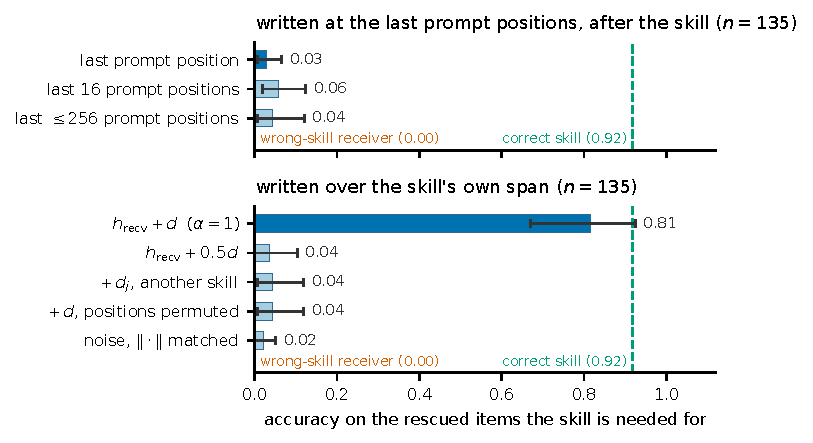
\includegraphics[width=\textwidth]{fig-channels-medcalc.pdf}
\caption{Matched position comparison on MedCalc with Qwen3-8B after the fix.
Both panels use layer $8$, the same wrong-skill receiver and $135$ items from
$14$ calculators. Left: donor states written at the last $1$, $16$, or up to
$256$ available positions after the skill. Right: interventions over the skill
span. The dashed line marks correct-skill accuracy; the dotted line marks
receiver accuracy. Error bars are calculator-bootstrap $95\%$ intervals.}
\label{fig:channels}
\end{figure*}

\paragraph{Dose, transfer, order and noise controls.}
Recovery changes nonlinearly with injection strength. On the screened subset
($n=135$, $14$ calculators), $\alpha=0.4,0.5,0.55$ gives
$0.04,0.04,0.14$ recovery, while $0.6,0.7,1.0$ gives $0.53,0.87,0.89$;
doubling the injection to $\alpha=2$ reduces recovery to $0.77$. Most of the
increase occurs between $0.55$ and $0.7$. To test content specificity, we
compare correct and other-skill injections over a common prefix length: the
correct prefix recovers $0.65$, whereas content from an unrelated skill
recovers $0.05$. A same-family mean control recovers $0.12$ on its $41$ eligible items.
Permuting positions also gives $0.05$, norm-matched Gaussian noise
gives $0.02$, and the identity control gives $0.00$. These controls show that
recovery depends on the injected content and its arrangement across positions,
rather than perturbation size alone.

\begin{table*}[tbp]
\caption{Span interventions on the screened MedCalc subset: $135$ items from
$14$ calculators, selected from $467$ rescued items across $48$ calculators
by requiring the wrong-skill receiver to solve no sampled item in a group.
The same-family control is available on $41$ items. Each row uses baselines
matched to its own items in Eq.~\ref{eq:rho}; accuracy intervals resample
calculators. Table~\ref{tab:replication} gives the interval for full-span recovery.}
\label{tab:big40}
\centering
\small
\begin{tabular}{@{}lrccc@{}}
\toprule
intervention & $n$ & accuracy & CI$_{95}$ & recovery $\rho$ \\
\midrule
\emph{correct skill in context} & $135$ & $0.919$ & $[0.844,\,0.976]$ & $+1.00$ \\
$h_{\text{recv}}+\dvec$ \ (full span) & $135$ & $0.815$ & $[0.670,\,0.925]$ & $+0.89$ \\
correct content, shared prefix & $135$ & $0.593$ & $[0.336,\,0.820]$ & $+0.65$ \\
half dose ($\alpha=0.5$) & $135$ & $0.037$ & $[0.000,\,0.103]$ & $+0.04$ \\
another skill (individual donor) & $135$ & $0.044$ & $[0.007,\,0.119]$ & $+0.05$ \\
mean from another skill family & $135$ & $0.044$ & $[0.012,\,0.102]$ & $+0.05$ \\
mean from the same skill family & $41$ & $0.122$ & $[0.000,\,0.250]$ & $+0.12$ \\
positions permuted & $135$ & $0.044$ & $[0.007,\,0.118]$ & $+0.05$ \\
norm-matched Gaussian noise & $135$ & $0.022$ & $[0.000,\,0.051]$ & $+0.02$ \\
\emph{identity intervention} & $135$ & $0.000$ & $[0.000,\,0.000]$ & $+0.00$ \\
\emph{wrong skill, unpatched} & $135$ & $0.000$ & $[0.000,\,0.000]$ & $+0.00$ \\
\bottomrule
\end{tabular}

\end{table*}

The receiver screen affects how these controls should be interpreted. On the
$34$ excluded calculators, the wrong-skill receiver already solves some items.
Other-skill content recovers $0.17$ on these groups ($n=332$), compared with
$0.05$ on the retained groups ($n=135$); noise recovers $0.10$ versus $0.02$.
This pattern is consistent with perturbations enabling knowledge already
available to the model, although it does not establish that mechanism.
A separate caveat is intervention size: skill spans in the screened subset
contain $365$--$1{,}630$ positions, far more than a single-position probe;
\S\ref{sec:posbudget} separates the number of written positions from their
arrangement.

\subsection{Which positions carry the effect}
\label{sec:posbudget}

Span injection writes $365$--$1{,}630$ positions; the final-position probe
writes one. To separate the arrangement of the span from the amount of state
it injects, we fix the number of written positions $B$ and vary only which
positions receive their own donor states, on the same $135$ items, layer and
receiver as Table~\ref{tab:big40} (Figure~\ref{fig:posbudget}).
\emph{Quantity does not explain recovery.} Evenly spaced or random subsets
recover at most $0.15$, even at half the span and half its content energy;
choosing the positions with the largest content change recovers at most
$0.12$; and writing states after the span stays at or below $0.07$, whether
the last $1$ to $234$ prompt positions at layer $8$ or the last $1$, the last
$16$ or all of them at each of seven layers from $4$ to $30$.
\emph{Contiguity does.} The same $256$ positions written as one block recover
$0.37$, and cutting that block into $2$, $4$, $8$, $16$ and $32$ evenly spaced
pieces lowers recovery to $0.24$, $0.22$, $0.13$, $0.08$ and $0.08$ at constant
budget and energy (one versus $32$ pieces: $+0.29$ [$0.09,0.48$], McNemar
$p<10^{-6}$). \emph{Location matters within the span.} A half-span block
centred on the procedure section recovers $0.82$ [$0.67,0.93$], close to the
full span; centred on the worked example it recovers $0.18$. \emph{Placement
must be exact.} Shifting every state by one position recovers $0.15$--$0.22$
with or without wrap-around, whereas leaving out the first or last $16$
positions and writing the rest in place keeps $0.89$--$0.92$. The skill's
effect is therefore carried by contiguous, correctly placed states of its
procedure-bearing tokens, not by the number of positions written or the
energy injected.

\begin{figure*}[tbp]
\centering
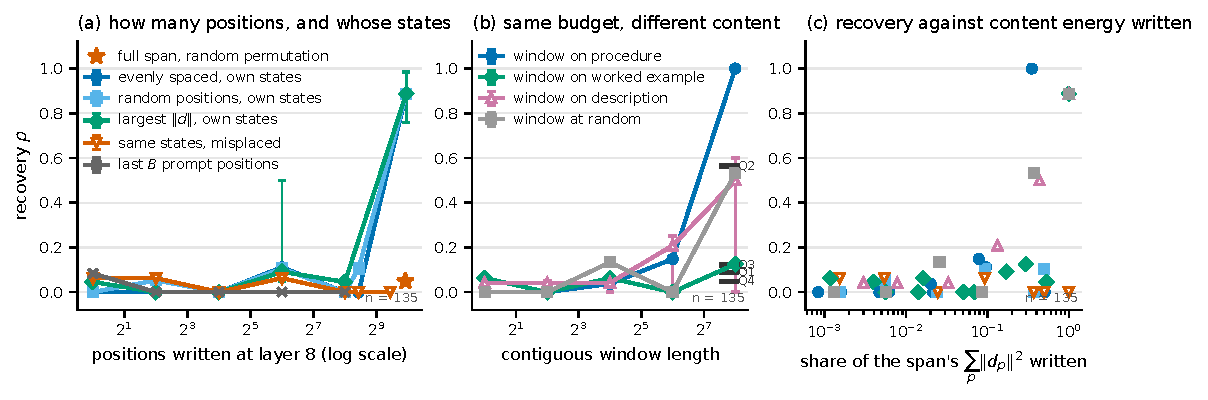
\includegraphics[width=0.72\textwidth]{fig-posbudget.pdf}
\caption{Position budget on MedCalc with Qwen3-8B, layer $8$: the same $135$
screened items ($14$ calculators) and wrong-skill receiver in every panel;
the dashed line is the whole span written in place ($\rho=0.89$). (a) $B$
positions, each written with its own donor state (evenly spaced, random, or
largest $\|d_p\|$), the same states written half a span away, or the last
$B$ prompt positions after the span. (b) A fixed budget written as $N$
contiguous blocks; dotted lines are random single positions at the same
budget. (c) One contiguous block centred on a section of the skill. (d) The
whole span displaced by $D$ positions, cyclically or without wrap-around;
triangles write it in place without its first or last $1$ or $16$
positions. Error bars are calculator-bootstrap $95\%$ intervals.}
\label{fig:posbudget}
\end{figure*}

\subsection{Skill identity and content within the span}
\label{sec:whose}

Table~\ref{tab:skillcontent} examines which content supports transfer and
whether it depends on the question. Of four contiguous span quarters, the
formula quarter gives the largest standalone recovery ($0.56$), compared with
$0.89$ for the full span. With the skill before the question, causal masking
prevents its states from depending on later question tokens: states are
identical across instances at equal prompt length and nearly identical
otherwise (cosine $\ge0.994$ over all $48$ calculators). Placing the skill after the question allows
such dependence. Even then, states from other instances of the same skill
recover $0.98$ at layer $8$, close to the current instance's $1.02$. At layer
$16$, the gap widens to $0.29$ versus $0.49$, while the instance-specific
remainder recovers little on its own. Early transfer therefore relies largely
on content shared across questions, with greater question dependence later.

\begin{table}[tbp]
\caption{Content and question dependence of span states, Qwen3-8B after the fix.
Top: each contiguous quarter is injected separately, on $135$ items from $14$
calculators. Bottom: with the skill after the question, content shared across
other instances and the instance-specific remainder are injected separately,
on $151$ items from $17$ calculators. Each comparison uses its screened subset
from the larger rerun. All entries report recovery $\rho$.}
\label{tab:skillcontent}
\centering\small
\begin{tabular}{@{}lcc@{}}
\toprule
\multicolumn{3}{@{}l}{\textit{Skill quarters, layer 8, skill before question} ($n=135$)} \\
Injected content & \multicolumn{2}{c}{Recovery $\rho$} \\
\midrule
Prose description & \multicolumn{2}{c}{$0.09$} \\
Formulas & \multicolumn{2}{c}{$0.56$} \\
Tool signatures & \multicolumn{2}{c}{$0.12$} \\
Worked example & \multicolumn{2}{c}{$0.05$} \\
Full span & \multicolumn{2}{c}{$0.89$} \\
\midrule
\multicolumn{3}{@{}l}{\textit{Question dependence, skill after question} ($n=151$)} \\
Injected content & Layer 8 & Layer 16 \\
\midrule
This instance & $1.02$ & $0.49$ \\
Other instances of the same skill & $0.98$ & $0.29$ \\
Instance-specific remainder & $0.03$ & $0.05$ \\
\bottomrule
\end{tabular}

\end{table}

Two completed corrected controls test whether a shared shift or a change in
state norm could explain recovery. Averaging content differences across skills
recovers only $0.03$ with the skill first ($n=135$) and $0.04$ with it last
($n=151$). Rescaling patched states to match the receiver's norm at each
position preserves $0.87$ recovery, compared with $0.89$ without rescaling.
In the corrected rerun, layer-$16$
recovery is $0.49$ with the skill last ($151$ items, $17$ calculators) and
$0.06$ with it first ($135$ items, $14$ calculators). Because these screens
retain different subsets, the contrast suggests sensitivity to prompt order
but is not a matched estimate of its effect (\extref{Appendix}{app:belongs}{extended version}).

\subsection{Rank required to recover the skill's effect}
\label{sec:rank}

We next inject the truncated matrix in Eq.~\ref{eq:rank} to measure how
recovery depends on the retained directions. Each intervention preserves the
same skill-specific mean at every span position, so the comparison tests how
much variation across positions is needed beyond that mean. At layer $8$ on
the screened MedCalc subset ($135$ items, $14$ calculators), recovery is
$0.07,0.05,0.12$ for $k=4,16,32$, rising to $0.63$ at $64$ and $0.77$ at
$128$, and reaching the untruncated $0.89$ at $256$ (Figure~\ref{fig:rank}).
Keeping the bottom $4$ to $128$ directions recovers at most $0.04$.
Recovery therefore depends on which directions are retained: the leading
directions support most of the measured effect, but a small number is
insufficient under this intervention.

For comparison across models, we summarise each curve by $k^{*}$: the first
rank reaching halfway from recovery at $k=16$ to the maximum on the fixed grid
$\{16,32,64,128\}$, with interpolation in $\log_2 k$. We call this the
\emph{rank knee}; it is not the minimum rank needed for full recovery.
Qwen3-8B gives $k^{*}=47$ [$43,55$], approximately $1.1\%$ of its hidden
width. \extref{Appendix}{app:rank2}{The extended version} reports development and deeper-layer curves.
These measurements describe what the injected representation can recover,
rather than directly measuring the model's unmodified computation: truncated
states may activate pathways absent from an unpatched run
\citep{makelov2024illusion}.

\begin{figure*}[tbp]
\centering
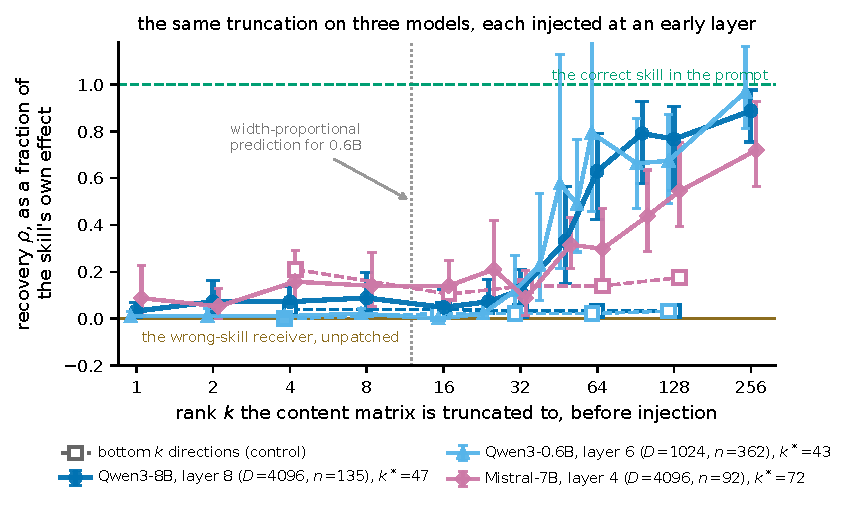
\includegraphics[width=0.88\textwidth]{fig-rank-medcalc.pdf}
\caption{Recovery after retaining $k$ leading centred directions and restoring
the positional mean, on MedCalc after the fix. Each model is injected at an
early layer. Despite a fourfold difference in hidden width, Qwen3-0.6B and
Qwen3-8B have similar rank knees ($43$ and $47$); Mistral-7B, with the same
width as Qwen3-8B, has $k^{*}=72$ [$46,94$]. Untruncated recovery is $0.89$,
$0.91$ and $0.84$, respectively, on each model's screened subset ($135$, $362$
and $92$ items). Both Qwen models reach that value by $k=256$ and Mistral-7B
at $k=384$. Dashed curves retain bottom directions. Error bars are
calculator-bootstrap $95\%$ intervals. Only complete rank experiments are
plotted.}
\label{fig:rank}
\end{figure*}

\subsection{Transfer depth and continued use of the skill}
\label{sec:where}
\label{sec:depth}

\paragraph{Span replacement and attention knockout separate in depth.}
Figure~\ref{fig:transferreading} compares transfer through span replacement
with continued use through attention on Qwen3-8B. Every layer is measured,
and both interventions are read on the same screened items. Replacement
recovers $0.92$--$0.98$ through layer $7$, $0.89$ at $8$ and $0.74$ at $12$
of $36$, then $0.16$ at $13$ and at most $0.07$ from $14$ onward ($n=135$,
$14$ calculators); the drop between layers $12$ and $13$ accounts for most of
the decline. We define the crossing below $\rho=0.5$ as the \emph{transfer
boundary} (labelled ``handover'' in the figures and tables). The
log-probability of the donor's generated reasoning also drops between these
layers, suggesting that binary answer grading sharpens, but does not fully
explain, the transition (Appendix~\ref{app:fullscale}). To test continued
reading, \emph{cumulative attention knockout} blocks attention to skill
tokens at every layer from $L$ onward. On the $134$ rescued items of the same
subset, $0.03$--$0.12$ stay correct for $L\le23$; this rises to $0.25$ at
$24$, first passes half at $25$ ($0.58$) and reaches $0.94$ at $35$. The
transfer boundary therefore lies at $13/36=0.36$ of depth and the reading
boundary at $25/36=0.69$, measured on the same items under the same screen.
Writing the last prompt position instead recovers at most $0.06$ at any
layer. Continued dependence on skill attention thus outlasts successful
transfer from the skill's states.

\begin{figure*}[tbp]
\centering
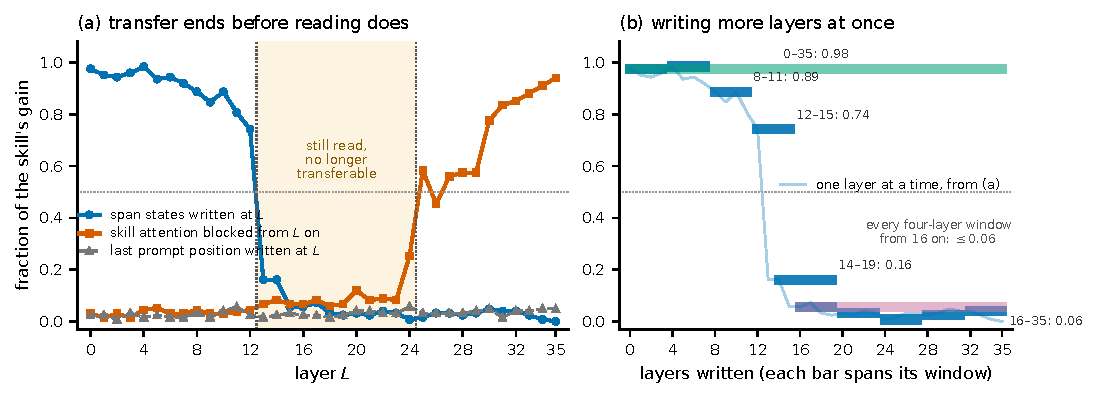
\includegraphics[width=0.96\textwidth]{fig-transfer-reading.pdf}
\caption{Transfer declines earlier than dependence on skill attention,
Qwen3-8B on MedCalc, with every layer measured. (a) Three interventions on
one axis and the same screened items ($n=135$; the knockout on their $134$
rescued items): span states written at layer $L$; attention to the skill
blocked from $L$ onward; and the last prompt position written at $L$. The
shaded band spans the layers where the skill is still read but no longer
transferable. (b) Each window is drawn across the layers it writes: four-layer
windows tile the stack, and the long windows $14$--$19$, $16$--$35$ and
$0$--$35$ are shown with them; the faint curve repeats (a). Writing every
layer at once recovers $0.98$, while any window starting at $16$ or later
stays at or below $0.06$. Span interventions use the corrected implementation;
attention knockout does not use state capture.}
\label{fig:transferreading}
\end{figure*}

\begin{table*}[tbp]
\caption{Replication with the corrected implementation. Injection layers are
$8$ for Qwen3-8B, $6$ for Qwen3-0.6B and $4$ for Mistral-7B. Recovery
intervals resample skill groups. Max control includes half-dose, other-skill,
permutation and noise comparisons, including same-family means available on
$41$ MedCalc/Qwen3-8B and $31$ MedCalc/Mistral items. $n$ describes the battery.
Handover brackets the transfer boundary as a fraction of model depth; reading
is the first layer, at one-layer resolution, from which blocking attention to
the skill still leaves at least half of the rescued items correct, measured on
the same screened items as the transfer boundary. $k^{*}$ is the rank knee on
the fixed grid.}
\label{tab:replication}
\centering
\footnotesize
\setlength{\tabcolsep}{4pt}
\begin{tabular}{@{}llrccccc@{}}
\toprule
task & model & $n$ (groups) & $\rho$ [95\% CI] & max control & handover & reading & $k^{*}$ \\
\midrule
MedCalc & Qwen3-8B & $135$ ($14$) & $0.89$ $[0.76,0.97]$ & $0.12$ & $0.33$--$0.36$ & $0.69$ & $47$ \\
TheoremQA & Qwen3-8B & $99$ ($75$) & $0.84$ $[0.75,0.92]$ & $0.25$ & $0.33$--$0.36$ & $0.58$ & $50$ \\
MedCalc & Qwen3-0.6B & $362$ ($38$) & $0.91$ $[0.75,1.05]$ & $0.30$ & $0.36$--$0.39$ & $0.79$ & $43$ \\
TheoremQA & Qwen3-0.6B & $132$ ($97$) & $0.74$ $[0.66,0.82]$ & $0.13$ & $0.36$--$0.39$ & $0.71$ & $52$ \\
MedCalc & Mistral-7B & $92$ ($20$) & $0.84$ $[0.69,1.09]$ & $0.35$ & $0.19$--$0.22$ & $0.84$ & $72$ \\
TheoremQA & Mistral-7B & $115$ ($94$) & $0.94$ $[0.84,1.05]$ & $0.27$ & $0.19$--$0.22$ & $0.59$ & $64$ \\
\bottomrule
\end{tabular}

\end{table*}

\paragraph{Adding late intervention layers does not restore transfer.}
To test whether a single late injection is simply too weak, we replace span
states repeatedly within consecutive layer windows, using the battery's
receiver and the same $135$ items as the depth sweep. Windows $8$--$11$,
$12$--$15$, $14$--$19$ and $16$--$35$ recover $0.89$, $0.74$, $0.16$ and
$0.06$; the last equals layer $16$ alone. Writing every layer at once
recovers $0.98$ [$0.91,1.03$], so the transplant itself remains effective when
it starts early enough; the identity control is exact on all $467$ items. On
TheoremQA ($99$ items, $75$ groups, with its battery's receiver), the same
windows recover $0.84,0.61,0.38,0.20$, the last again equal to layer $16$
alone. Repeated late injection therefore does not restore early-layer
recovery in these tests.

\paragraph{A spectral drop is not evidence of compression.}
Could the loss of transfer reflect compression into fewer dimensions? We
examine the centred participation ratio, a summary of how broadly matrix energy
is distributed across singular directions. It falls from $68$ at layer $12$
to $1.0$ at layer $16$, but this drop is driven by unusually large activations
\citep{sun2024massive, shi2026melayer}. In $35$ of $48$ calculators, one
token's state reaches $121$--$195$ times the median span norm, always on the
same two hidden dimensions. Removing the four highest-norm positions restores
the ratio to $85$ at layer $16$, and it stays between $62$ and $98$ over layers
$0$--$28$. The drop is also absent in Qwen3-0.6B and Qwen3-1.7B.
This diagnostic therefore does not support compression as the explanation
for lost transfer: a few large activations distort the dimensionality summary
(\extref{Appendix Table}{tab:prdiag}{extended version}).

\subsection{Replication across models and task domains}
\label{sec:ladder}

We extend span injection, rank truncation and the available depth comparisons
to Qwen3-0.6B ($D=1024$), Mistral-7B ($D=4096$, $32$ layers), and TheoremQA.
Each model is injected at an early layer, and the receiver screen is applied
separately to each run. Table~\ref{tab:replication} distinguishes completed
comparisons from missing controls or attention knockouts. Results for
Qwen3-1.7B, where skills rescue only $8$--$11\%$ of items, appear in \extref{Appendix Table}{tab:laddermodels}{the extended version}.

Span recovery ranges from $0.74$ to $0.94$ across the six model--task
combinations. The largest control is $0.35$, for a same-family
mean on $31$ Mistral/MedCalc items, where full-span recovery on the same items
is $0.71$. In every model--task combination, the transfer boundary occurs
before the reading boundary. The measured transfer boundaries lie at
$0.33$--$0.43$ of model depth within Qwen and at $0.19$--$0.22$ in Mistral.
Reading boundaries also vary by task: $0.58$--$0.71$ on TheoremQA and
$0.69$--$0.84$ on MedCalc across the three models.

The pre-registered width-proportional prediction places Qwen3-0.6B's rank
knee near $12$. Its observed recovery at $k=16,32,64,128$ is
$0.00,0.12,0.79,0.67$, giving $k^{*}=43$ [$39,52$], close to Qwen3-8B's
$47$ [$43,55$] despite the fourfold width difference. On TheoremQA, the
corresponding knees are $52$ [$46,62$] and $50$ [$39,67$], again inconsistent
with proportional scaling. Their participation ratios are also similar in
scale ($65$--$75$ versus $70$--$99$ over layers $0$--$20$, excluding unusually
large activations). Mistral, with the same width as Qwen3-8B, gives
$k^{*}=72$ [$46,94$] on MedCalc and $64$ [$50,79$] on TheoremQA: higher than
Qwen3-8B on both tasks, but with overlapping intervals. Its curve is also less
sharply defined, since recovery keeps rising past $k=128$ ($0.54$; $0.72$ at
$256$) and reaches its untruncated $0.84$ at $k=384$, against $256$ for
Qwen3-8B; its bottom-$k$ controls reach
$0.11$--$0.21$. The measured rank requirement is therefore not determined by
hidden width alone, while a difference between families is not established.

\paragraph{Readout checks.}
\label{sec:traps}
Alternative readouts can rank interventions differently. On the synthetic task,
averaged gold-answer log-probability favours a mean shared across skills by
$5.05$ nats despite lower accuracy ($0.251$ versus $0.288$, $358$ items).
Forcing an \texttt{ANSWER:} cue on MedCalc cuts the skill's accuracy gain from
$39.7$ to $4.7$ points ($0.178$ versus $0.131$ on $720$ items) while leaving a
$+1.08$ nat log-probability difference. Synthetic multiple
choice retains $0.54$ of the skill's effect after its numbers are corrupted and
$0.82$ after its lines are scrambled, illustrating possible answer-format
shortcuts
\citep{balepur2024artifacts} (\extref{Appendix}{app:traps}{extended version}). Other domains give limited evidence
(\extref{Appendix}{app:replication}{extended version}).


\section{Conclusion}

In the evaluated tasks and screened subsets, states across a skill's own
tokens transfer much of its effect, while a final-position intervention is more
sensitive to answer format---succeeding for compact answers, failing for
extended reasoning. Span recovery depends on content, position and multiple
leading directions. The rank knee does not scale proportionally with width
within Qwen, and a difference between model families is suggested but not
established. Across layers, states stop transferring most of the effect before
attention to them ceases to support performance, and the spectral drop does not
establish compression at that boundary. These findings distinguish what skill
states can transfer from how subsequent computation uses them.


\label{endmain}

\section*{AI Use Statement}
Generative AI tools assisted with manuscript restructuring and language editing,
literature lookup and reference checks, consistency checks between reported
results and local experiment records, and figure-label editing. The authors
are responsible for the final text, scientific claims and experimental artifacts.

\bibliographystyle{ACM-Reference-Format}
\bibliography{skillvector}

%% ================================================================= appendix
\appendix
%% Kept in both builds: what a reader needs to reproduce or scope the result.
% Appendix A -- setup, scope and experimental detail.
\section{Setup, in full}
\label{app:setup}

\paragraph{Two task families.} \emph{Real skills, the main material}:
MedCalc-Bench instances with the 55 gold calculator skills released with
SRA-Bench---$55$ calculators $\times$ $20$ instances $= 1{,}100$ items, graded
deterministically against a numeric tolerance with no model in the loop. Both
the skills and the tasks are other people's, which is what makes the effect size
credible. Qwen3-8B, single turn, no tools, greedy. Behavioural baseline and replication
intervals resample skill groups because items sharing a skill are dependent;
original item-level intervals in individual tables and plots are identified
separately in the main text.
\emph{A synthetic positive control}: a fictional unit system with a one-page
document giving its conversion table, so the no-document floor is guaranteed,
contamination is impossible, and we know exactly what content means. Items are
generated from the table ($n=358$), and every item whose answer appears in a
worked example is dropped.

\paragraph{Two dependent variables.} Accuracy, from a greedily decoded free-form
answer graded by the task's own scorer, and the teacher-forced log-probability of
the gold answer. They fail differently and disagree often enough that reporting
one alone is unsafe (\S\ref{sec:traps}); accuracy is read first throughout. No
item was rewritten into multiple choice to obtain an accuracy channel---%
\extref{\S}{sec:format}{The extended version} shows why that rewrite is not harmless.

\paragraph{How to read an arm's number.} Interventions are reported both as raw
accuracy and as the fraction of the range an intervention could possibly
recover,
\begin{equation}
\rho(\text{arm}) \;=\;
\frac{\text{acc}(\text{arm}) - \text{acc}(\text{receiver})}
     {\text{acc}(\text{donor}) - \text{acc}(\text{receiver})},
\end{equation}
where the receiver is the prompt being patched into, unpatched, and the donor is
the document actually in the prompt. $\rho$ is what transfers across settings and
raw accuracy is not: the four configurations in \extref{Figure}{fig:ladder}{the answer-length ladder} have
donors at $0.550$, $0.467$, $1.000$ and $0.950$ and receivers from $0.000$ to
$0.350$, and an earlier draft of this paper reported a channel as \emph{stronger}
under a longer answer by comparing $0.408$ against $1.000$ when as fractions
they are $0.87$ and $1.00$. Every figure axis labelled ``fraction'' is
Eq.~\ref{eq:rho}.

\paragraph{The instrument's own noise floor, measured.} Every decoding run
carries a \emph{null} arm: the receiver's own span states are captured and
written back over themselves. With a length-matched receiver this is a
bit-for-bit identity, so the null arm must equal the unpatched receiver at every
layer. Before the fix of Appendix~\ref{app:detail} it did not, quite. On
Qwen3-8B, across $1{,}766$ paired observations from every pre-fix run that
carries both arms, the null arm agrees with the receiver on $93.9\%$ of items:
$108$ flip, $46$ from wrong to right and $62$ from right to wrong, symmetric
within a sign test ($p = 0.15$). The pipeline itself is
deterministic---the same configuration run on two different machines agreed on
all $360$ item-by-arm cells---so this is not run-to-run variation but a
reproducible property of the instrument: the capture and decoding passes took
different attention kernels, which perturbs the written-back state by $1.2\%$ at
layer 8, and the dependent variable is the end of a chain of thought several
hundred tokens long, which is long enough for that to change an argmax somewhere
and propagate. It scales with the model: the same arm flips $0.6\%$ of items on
Qwen3-0.6B ($1{,}696$ pairs) and $0.8\%$ on Qwen3-1.7B ($1{,}338$), against
$6.1\%$ on the 8B. After the fix it is exact ($80/80$).

Three consequences are used throughout. First, \textbf{an effect smaller than
about six points is not resolvable on the 8B} in pre-fix runs, whatever a
binomial interval says. Second, the floor is not uniform: on the
persistent-failure cell it is $16\%$, between two and three times the average,
which is what one expects of items on a
decision boundary, so numbers read on that cell are read against a coarser
ruler. Third, on the restricted split the pre-fix null arm read $0.034$ rather than
zero---the split conditions on the receiver failing, so a flip there can only go
upward---so pre-fix span numbers are read against $0.034$; after the fix it reads
exactly $0.000$, the floor Table~\ref{tab:big40}'s $0.750$ is read against. We have rarely seen this control reported in the patching literature; at a single answer token it is small enough to be invisible, and it
becomes large only once the dependent variable is a long generation.

\paragraph{Four cells.}

Every item is labelled by what the document did to it: \textbf{R} (rescued:
wrong without, right with), \textbf{F} (persistent: wrong both ways), \textbf{K}
(kept: right both ways), \textbf{B} (broken: right without, wrong with).
\textbf{R is the only cell in which the document demonstrably works}, every table
here is read by cell, and \S\ref{sec:traps} shows the aggregate over all four can
be sign-inverted relative to R.



\subsection{Experimental detail}
\label{app:detail}

\paragraph{Models and numerics.} Qwen3-1.7B (28 layers, $d=2048$) and Qwen3-8B
(36 layers, $d=4096$); \S\ref{sec:ladder} adds Qwen3-0.6B (28 layers, $d=1024$)
and Mistral-7B-Instruct-v0.3 (32 layers, $d=4096$), whose chat template has no
system role, so the system text is merged into the user turn. Greedy decoding throughout, \texttt{enable\_thinking}
disabled and verified by a self-test on the rendered template. Eager attention
wherever an attention mask is manipulated, because sdpa and flash silently
ignore a 4D mask; layer-output hooks are implementation-independent, so the
decode-heavy runs use sdpa, which is about $2.5\times$ faster on a 2k-token
prompt. The 1.7B synthetic runs are fp32: bf16 costs $0.5$--$2.5$ nats on the
log-probability of a token deep in the tail, and every log-probability quantity
here is a difference of such numbers. The 8B runs are bf16 and the gaps we
report from them are $5$--$8$ nats, well outside that error; the accuracy
channel is immune to it either way.

\paragraph{Self-tests, and one that failed.} Three checks run with the
experiments. (i) \emph{Self-transplant}: donor and receiver are the same
forward, so the patch must be an exact no-op. On the fp32 synthetic runs the
deviation is $0.0$ nats at every layer. On the bf16 8B runs it is up to $0.38$
nats---bf16 arithmetic over two sequence lengths---while the accuracy channel
remains an exact no-op at every layer, which is how we tell the two apart.
(ii) \emph{Last-layer patch}: replacing the final layer's output at the patched
position makes that position's logits the donor's by construction, so the next
token must match exactly. (iii) \emph{Query-side control} for the knockouts.

\paragraph{An error worth recording.} The first version of the real-skill
scoring code patched at index $-1$ of a forward run over prompt \emph{and}
answer, which is the last token of the answer---after every position whose
logits are scored. Every arm returned the untouched baseline to six decimals,
which is what made it visible. Relative indices are the wrong default whenever
the forward length varies between the capture and the patch.

\paragraph{Control documents.} The synthetic controls are generated from the
skill document by \texttt{make\_controls.py}, which checks two things: the
corrupted document's numbers must not coincide with the task set's gold answers
(7 of 249 do, $2.8\%$), and the shuffle must not be the identity. All three
controls are stored under the same filename in separate directories, because the
injector derives the ``\# Skill: \emph{name}'' header from the file stem---a file
called \texttt{SKILL.\discretionary{}{}{}zorb-units.\discretionary{}{}{}corrupted.md} would announce the manipulation in
the prompt, and the control would then differ from the treatment in two ways.

\paragraph{Item set.} The synthetic set is generated from the conversion table
with the value range $2$--$40$, dropping any item whose answer also appears in a
worked example of the document ($n=358$; the sweeps use the first 120 or 200).
Distractors are values reachable by misreading the table---the neighbouring row,
the wrong family, the inverted direction---never random numbers, and the key is
rotated across A/B/C/D so a position-biased model still scores at chance.


\subsection{Evaluation scope and intervention provenance}
\label{app:limits}

\paragraph{An accidental replication.} A queueing mistake ran one $36$-layer
synthetic sweep ($358$ items, two arms, generations up to $900$ tokens) twice,
on two different GPUs in two different containers. All $36$ layer files agree
byte for byte. This does not bound the nondeterminism discussed in
\S\ref{sec:setup}---it is one configuration on one pair of devices---but it is
the only end-to-end check of it we have, and it came out exact.

\paragraph{Sample size and scope.} The battery was developed on $n=40$ (ten
calculators $\times$ four rescued instances), which gives intervals of roughly
$\pm 0.15$; \S\ref{sec:battery} reruns it on forty calculators and
\S\ref{sec:ladder} on further models and a second task, and the conclusions are
the ones that survived that. We report profiles and not individual layers: the one
non-monotonicity in the depth curve ($0.250$ at layer 18 against $0.475$ at 20)
has overlapping intervals and we do not interpret it. Among the three models,
Qwen3-1.7B is the weakest rung: the document rescues only $8$--$11\%$ of its
items, so its truncation curve is not resolved and is reported for completeness
rather than relied on. The width argument rests on Qwen3-0.6B against Qwen3-8B,
a factor of four within one family; a second family of the same width needs
more directions (\extref{Appendix}{app:replication}{extended version}).
In the pre-fix development runs, four independent shards recomputed the three baselines and agreed to the item
($0.950$ / $0.025$ / $0.175$), and the no-op arm sits on the receiver's baseline
at all twelve layers to within the $5\%$ numerical floor of
\S\ref{sec:cells}, so the instrument is checked even where the estimate is
coarse. The span channel, the depth sweep and the truncation curve have three
models and two tasks; the knockouts two models and two tasks; the final-position
results two models (Qwen3-1.7B, fp32); the document-order comparison and the
within-document localisation one.

\paragraph{Which items the causal claims are about.} Two restrictions stack.
Causal claims are made only on the rescued cell, the only cell in which the
document demonstrably works; on the persistent-failure cell the same arms track
the document rather than correctness---the transplant fails exactly where the
document fails---which is the right behaviour but is not a substitute for the
other cells. And within that cell the span arms are read on the calculators
whose \emph{receiver} never solves an item, because on the others the model does
not need the document, and before the fix any disruption of the wrong one,
noise included, let it fall back on what it already knows ($\rho = 0.14$ for
noise there against $0.00$ here). After the fix noise no longer does that
($0.00$ on those calculators), but a donor from another skill still reads $0.47$
there against $0.19$ on the rest. On forty calculators the restriction keeps fifteen of them and
$60$ items. On this split, accuracy is $0.750$ for the transplant and at most
$0.083$ for the tested negative controls; the main text distinguishes item-level
intervals from group-bootstrap uncertainty. Those forty calculators are
themselves the $160$ rescued items with the most instances per calculator, out
of $467$. We therefore reran the battery, the truncation curve, the depth sweep,
the dose curve and the within-document quarters over \emph{every} rescued item
of every calculator with at least two ($467$ items, $48$ calculators; the
restriction then keeps $135$ items over $14$). Every conclusion holds and no
control moves above $0.12$; Appendix~\ref{app:fullscale} gives the comparison
arm by arm.

\paragraph{What the rank result does and does not establish.}
\S\ref{sec:rank} truncates the injected content matrix to rank $k$ at a layer
where the untruncated version recovers most of the effect, and recovery stays near the control floor at $k \le 32$ while the bottom-$k$ control stays at the floor. That
licenses the forward direction: the effect requires directions of the same order
as the span's participation ratio, and within the Qwen family neither number
scales with width. It does not license a claim that the number belongs to the
document alone (Mistral-7B needs more), nor a converse about depth. Supplying a deep layer
with a higher-rank message taken from a shallow one does not restore the
handover ($\rho=0.00$ against $0.06$ for the same-layer donor, $0.00$ with the
norm matched), so we do not claim that what a deep layer lacks is rank.

\paragraph{Diagnostic results for the behavioural readout.} We could not find any
representational quantity at the final position that distinguishes the items a
skill rescues from the ones it does not: the norms and angles agree to three
digits, and the one similarity measure that separates them under the gold skill
separates them equally under a wrong one. And the document acts through a chain
of thought, so every causal measurement decodes several hundred tokens; scoring
under a forced \texttt{ANSWER:} cue instead leaves almost no behavioural effect
($0.178$ with the skill, $0.131$ without and $0.100$ with a wrong one, on $720$
items) while retaining a $+1.08$ nat log-probability difference---so the span
channel has no usable log-probability reading, and is reported on accuracy
alone.

\paragraph{An instrument fault, and which results predate its fix.} The state
capture called the model without an explicit attention mask while decoding
passed one; for a single unpadded sequence these are mathematically identical
but take different attention kernels, and they disagree by $1.2\%$ of the
state's magnitude at layer 8 and $25\%$ at layer 34. The visible consequence was
that the null arm---the receiver's own states written back over
themselves---changed the answer on $6.1\%$ of Qwen3-8B items. Passing the mask in
both makes the null arm exact ($80/80$ across two reruns) and leaves the transplant at
$\rho = 1.00$ as before. \emph{Rerun after the fix and reported from the
reruns}: Table~\ref{tab:big40} including the same-family donor, the
forty-calculator sufficiency curve, the layer windows, the forty-calculator rank
curve, the ten-calculator dose sweep and battery (Figure~\ref{fig:channels}),
the document-order comparison at layers $8$ and $16$, the within-document
quarters on ten and forty calculators, the Qwen3-0.6B truncation curve, and
every TheoremQA and Mistral-7B run; the attention knockout does not use the
capture path. \emph{Still from before the fix}: the synthetic tier and the
final-position sweeps, the ten-calculator development rank curve, the rank
curves at layers $12$ and $16$, the cross-layer donor, the Qwen3-0.6B depth
sweep and knockout on MedCalc, Qwen3-1.7B, the halves split, and
\extref{Figures}{fig:dose}{the dose and prompt-order figures}\ifextendedappendix\ and~\ref{fig:skilltask}\fi; these are read against a null
arm at $0.034$ rather than $0.000$ on the restricted split. Where a rerun
changed a conclusion---the worked example's share of the document, the
instance-specific part at layer $16$, the dose curve's shape---the text says
so.

\paragraph{Numerics.} Log-probabilities on the synthetic control are fp32,
because bf16 costs $0.5$--$2.5$ nats on a token deep in the tail. The 8B numbers
are bf16, which appears as self-transplant deviations of $0.1$--$1.1$ nats while
the accuracy channel remains an exact no-op; accuracy is read first throughout.




% Appendix -- the full-dataset rerun (kept in the WWW submission build).
\section{The full-dataset rerun, and what reads the span}
\label{app:fullscale}

Every MedCalc $\times$ Qwen3-8B result in the main text was developed on the
forty calculators with the most rescued items, sampling four each: $160$ of
$467$ rescued items, and $60$ items over $15$ calculators after the
receiver-never-solves restriction. We reran each of them with every rescued
item of every calculator that has at least two ($467$ items, $48$ calculators),
changing nothing else. The restriction is stricter on the larger set---a
calculator now has to fail on up to twenty items rather than four---so it keeps
$135$ items over $14$ calculators, and we also report the per-item restriction
($369$ items over $45$), which keeps the items whose own receiver fails.

\begin{table*}[tbp]
\caption{Full-dataset rerun against the subset the main text cites, Qwen3-8B on
MedCalc, layer $8$. Recovery is Eq.~\ref{eq:rho}; intervals are group bootstrap
over calculators. \emph{per-calc} is the main text's restriction, \emph{per-item}
the weaker one. Controls reach $0.12$ under the group screen and $0.25$ under
the item screen; each arm uses its own matched baselines.}
\label{tab:fullscale}
\centering
\small
\begin{tabular}{lccc}
\toprule
arm & full, per-calc ($n=135$) & subset ($n=60$) & full, per-item ($n=369$) \\
\midrule
transplant \texttt{real} & $\mathbf{0.89}$ $[0.76,0.97]$ & $0.87$ & $0.94$ \\
same skill, matched prefix & $0.65$ $[0.37,0.87]$ & $0.73$ & $0.84$ \\
\midrule
half dose $\alpha=0.5$ & $0.04$ & $0.06$ & $0.11$ \\
positions permuted & $0.05$ & $0.08$ & $0.21$ \\
norm-matched noise & $0.02$ & $0.10$ & $0.18$ \\
other calculator & $0.05$ & --- & $0.25$ \\
other family, mean & $0.05$ & $0.06$ & $0.16$ \\
same family, mean & $0.12$ $[0.00,0.25]$ & $0.05$ & $0.24$ \\
identity patch & $0.00$ $[0.00,0.00]$ & $0.00$ & $0.00$ \\
\midrule
rank $128$ / $64$ / $32$ / $16$ & $0.77/0.63/0.12/0.05$ & $0.77/0.54/0.13/0.06$ & $0.88/0.70/0.22/0.18$ \\
bottom-$64$ / bottom-$16$ & $0.03/0.04$ & $0.00/0.06$ & $0.11/0.12$ \\
quarters $q_0/q_1/q_2/q_3$ & $0.09/\mathbf{0.56}/0.12/0.05$ & $0.12/0.56/0.12/0.12$ & $0.18/0.64/0.22/0.19$ \\
\bottomrule
\end{tabular}
\end{table*}

The transplant, the truncation knee between $32$ and $64$ directions, and the
formula quarter's dominance all reproduce. The one arm that moves is the
same-family donor, from $0.05$ to $0.12$, on the $41$ items where it is defined.

\paragraph{The depth sweep at one-layer resolution.} The subset sweep measured
layers $0,4,8,12,14,15,16,20$ and placed the collapse somewhere after $12$.
At full scale we added $13$ and $17$--$19$:
recovery is $0.98,0.98,0.89,0.74$ at layers $0,4,8,12$, then
$0.16,0.16,0.06,0.06,0.07,0.03,0.02,0.03$ at $13$ through $20$ (per-calc; the
per-item restriction gives $1.00,0.98,0.94,0.79$ then
$0.32,0.34,0.25,0.25,0.23,0.19,0.14,0.17$). Layers $13$ and $14$ are
indistinguishable under both restrictions, so the transition is a single layer
between $12$ and $13$ and not the gradual decline a stride-$2$ sweep suggests.

\paragraph{A continuous dependent variable at the same boundary.} Accuracy over
a chain of thought is a threshold, and a smooth decline inside the model could
present as a step in it. We therefore decode the with-document trajectory once
per item and teacher-force that same trajectory under every other condition,
reading its mean token log-probability: $q = (\ell_L - \ell_{\text{recv}}) /
(\ell_{\text{gold}} - \ell_{\text{recv}})$ has the same two anchors as $\rho$
with no decoding threshold anywhere in it ($n=442$ items on which the document
run is correct, $48$ calculators). $q$ reads
$0.999, 0.989, 0.960, 0.831$ at layers $0,4,8,12$, then $0.598$
$[0.550,0.648]$ at $13$, $0.595$ at $14$, $0.340$ at $16$, $0.201$ at $20$ and
$0.129$ at $24$. Expressed per layer as a fraction of its range, the step at
$12\to13$ is $26.8\%$, against $3.7\%$ per layer over $8$--$12$ and $0.3\%$ from
$13$ to $14$: the discontinuity is present in a readout that cannot be produced
by grading. It is smaller than the behavioural step ($61\%$ of range), so the
grader sharpens the boundary roughly twofold without creating it, and it is
spread evenly across the four quarters of the trajectory ($0.20,0.26,0.31,0.21$)
rather than concentrated at the answer, which is the opposite of what a grading
artefact predicts. We also tried restricting $q$ to the tokens after the final
answer marker and report that it carries no information here: once the full
reasoning is teacher-forced, every condition predicts the final number almost
perfectly (median $\ell$ between $-0.001$ and $-0.005$ for all of them, and the
gold-minus-receiver denominator has median $0.0014$, below $0.01$ on $59\%$ of
items).

\paragraph{Which heads read the span.} For every attention head we recorded what
the span writes into the positions after it, as
$W_O^h \sum_{s \in \text{span}} a_{t,s} v_s$, and took its change between the
document and filler runs ($n=455$). Raw magnitudes are dominated by the last
layers, but the residual stream grows by more than an order of magnitude with
depth; normalised by it, the read-out concentrates in layers $12$--$21$ and
peaks at $18$. It is not a small circuit: of the $1{,}152$ heads the top $1\%$
carry $10.5\%$ of the read-out and the top $5\%$ carry $31.1\%$, and no head
attends to the span more than uniformly ($0.4$--$1.2\times$, with the span
occupying half the prompt). Blocking the $32$ highest-ranked heads' attention to
the span---ranked on half the calculators and evaluated on the held-out
half---costs $0.39$ of the document's effect, against $0.23$ for $32$ random
heads at the same layers (paired difference $0.154$, $95\%$ CI $[0.061,0.251]$,
McNemar $39$ versus $9$ discordant, $n=195$ over $23$ calculators). The ranking
is therefore causal, but it buys only $0.15$ over chance and $32$ heads remove
well under half the effect: the span is read diffusely, and we do not claim a
nameable set of reader heads. One further observation constrains what fails at
depth. After an injection at layer $L$, the span's own states from $L+1$ onward
are identical to the document run by construction---the span attends only to a
shared prefix and to itself---and the downstream per-head read-out of the span
is indeed $0.86$--$0.99$ of the document's at every injection layer we tried,
including those at which behaviour is gone. The content is present and is read;
what an injection at layer $16$ cannot undo is the reading that the question
positions already did at layers below it.


%% The technical report only. A WWW submission has 12 pages in total and the
%% main text takes 8 of them, so these do not fit; nothing here is deleted.
\ifextendedappendix
  % Appendix -- control documents and the three measurement traps.
\section{Control documents in full}
\label{app:controls}

$\dvec$ is defined by the document it is subtracted against, so ``content'' is
whatever separates the skill from that control. Our default control holds only
length fixed. Two tighter ones, generated from the skill document itself, hold
more: \textbf{shuffled} keeps every word and every number and destroys the line
order; \textbf{corrupted} keeps the wording, the procedure, the table layout and
the ordering of the units, and replaces \emph{every conversion factor}. All
three are injected under the same name and header, so the prompt never announces
which it is.

Both tighter controls move the accounting a long way
(Table~\ref{tab:controls}). A table whose numbers are all wrong solves $0.720$
of the rescued cell; a table with the right numbers in scrambled order solves
$0.659$; the unrelated text solves $0.098$. Against no document the cell is
$0.000$ by construction and with the gold document it is $1.000$. So when either
tight control is used, $\gvec$ is no longer inert---it repairs $0.63$--$0.74$---
and the residual $\dvec$ repairs only $0.17$--$0.28$.

\begin{table*}[tbp]
\caption{The same decomposition against three control documents. Synthetic
control, multiple choice, Qwen3-1.7B, $n=358$, rescued cell $n_R=82$, every
one of layers 21--27. ``in context'' is the control document actually placed in the prompt;
``$+\gvec$'' is its state injected at the final position of the no-document
prompt. That the two agree to within $0.03$ for three very different documents
is the strongest validity check we have on the patch itself. $\dvec$ is the
same measurement in all three rows; only what it is subtracted against changes.}
\label{tab:controls}
\centering
\small
\begin{tabular}{lccc}
\toprule
control document & \multicolumn{3}{c}{fraction of the rescued cell correct}\\
\cmidrule(lr){2-4}
 & control in context & $h_{\text{no}}+\gvec$ & $h_{\text{no}}+\dvec$ \\
\midrule
unrelated text, matched length      & 0.098 & \textbf{0.098} & \textbf{0.500--0.805} \\
same document, lines scrambled      & 0.659 & 0.634--0.671 & 0.171--0.280 \\
same document, factors replaced     & 0.720 & 0.720--0.744 & 0.171--0.256 \\
\midrule
gold skill in context & 1.000 & --- & --- \\
no document           & 0.000 & --- & --- \\
\bottomrule
\end{tabular}

\end{table*}

\paragraph{The same control on third-party skills.} We repeated the corrupted
control on the clinical calculators, where the arm already exists in the
released harness (numeric constants in the prose perturbed, wording, structure
and executable tools untouched). That material is free-form and answered through
a chain of thought, and there the corrupted skill is worth \emph{nothing}: on 20
rescued items it scores $0.050$, which is what no skill at all scores, against
$0.950$ for the gold skill. The synthetic and the real material therefore agree,
and they agree on the thing that matters---whether corrupting a document costs
you anything is a property of the answer format, not of the document.

Read as an attribution rather than as three competing estimates, this says
something uncomfortable about the multiple-choice form of the task. On the full
358 items the gold document is worth $0.179 \to 0.288$; a scrambled version of
it is worth $0.179 \to 0.268$ and a version with every factor wrong is worth
$0.179 \to 0.237$. Four fifths of the measured skill effect survives destroying
the order of the document, and just over half survives replacing every number
in it. What the model needs, in this format, is mostly a document containing the
right vocabulary and the right kinds of number---not a correct table. The
correct table is worth the remaining $0.02$--$0.05$ absolute, or $0.17$--$0.28$
of the rescued cell.

That is a statement about the answer format as much as about the model. We
registered the test before running it: in the free-form format the number has to
be produced, so a corrupted table should be worth nothing. It is
(Table~\ref{tab:format}). Corrupting every factor keeps $0.54$ of the
multiple-choice effect on the full item set and \emph{none} of the free-form
effect's $0.467$. Scrambling the line order costs little in either, which is what it
should: our shuffle permutes lines, and each row of the conversion table is one
line, so every factor is still there to be retrieved---just not in a readable
order.

\subsection{Multiple choice manufactures a floor and merges retrieval with
execution}
\label{sec:format}

Our synthetic items exist in two forms with identical content: four-option
multiple choice, and free-form (``give the number only''). The forms do not
measure the same thing, and there is a mechanism in the literature for why.
\citet{wiegreffe2025mcq} localise the choice of an answer \emph{symbol} to a
single middle layer and one to four attention heads per layer: in multiple
choice the decision is assembled into one position and one token. That is
exactly the regime in which a single-position patch transports the whole task,
and it is why our final-position channel reads $1.000$ there and $0.000$ under a
chain of thought on the same items.



Inspecting what the small model writes explains the top half. Without the
document it echoes the quantity from the question (``2''); with the document it
writes a \emph{conversion factor from the table} (``21'', ``180'', ``60''). It
retrieves and does not execute. Multiple choice scores retrieval as success
whenever the retrieved number can be matched against an option, and the
positional prior supplies a floor of $0.18$--$0.29$ on top.

The bottom half is the sharper version, and it is a prediction we registered
before running: if the multiple-choice form is solvable from a document's
structure rather than its numbers, a table with every factor replaced must score
near zero in free-form. It scores exactly zero.

Two consequences. A benchmark comparing skill effects across model scales in
multiple-choice format is measuring a mixture whose composition changes with
scale. And an ablation that perturbs a document and reports the accuracy drop is
measuring, in multiple choice, mostly whether the document is still recognisably
a document.

\section{Three measurement traps, in full}
\label{app:traps}

\subsection{The aggregate gold-answer log-probability ranks the controls first}

Averaged over all items, the log-probability of the gold answer under each
patched condition at layer 27, the last, orders as
\begin{center}
mean vector $-2.85$ \; $>$ \; filler state $-5.20$ \; $>$ \; \textbf{true skill
state} $-6.60$ \; $>$ \; no document $-7.30$ \; $>$ \; wrong skill $-10.29$,
\end{center}
i.e.\ a content-free average vector scores $3.75$ nats \emph{better} than the
state the model actually builds while reading the document, with accuracy
$0.256$ against that state's $0.436$.

The cells of \S\ref{sec:cells} account for the gap arithmetically
(Table~\ref{tab:cells}): F and B---where the document does not work---contribute
$133\%$ of it at layer 21, where the gap is $2.75$ nats, while on R the true state wins by $2.5$ nats and $0.69$ in
accuracy. The mechanism is visible in the option distribution: the mean vector
raises the entropy over the four answer tokens from $0.187$ to $0.972$ nats
(maximum $\ln 4 = 1.386$). A flattened distribution cannot assign any token
$-19$ nats, so it looks excellent exactly where the true state is confidently
wrong, and flattening never promotes a token to the argmax, so accuracy does not
move. The one point the two channels agree on is that the \emph{wrong skill} is
worst on both---positive evidence for content specificity, since injecting the
wrong content actively misleads.

The practical rule is that an aggregate log-probability over a mixed item set
measures confidence calibration as much as it measures content, and that a
decomposition by outcome cell is the cheapest way to tell which.

\subsection{A band where the forward pass is damaged}

Between layers 17 and 20 every patched condition improves together and the
conditions become indistinguishable. Reading by cell isolates the cause: on the
K cell---items the model already answers correctly---the true-state patch drops
the gold log-probability from $-1.6$ at layer 16 to $-7.1$ at layer 18, while
the filler-state patch, built over an equally long prompt, stays at $-1.5$. Any
transfer or recovery number falling in 17--20 is reported with that band marked.

\subsection{What the wrong-document control is actually worth}
\label{sec:plausible}


Holding the prompt's length, structure and the document slot's position fixed and
changing only what sits in that slot gives an ordered comparison the usual
binary---document or no document---cannot make. On the rescued items, with
everything else identical ($n=40$, intervals in brackets): no document at all
$0.025$ $[0.000, 0.073]$; non-clinical prose in the slot $0.250$
$[0.116, 0.384]$; this skill's own paired neutral document $0.175$
$[0.057, 0.293]$; one fixed wrong clinical skill $0.150$ $[0.039, 0.261]$; the
gold document $0.950$ $[0.882, 1.000]$.

Two things follow, one solid and one not. The solid one is that the
wrong-document control is not the same object as the no-document control: any
document in the slot moves these items off the floor, so a paper that reports
``with the document'' against ``without'' is measuring presence and content
together, and the presence part is not negligible on a cell selected for failing
without. That is the reason every arm in \S\ref{sec:battery} is measured against
a receiver that holds a document rather than against an empty slot.

The one that is not solid is the ordering. A clinical distractor costing more
than irrelevant prose ($0.150$ against $0.250$) is the direction we expected---a
near miss should be worse than an obvious miss, and the three conditions fall in
that order---but every pair of intervals overlaps at $n=40$, so we report a
direction and not a result. We flag it because the design that would settle it is cheap and
this material affords it: these 55 skills contain graded near misses by
construction (four different formulae for the corrected QT interval, two for the
delta gap), so ``how similar must a wrong document be before it hurts'' can be
measured on an ordered scale rather than a binary. We have not run that
experiment.




  % Appendix C -- the final prompt position.
\section{The geometry at the final position, in full}
\label{app:geometry}

Table~\ref{tab:behaviour} says the effect is content: a document that is present
but wrong is worth nothing. The internal picture at the last prompt position says
the opposite, and it says so exactly where the document is being read. The cosine
between the displacement caused by the skill and the displacement caused by an
unrelated document of similar length is $0.93$ at layer 0, $0.9475$ at layer 4
and $0.91$ at layer 10 on the synthetic control, falling to $0.35$--$0.41$ only
from layer 18, i.e.\ after the model has stopped reading (\S\ref{sec:where}). On
a second family the same comparison at layer 10 gives $0.9716$ between two
mutually exclusive skills against $0.9445$/$0.9555$ between each of them and an
unrelated document---a gap of $0.016$--$0.027$ with bootstrap intervals of width
$0.001$, so it is real and it is negligible.

Read alone, that says the injection is not content-specific. Under
Eq.~\ref{eq:decomp} it says something narrower and correct: over the first half
of the network $\|\dvec\|$ is only $0.38$--$0.45$ of $\|\tvec\|$, so most of what
a cosine between $h_{\text{skill}}$ and $h_{\text{wrong}}$ measures is shared,
and the interesting quantity is the part that is not. Three facts follow, all in
Figure~\ref{fig:decomp} with the numbers in Appendix~\ref{app:tables}. The
content component is a minority of the displacement wherever the document is
being read---under half of $\|\tvec\|$ through layer 14. Through layer 16
$\|\gvec\|$ actually exceeds $\|\tvec\|$: the \emph{wrong} document moves the
state further than the right one, and the two components partly cancel, which is
why the ratio recovers deeper without $\gvec$ shrinking. And two items' content
vectors are far more aligned when they use the same row of the conversion table
than when they do not, so whatever $\dvec$ encodes is about the document's
content rather than about the item.



None of this is causal evidence, and the rest of the paper is about why it
should not be read as any. A displacement can be large and do nothing; a
direction can differ systematically between documents and carry none of its
effect (\S\ref{sec:whose}). We use the geometry only to say which quantity is worth
intervening on, and then intervene.


\subsection{The decomposition and the answer-length ladder, in full}
\label{app:onepos}

We add each component back to the no-document state at the last prompt position
and let the forward pass continue, $h' = h_{\text{no}} + \alpha v$ for
$v \in \{\dvec_i, \gvec_i, \tvec_i, \bar{\dvec}, \dvec_j\}$, against an upper
reference that replaces the state outright with $h_{\text{skill}}$. The
protocol needs a task with an exact zero floor and a matched negative control,
so it is established on the synthetic tier and then carried to the clinical one;
Appendix~\ref{app:decomp} gives the full sweep, and this is the only place in
the paper where the synthetic material carries an argument of its own.

Three results, and the third is the one the rest of the paper uses.
\textbf{The presence component repairs nothing but is not inert}: injected
alone it takes the rescued cell to $0.098$, and putting the wrong document in
the prompt also gives $0.098$---it faithfully reproduces the behaviour of having
\emph{a} document, which is worse than having none. \textbf{The content
component repairs most of the cell}, $0.805$ against an upper reference of
$1.000$, having been dismissed by every geometric measurement as a small
residual. \textbf{The patch reproduces the document's whole behavioural
signature}: across the four cells, replacing the position with
$h_{\text{skill}}$ gives $1.000 / 0.000 / 1.000 / 0.000$ and adding $\dvec_i$
gives $0.805 / 0.075 / 1.000 / 0.186$---the same signature, attenuated. A patch
that only ever helped would be consistent with a generic ``try harder'' effect;
one that also breaks exactly the items the document breaks is carrying the
document's decision.

\paragraph{Which control you subtract chooses what you measure.} $\dvec$ is
defined against a control document, and the choice is a measurement decision
rather than a detail. Against an \emph{unrelated} document of the same length it
is topic, procedure and numbers together and repairs $0.805$ of the rescued
cell; against the \emph{same} document with every number replaced it is the
numbers alone and repairs $0.171$--$0.256$ (layers 21--27); against the same
document with its sentences shuffled, $0.171$--$0.280$. The three differ by a
factor of three to four, so a paper
that reports ``the content component'' without naming its control has not
specified the quantity. Appendix~\ref{app:controls} gives the full comparison.
\subsection{What a single position can carry is the answer, not the content}


Single-position patching is the standard move in this literature, and
Table~\ref{tab:causal} is a multiple-choice result, so it is worth asking what
that one position is carrying. The same items exist in a free-form numeric form,
where the answer is a number the model must compute rather than an option it
must select; there the skill is worth $0.006 \to 0.332$ and the rescued cell
has $119$ of the $358$ items.

Two things change and one does not. The ceiling collapses: through layer 22 no
condition exceeds $0.008$, including replacing the position outright with the
true skill state, and the best any single-position intervention achieves is
$0.235$, at layer 30. What does not change is the ordering---the content
component recovers $0.210$ and the presence component $0.008$---so the
conclusion of \S\ref{sec:decomp} survives the format while the magnitude does
not (full sweep in Appendix~\ref{app:tables}).

\paragraph{It is the format, not the model.} The identical sweep on the
\emph{same model and the same $358$ items} in multiple-choice form (Qwen3-8B,
$n_R=94$) recovers $0.957$ at layer 26 and $1.000$ at layers 29, 30 and 35.
Same model, same items, same intervention, same layers: $1.000$ when the answer
is one option letter, $0.235$ when it is a number the model has to produce.

The reason is mechanical and can be counted. The gold answers run one to five
tokens under this tokenizer and $341$ of the $358$ use two to four. A patch at
one prompt position can fix at most the first generated token; the rest are
produced in a context that still does not contain the conversion table.
Multiple choice compresses the answer to exactly one token---which is exactly
the unit a single-position patch transports. Patching the last $k$ positions
instead of one does \emph{not} lift the ceiling in proportion: $k=1,4,16$
recover $0.235$, $0.261$ and $0.403$, and $k=32,48,61$ recover $0.403$, $0.395$
and $0.370$, so sixteen positions carry about half of what the document carries,
four---the chat suffix---carry nothing extra, and everything past sixteen
carries nothing at all.

\paragraph{On third-party skills the same probe reads nothing.} There,
replacing the final prompt position with the with-skill state repairs at most 3
of 18 rescued items (layer 10) and 0--1 from layer 14 on and transplanting the question span---50 to 1697 positions, into a
length-matched receiver---repairs nothing beyond the receiver's own baseline at
any of seven layers (Table~\ref{tab:realspan}), with the self-transplant arm on
that baseline to the item, so the instrument is live and the null is real.
\S\ref{sec:battery} shows what does work on the same material.

\paragraph{Answer length is the cause, and that is a controlled comparison.}
The step from the synthetic tier to the clinical one changes the skill, the
task, the prompt length and the fraction of it a patch covers, so it cannot on
its own identify what makes the injection fail. We therefore made answer length
the only thing that moves: the \emph{same} 80 synthetic items, the same model,
the same document, prompted to reason step by step and give the answer on a
final \texttt{ANSWER:} line. In that format the skill is worth $0.000 \to
1.000$---every item is rescued, $F=K=B=0$---so there is more effect to recover
than in either other format, and the rescued cell is the whole item set.

The single-position patch recovers $\mathbf{0.000}$ of it
(\S\ref{sec:onepos}), as do $\dvec$ and $\gvec$. The last-layer
instrument check passes on 10 of 10 items in the same run.





\textbf{The range over which ``a skill's effect is carried by a vector'' is true
is the range over which the answer is short}---and the clinical result is then
not a property of that material but an instance of this.

\paragraph{It is a ceiling, and more positions do not raise it.} Patching one
position is a choice, not a measurement, so we repeated the sweep patching the
last $k$ prompt positions for $k \in \{1,4,16,32,48,61\}$, every one of the
$36$ layers. The no-document prompt is $61$--$63$ tokens, so $k=61$ writes all
of it and the ladder has no further rung. Recovery on the rescued cell, at each
$k$'s best layer, is $0.235$, $0.261$, $0.403$, $0.403$, $0.395$ and $0.370$,
and $0.403$ is also the largest value over every $k$ and every layer. Four
positions buy nothing---the last four tokens are the chat suffix---sixteen,
which reach back into the question, roughly double the recovery, and past
sixteen nothing is bought: at $k=32$ the items answered correctly are
item-for-item those answered correctly at $k=16$, with no discordant pair, and
at $k=61$ four are lost and none gained (exact McNemar $p=0.125$). We expected
the ladder to keep climbing and registered that prediction before the larger
$k$ ran; it does not climb.

The ceiling is therefore not a budget, and it is not an artefact of writing a
long prompt's states into a short one: the identical probe, receiver and donor
recover $1.000$ on the rescued cell of the multiple-choice format, where the
answer is one token at one position. What separates $0.403$ from $1.000$ is the
answer format.

It is \emph{not} explained by the patched positions being ones the document
does not occupy. On this same free-form material the document's own $688$
positions do no better: they recover $0.408$ at layer $0$, which is close to
putting the document back, and then at most $0.17$ from layer $3$ and nothing
from layer $15$ (Table~\ref{tab:windows2}), below what the last sixteen
positions reach. In free-form no channel on this task exceeds about $0.41$ at
any layer, so the ceiling is a property of the answer format rather than of
which positions are written. The comparison that does isolate position is on
the clinical material, where receiver, items and layer are held fixed: the
document's own span recovers $0.89$ and up to $256$ positions after it recover
$0.05$ (\S\ref{sec:decomp}).

One thing this ladder does not separate is the receiver. It patches into the
\emph{no-document} prompt, while span injection patches into a length-matched
\emph{wrong-document} one, so a receiver effect is not excluded here. Where we
have measured it---the same decomposition at the final position on the
synthetic multiple-choice task---the wrong-document receiver is never worse
than the no-document one and is better in the middle layers
(Table~\ref{tab:causal}), so it would move the ceiling the wrong way; but we
have not run it in free-form. We therefore read the low ceiling as a scope
condition on single-position and short-suffix patching under a multi-token
answer format, rather than as a negative result about $\dvec$. In a multiple-choice
item the answer \emph{is} one token at one position, so a patch that transports
the model's decision transports the whole task and looks like it transported the
document. What the final prompt position holds by layer 21 is the model's
\emph{answer}, not the document's content---consistent with the knockout result
that reading the document is finished by that layer (\S\ref{sec:where}).
\subsection{The decomposition on the synthetic tier, in full}
\label{app:decomp}

\paragraph{The geometry at that position says the opposite of the behaviour.}
Appendix~\ref{app:geometry} gives that measurement and why it cannot settle the
question on its own. We use geometry only to choose what to intervene on, and
then intervene.


We add each component back to the no-document state at the last prompt position
and let the forward pass continue: $h' = h_{\text{no}} + \alpha v$ for
$v \in \{\dvec_i, \gvec_i, \tvec_i, \bar{\dvec}, \dvec_j\}$. The upper reference
is replacing the state outright with $h_{\text{skill}}$; the lower reference is
no intervention.




Figure~\ref{fig:causal} is the causal counterpart of that geometry (numbers in
Table~\ref{tab:causal}, Appendix~\ref{app:tables}). Four of its curves are worth
reading separately.

\textbf{The presence component repairs nothing}---$0.098$, eight items of 82, at
every layer past 20, and $0.00$--$0.02$ before. It is not inert noise: injected
on its own it takes whole-set accuracy from the no-document baseline of $0.180$
to $0.151$, which is the accuracy of actually putting the wrong document in the
prompt. On the rescued cell it gives $0.098$, and the wrong document in context
also gives $0.098$. It faithfully reproduces the behaviour of having a document
present, and that behaviour is worse than having none.

\textbf{The content component repairs most of the cell}---$0.805$ at layer 26
against an upper reference of $1.000$, having been dismissed by every geometric
measurement in \S\ref{app:geometry} as a small residual.

\textbf{At one patched position it is under-scaled, not incomplete.} The
dose-response is monotone and steep---$\alpha=0.5,1,2$ give $0.31$, $0.81$,
$0.98$---so the missing $0.19$ at $\alpha=1$ is a magnitude deficit along a
correct direction, which is expected: $h_{\text{wrong}} + \dvec_i$ is exactly
$h_{\text{skill}}$, while adding $\dvec_i$ to $h_{\text{no}}$ lands elsewhere.
It does not generalise to more positions: at $k=16$ in free-form the dose is
flat between $\alpha=1$ and $2$ ($0.232$, $0.268$) and never approaches the full
replacement's $0.554$. The two components are additive by construction and not
additive in effect. What survives every configuration is the asymmetry: $\gvec$
alone is inert at every $k$, layer and $\alpha$.

\textbf{The receiver does not matter, and a single shared vector is not enough.}
Injecting $h_{\text{skill}}$ into the prompt that already holds the \emph{wrong}
document gives $0.979$--$1.000$, the same as into a prompt with no document---%
whatever the surrounding 700 tokens contribute, the final position does not need
it. But $\bar{\dvec}$, one vector for the whole item set, which is what ``a
reusable skill vector'' would mean, recovers $0.049$--$0.122$ from layer 21
against $0.500$--$0.805$ for the item's own. Splitting $\dvec_i$ along
$u=\bar{\dvec}/\|\bar{\dvec}\|$ and orthogonal to it and injecting each half
separates them and reverses the answer at layer 21: past it the parallel half
carries $\approx 0.9$ of the norm and $0.05$ of the effect while the orthogonal
half carries $0.44$ of the norm and $0.60$ of the $0.81$; before it the two swap,
inside the band \S\ref{sec:traps} independently identifies as one where the
forward pass is disturbed.

\paragraph{The patch reproduces the document's whole behavioural signature, not
just its successes.} Across all four cells, replacing the final position with
$h_{\text{skill}}$ gives $1.000 / 0.000 / 1.000 / 0.000$ on
rescued / persistent / kept / broken at layer 26 on the 1.7B, and
$1.000 / 0.024 / 1.000 / 0.000$ at layer 30 on the 8B---cell by cell, what the
document itself does by the definition of the cells. It reproduces the skill's
failures and its damage as faithfully as its repairs. Adding $\dvec_i$ gives
$0.805 / 0.075 / 1.000 / 0.186$ and $0.864 / 0.024 / 1.000 / 0.077$: the same
signature, attenuated. A patch that only ever helped would be consistent with a
generic ``try harder'' effect; one that also breaks exactly the items the
document breaks is carrying the document's decision. The presence component
passes the matching test against \emph{its} document: $h_{\text{no}}+\gvec$
scores $0.098$ on the rescued cell where the wrong document in context scores
$0.098$ (1.7B), and $0.250$ where it scores $0.250$ (8B), across four different
control documents (Appendix~\ref{app:controls}).




\begin{figure*}[tbp]
\centering
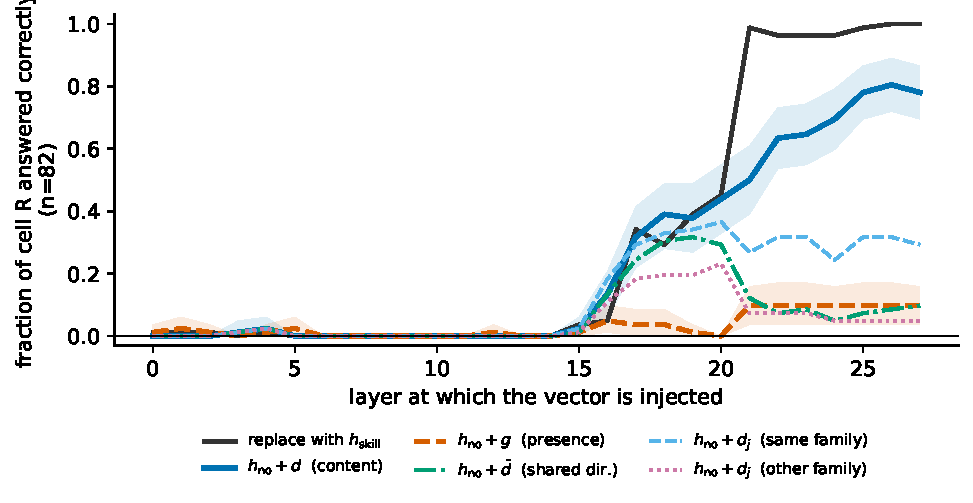
\includegraphics[width=0.86\textwidth]{fig-causal-tierA.pdf}
\caption{What each injected component repairs, on the cell the document
rescues. Shaded bands are bootstrap 95\% CIs for the two conditions the argument
rests on. $h_{\text{no}}+\tvec$ is omitted because it equals $h_{\text{skill}}$
identically and its curve lies under the black one---we run it, and it agrees
item by item. Synthetic control, multiple choice, Qwen3-1.7B, fp32, $n=358$,
rescued cell $n_R=82$.}
\label{fig:causal}
\end{figure*}

\begin{figure*}[tbp]
\centering
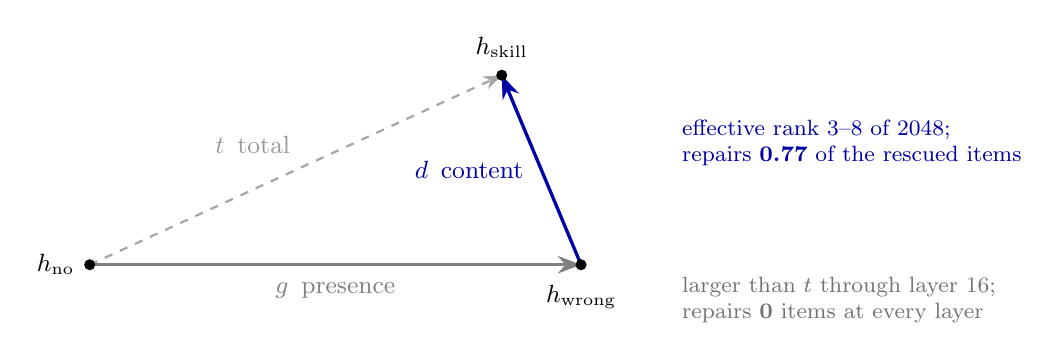
\begin{tikzpicture}[>=Stealth, every node/.style={font=\small}]
  \coordinate (no)  at (0,0);
  \coordinate (fil) at (6.24,0);
  \coordinate (yes) at (24.7:5.76);
  \draw[->, very thick, black!50] (no) -- (fil);
  \node[black!50, below=3pt] at ($ (no)!0.5!(fil) $) {$\gvec$\, presence};
  \draw[->, very thick, blue!65!black] (fil) -- (yes);
  \node[blue!65!black, left=3pt] at ($ (fil)!0.5!(yes) $) {$\dvec$\, content};
  \draw[->, thick, dashed, black!35] (no) -- (yes);
  \node[black!40, above left=-1pt and 6pt] at ($ (no)!0.55!(yes) $)
       {$\tvec$\, total};
  \fill (no) circle (2pt) node[left=2pt] {$h_{\text{no}}$};
  \fill (fil) circle (2pt) node[below=4pt] {$h_{\text{wrong}}$};
  \fill (yes) circle (2pt) node[above=3pt] {$h_{\text{skill}}$};
  \node[align=left, font=\footnotesize, black!55, anchor=west] at (7.4,-0.45)
    {larger than $\tvec$ through layer 16;\\
     repairs \textbf{0} items at every layer};
  \node[align=left, font=\footnotesize, blue!65!black, anchor=west] at (7.4,1.55)
    {effective rank 3--8 of 2048;\\
     repairs \textbf{0.77} of the rescued items};
\end{tikzpicture}
\caption{The decomposition, drawn to scale at layer 10 of the synthetic control
($\|\gvec\|=39.0$, $\|\dvec\|=16.3$, $\|\tvec\|=36.0$). A document of the right
length and the wrong content already moves the final prompt position most of the
way---in fact slightly further than the real skill does, which is why the
content arrow points partly back. Everything this paper is about is the short
blue arrow.}
\label{fig:schematic}
\end{figure*}

\begin{table*}[tbp]
\caption{The same items under two answer formats. Top: the effect itself. In
multiple choice the small model shows a $+11$pp skill effect over an $0.18$
floor; in free-form it shows nothing at all, over a floor of exactly zero, and
the effect appears only at 8B. Top block and the multiple-choice column of the
bottom block are the $358$-item reruns; the free-form control column is the
earlier $120$-item sample, which has not been rerun with the corrupted and
scrambled documents. Bottom: the same four documents under both formats, where
``share'' is $(\text{acc}-\text{none})/(\text{gold}-\text{none})$. Destroying
every number in the document keeps just over half of the effect in multiple
choice and none of it in free-form.}
\label{tab:format}
\centering
\small
\begin{tabular}{llcccc}
\toprule
model & format & no document & wrong document & gold skill & effect \\
\midrule
Qwen3-1.7B & multiple choice & 0.179 & 0.151 & 0.288 & $+10.9$pp \\
Qwen3-1.7B & free-form       & \textbf{0.000} & --- & \textbf{0.000} & $\mathbf{0}$ \\
Qwen3-8B   & multiple choice & 0.274 & 0.249 & 0.425 & $+15.1$pp \\
Qwen3-8B   & free-form       & \textbf{0.006} & \textbf{0.006} & \textbf{0.332} & $\mathbf{+32.6}$\textbf{pp} \\
\midrule
\multicolumn{2}{l}{document in context} & \multicolumn{2}{c}{multiple choice (1.7B)} & \multicolumn{2}{c}{free-form (8B)} \\
\multicolumn{2}{l}{} & acc & share & acc & share \\
\midrule
\multicolumn{2}{l}{none}                        & 0.179 & --- & 0.000 & --- \\
\multicolumn{2}{l}{same document, \emph{factors} replaced} & 0.237 & 0.54 & \textbf{0.000} & \textbf{0.00} \\
\multicolumn{2}{l}{same document, \emph{lines} scrambled}  & 0.268 & 0.82 & 0.325 & 0.70 \\
\multicolumn{2}{l}{gold skill}                  & 0.288 & 1.00 & 0.467 & 1.00 \\
\bottomrule
\end{tabular}
\end{table*}

\begin{figure*}[tbp]
\centering
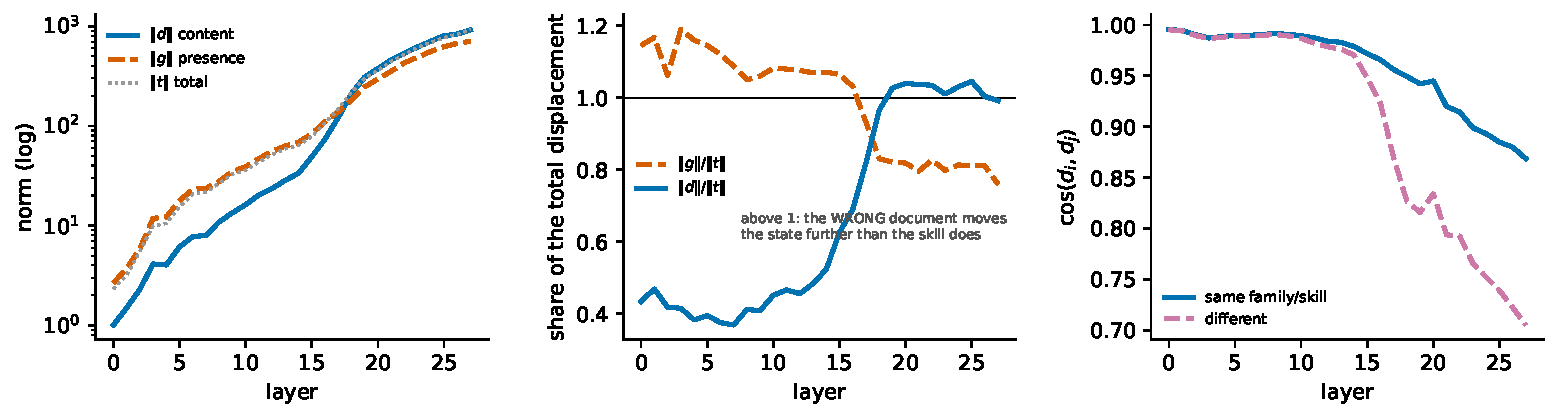
\includegraphics[width=\textwidth]{fig-decomp-tierA.pdf}
\caption{The decomposition across depth, synthetic control, Qwen3-1.7B, fp32,
$n=358$. Left: the three norms. Middle: each component as a share of the total
displacement; above $1$ the wrong document moves the state further than the skill
does, which is the case until layer 17. Right: how aligned two items' content
vectors are, split by whether they use the same row of the conversion table.}
\label{fig:decomp}
\end{figure*}

\begin{figure*}[tbp]
\centering
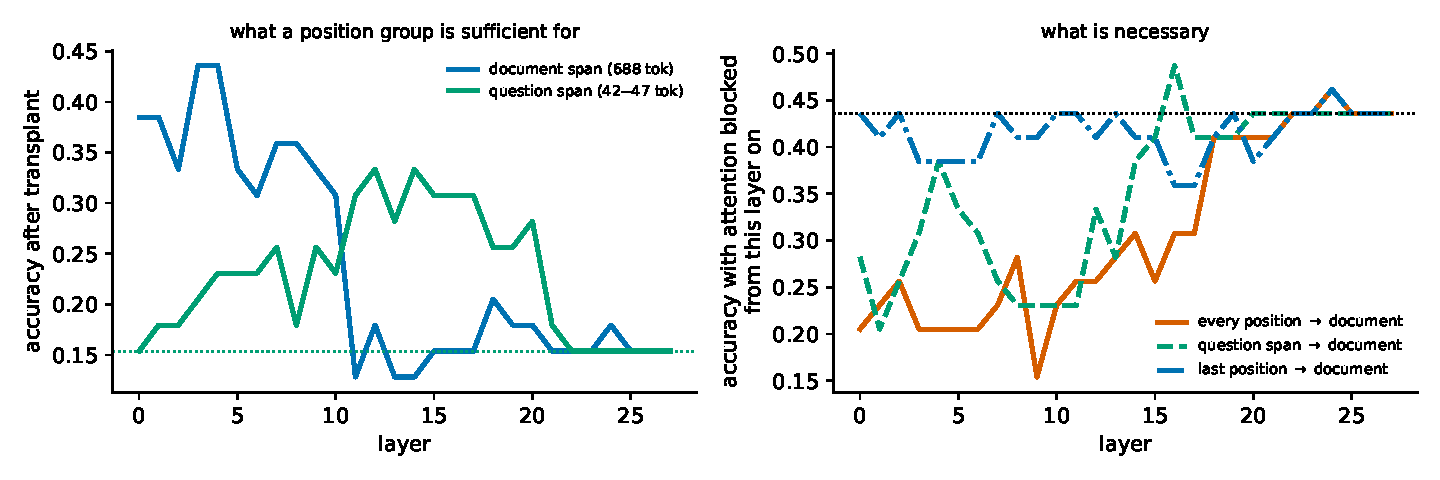
\includegraphics[width=\textwidth]{fig-windows-tierA.pdf}
\caption{Left: what each position group is sufficient for, as a function of the
layer at which its states are transplanted; dotted lines are each channel's own
receiver baseline. Right: what is necessary---accuracy when attention to the
document is masked from the given layer to the end, cumulatively; the dotted
line is the unmasked baseline. Synthetic control, multiple choice, Qwen3-1.7B,
$n=39$.}
\label{fig:windows}
\end{figure*}

\begin{table*}[tbp]
\caption{Peak accuracy of each transplant channel, by model and answer format.
``Donor'' is the with-skill forward and ``receiver'' the prompt being patched
into; the two span channels patch into a length-matched filler-substituted
prompt, the final-position channel into the no-document prompt, which is why
their baselines differ. The final-position rows are the $358$-item reruns; the
two span channels are the earlier $39$-item transplant runs, which were not
rerun. Peaks in \textbf{bold} where the channel recovers most
of the donor.}
\label{tab:windows2}
\centering
\small
\begin{tabular}{llccc}
\toprule
channel & configuration & recv. & peak (layers) & donor \\
\midrule
\multirow{3}{*}{document span (688 tok)}
 & 1.7B, multiple choice & 0.154 & \textbf{0.436} (3--4) & 0.436 \\
 & 8B, multiple choice   & 0.233 & \textbf{0.575} (0--6) & 0.550 \\
 & 8B, free-form         & 0.008 & 0.408 (0 only)        & 0.467 \\
\midrule
\multirow{3}{*}{question span (26--50 tok)\hspace{-2mm}}
 & 1.7B, multiple choice & 0.154 & 0.333 (12--14)        & 0.436 \\
 & 8B, multiple choice   & 0.233 & \textbf{0.517} (21)   & 0.550 \\
 & 8B, free-form         & 0.008 & 0.025 (any, i.e.\ none) & 0.467 \\
\midrule
\multirow{3}{*}{final position(s)}
 & 1.7B, MC, rescued cell & 0.000 & \textbf{1.000} (26--27) & 1.000 \\
 & 8B, MC, rescued cell   & 0.000 & \textbf{1.000} (29--35) & 1.000 \\
 & 8B, free-form, rescued cell & 0.000 & 0.235 ($k$=1), 0.403 ($k$=16) & 1.000 \\
\bottomrule
\end{tabular}
\end{table*}

\begin{table*}[tbp]
\caption{Question-span transplants on the same material and construction.
\emph{Which} positions are transplanted is the whole difference between this
table and Table~\ref{tab:realspandepth}.}
\label{tab:realspan}
\centering
\small
\begin{tabular}{lccccc}
\toprule
transplanted positions & donor & L0--12 & L16 & L22 & L30 \\
\midrule
\multirow{2}{*}{question span (50--1697 pos., $n=40$)}
 & the gold skill   & 0.10--0.23 & 0.150 & 0.200 & 0.154 \\
 & the receiver itself (no-op) & 0.13--0.20 & 0.175 & 0.125 & 0.154 \\
\midrule
\multicolumn{2}{l}{no document / the gold skill in context}
 & \multicolumn{4}{c}{0.025 \quad / \quad 0.950} \\
\bottomrule
\end{tabular}
\end{table*}


  % Appendix D -- the skill span.
\section{The span battery, in full}
\label{app:battery}

\S\ref{sec:onepos} is a negative result about a probe, not about a model. The
probe fails because one position cannot hold a decision that occupies hundreds
of tokens. The obvious repair is to stop using one position, and the natural
place to use instead is the one group of positions whose size grows with the
document: the document's own tokens.

\paragraph{The receiver.} The donor is the with-document forward; the receiver
is the \emph{same prompt} with the document's tokens overwritten, one for one,
by the tokens of \emph{one fixed clinical skill document}---the same document
for every instance and every skill, and the gold document of none of them.

Both halves of that choice were forced by measurement. It has to be fixed,
because a receiver built from each skill's own paired control makes the
receiver's states depend on the instance, and then every arm of the form
$h_{\text{recv}} + (\cdot)$ inherits an instance-dependent floor; measured, the
with-document states vary across a skill's instances by a relative
$3.5\times10^{-3}$ while such a receiver's vary by $0.36$. We use a
\emph{clinical} document rather than neutral prose because it is the same
condition the behavioural runs call
``wrong skill'', so the receiver's baseline means what the paper's presence
effect means; \S\ref{sec:plausible} measures the two side by side and finds them
close ($0.150$ against $0.250$, $n=40$, overlapping intervals).

Length-matching is not a refinement here either, it is the whole experiment. An
earlier version of this run used the no-document
prompt, which is some $900$ tokens shorter, and aligned the spans by their ends;
the real arm and the wrong-document arm then both read $0.200$---the signature
of two arms broken in the same way by a rotary phase shift, which is easy to
read as an absent effect. With a matched receiver every position keeps its
index, the two sequences are identical outside the span, and the question span
is verified token-identical between donor and receiver before anything is
patched.

Because the receiver already holds a document, the substitution obeys
$h_{\text{recv}}(\text{span}) + \dvec(\text{span}) = h_{\text{skill}}(\text{span})$: it is $h_{\text{recv}} + \dvec$ at $\alpha=1$. That is
what makes the rest of this section possible.

\paragraph{It carries, completely.} Figure~\ref{fig:channels} puts the two
channels side by side on the same model and the same decomposition. At the last
prompt position, five arms---including replacing the entire state with the
with-document one---sit between $0.050$ and $0.150$ against a no-document
baseline of $0.050$. Over the document's own span, after the instrument fix,
the corresponding span content matrix gives $1.00$ against a receiver at $0.00$ ($n=16$, four
calculators).

Before the fix the same panel read $0.950$ on twenty items, $\rho = 1.06$: the
transplant and the document disagreed on one item and the transplant got it
right. The honest reading of every $\rho$ near or above $1$ here is
``indistinguishable from having the document in the prompt''.



\paragraph{How deep the handover works (before the fix).} Transplanting the \emph{document's own}
states over the same construction recovers the document's entire effect through
layer 12 and then falls off a cliff (Table~\ref{tab:realspandepth}). Layer 0 is
close to tautological---a layer's output over the document's tokens is not far
from putting those tokens back---so the load-bearing entries are layers 8 and
12, a third of the way into
the network, where the receiver has already processed eight or twelve blocks'
worth of filler in those positions and the transplant still recovers
everything. Past layer 14 a single layer's worth stops being enough: $\rho =
0.14$ at 15 and 16, and $0.00$ at 24 and 30. Writing
the span at \emph{every} layer at once returns it to $\rho = 1.00$, so what
fails past layer 14 is the handover at one depth, not the mechanism.

\paragraph{The profile replicates; its one anomaly does not.} We ran the sweep a
second time on the same items against the other receiver---the single fixed
wrong skill rather than each skill's paired control---and the two agree wherever
the first is well behaved: $+1.00$ against $+1.00$ at layer 0, $+1.06$ against
$+1.07$ at 4, $+1.03$ against $+1.14$ at 8, $+0.81$ against $+1.00$ at 12
(Table~\ref{tab:realspanfixed}). The single bump in the first run, $\rho=0.07$
at layer 18 against $0.29$ at 20, does not survive: the replication gives $+0.16$
at layer 20, below its own layer 16. We read the profile and not the individual
layers, and we read that bump as noise.



The surviving window is a window in \emph{relative} depth: layers 0--12 of 36
here, 0--10 of 28 on the synthetic tier, both about a third of the way in.



\paragraph{It behaves like a mechanism, not like a perturbation.} Four
controls, all at layer $8$, all in Figure~\ref{fig:channels}, and all read on
the calculators a wrong document never rescues.

\emph{Dose}: after the fix, $\alpha = 0.4, 0.5, 0.55, 0.6, 0.7, 1, 2$ give
$\rho = 0.06, 0.00, 0.06, 0.62, 0.94, 1.00, 0.81$ ($n=16$). The transition is a
step and not a ramp---half the content is no better than none of it, since the
state is then a midpoint between two coherent documents and corresponds to
neither---and overshooting costs a little. An injection that merely had to be
large would show neither. Before the fix the same sweep read $0.17, 0.03, 0.17,
0.88, 0.97, 1.00$ ($n=30$), and a coarser one $0.06, 1.06, 1.06, 0.89$ at
$\alpha = 0.5, 0.75, 1, 2$ with the per-position rescaled doses coinciding
($0.06$ and $0.89$ both ways).

\emph{Transfer}: after the fix, another skill's vector over the prefix the two
documents share gives $0.19$ against $0.94$ for this skill's own vector on the
same positions ($n=16$), and on forty calculators a donor from another family
$0.06$ and one from the same family $0.06$ against $0.73$. Before the fix, the
mean content vector of a \emph{different} skill, written over the prefix the two
documents share, gave $\rho = 0.06$ against $1.00$ for
this document's own vector written over \emph{the same positions}. Because every
skill's vector is taken against the same fixed control, this arm is exactly that
skill's own span states rather than a hybrid, so it is the cleanest form the
transfer test can take; and the paired control is what makes it a statement about
content rather than about how many positions were patched.

\emph{Order}: the same vectors, permuted across the span's own positions, give
$\rho = 0.00$ ($n=16$) and $0.08$ on forty calculators after the fix ($0.12$
before). The span is not a bag---which position holds which part of the
document is most of the effect.

\emph{Norm}: Gaussian noise rescaled to each position's $\|\dvec\|$ gives
$\rho = 0.00$, exactly the receiver ($0.10$ on forty calculators). The effect is not a consequence of writing
something large into those positions.

\paragraph{The split these four are read on, and why it is not cherry-picking.}
On four of the ten calculators the receiver---a wrong clinical document---already
solves the items. Before the fix every span arm worked there: a related-skill
donor scored $\rho = 0.71$, an unrelated one $0.43$ and norm-matched
\emph{noise} $0.14$, against $0.00$, $0.06$ and $0.00$ on the five where the
receiver scores zero, and pooling the two groups turned a null transfer arm into
an apparent $\rho = 0.38$. After the fix six calculators fall on that side;
noise no longer works there ($0.00$, $n=24$) but another skill's vector still
reads $0.47$ against $0.19$ on the four restricted calculators: there the wrong
document in the slot was leading the model astray, and a coherent replacement
lets it fall back on a formula it already knows.

The split conditions on the \emph{receiver}, which is a control, and on no
intervention arm, so it cannot manufacture the contrast it is used to report; and
it is taken per calculator rather than per instance because ``this model can do
this calculator unaided'' is a property of the calculator. Table~\ref{tab:battery-all}
gives every arm on all forty items for comparison.

\paragraph{It replicates on four times as many skills.} The ten calculators
above are the ten with the most rescued instances, and twenty items from five
calculators is the single most obvious reason to stop reading. We therefore ran
the battery on \emph{forty} calculators, recomputing the restriction inside the
larger set rather than carrying it over. Of the forty, fifteen are calculators
the wrong document never rescues, which leaves $60$ items---three times the
original---and every arm holds (Table~\ref{tab:big40}): the document's own
vector recovers $\rho = 0.87$, the same vector over only the prefix another skill's document shares $0.73$, half a dose
$0.06$, a donor from another family $0.06$, permutation of the span's own
positions $0.08$, and norm-matched noise $0.10$, against a null arm at exactly
$0.00$ and a receiver at exactly $0.000$, and a donor from the same family
$0.06$ (rerun after the instrument fix). The separation is
between $0.87$ and at most $0.10$, on three times the material, with
item-level intervals as identified in the main-text caption.



\paragraph{And it fails where the document fails (before the fix).} On the
persistent-failure cell---items the gold document does \emph{not} rescue---the
same transplant at the same layer gives $0.100$, equal to the receiver's $0.100$,
against the document's own $0.025$ ($n=40$, ten calculators; the null arm read
$0.150$ in this run). The channel transports what the document does, including doing
nothing. An arm that only ever helped would be consistent with a generic ``try
harder'' effect; this one is not.

\paragraph{Why it can carry when a single position cannot.} The span is $415$ to
$1{,}630$ positions wide on the forty calculators, the same order as the answer it has to support. This is the
positive half of \S\ref{sec:onepos}'s capacity statement, and the two together
give the rule the paper is built on: \emph{a patch transports what fits in the
positions it is given}. A one-token answer fits at one position; a chain of
thought fits nowhere except on a group of positions as large as the document
itself.


\begin{table}[tbp]
\caption{Behaviour on the real skills, Qwen3-8B, all three arms on the same
$1{,}100$ items, CIs bootstrapped over the 55 calculators. The presence effect
(wrong skill minus no skill) is a clean zero, so the $+39.7$pp is content.}
\label{tab:behaviour}
\centering
\small
\begin{tabular}{lrcc}
\toprule
& $n$ & accuracy & 95\% CI \\
\midrule
gold skill                & 1100 & 74.2\% & [65.8, 81.8] \\
no skill                  & 1100 & 34.5\% & [26.5, 42.8] \\
wrong skill (length-matched) & 1100 & 31.5\% & [23.7, 39.5] \\
\midrule
gold $-$ no skill         & 1100 & $+39.7$pp & [$+31.7$, $+47.7$] \\
gold $-$ wrong skill      & 1100 & $+42.6$pp & [$+34.7$, $+50.5$] \\
\textbf{presence: wrong $-$ no skill} & 1100 & $\mathbf{-2.9}$\textbf{pp} & [$-8.8$, $+3.0$] \\
\bottomrule
\end{tabular}
\end{table}

\begin{table*}[tbp]
\caption{The document-span transplant by layer. Qwen3-8B, 55 third-party
clinical skills, the $40$ rescued items, the full chain of thought decoded and
graded by the task's own scorer. The receiver is the with-skill prompt with the
document's tokens replaced by a filler document, before the instrument fix, so it is the same length and
every transplanted position keeps its rotary phase. Restricted, as everywhere in
this section, to the calculators the receiver never solves. This sweep used each
skill's paired control as the filler and the battery of \S\ref{sec:battery} the
single fixed one; over all forty items the three baselines agree to within
$0.01$ across the two ($0.175$/$0.025$/$0.950$ against $0.167$/$0.028$/$0.944$),
so the profile does not depend on that choice---the unrestricted version is
Table~\ref{tab:realspan-all}. The no-op arm---the receiver's own states written
back into the receiver---is reported wherever it was run and must equal the
receiver's baseline; it does, at every layer.}
\label{tab:realspandepth}
\centering
\small
\begin{tabular}{@{}rccc@{}}
\toprule
layer & accuracy & CI$_{95}$ & fraction of the document's own effect \\
\midrule
0 & $0.875$ & $[0.713,\,1.000]$ & $+1.00$ \quad\tiny(no-op arm 0.000) \\
4 & $0.938$ & $[0.819,\,1.000]$ & $+1.07$ \\
8 & $1.000$ & $[1.000,\,1.000]$ & $+1.14$ \\
12 & $0.875$ & $[0.713,\,1.000]$ & $+1.00$ \quad\tiny(no-op arm 0.000) \\
13 & $0.625$ & $[0.388,\,0.862]$ & $+0.71$ \quad\tiny(no-op arm 0.000) \\
14 & $0.688$ & $[0.460,\,0.915]$ & $+0.79$ \quad\tiny(no-op arm 0.000) \\
15 & $0.125$ & $[0.000,\,0.287]$ & $+0.14$ \quad\tiny(no-op arm 0.000) \\
16 & $0.125$ & $[0.000,\,0.287]$ & $+0.14$ \quad\tiny(no-op arm 0.000) \\
18 & $0.062$ & $[0.000,\,0.181]$ & $+0.07$ \quad\tiny(no-op arm 0.000) \\
20 & $0.250$ & $[0.038,\,0.462]$ & $+0.29$ \\
24 & $0.000$ & $[0.000,\,0.000]$ & $+0.00$ \\
30 & $0.000$ & $[0.000,\,0.000]$ & $+0.00$ \quad\tiny(no-op arm 0.000) \\
\midrule
every layer & $0.875$ & $[0.713,\,1.000]$ & $+1.00$ \\
\midrule
\emph{the filler document, unpatched} & $0.000$ & & $0.00$ \\
\emph{the gold document in context} & $0.875$ & & $1.00$ \\
\bottomrule
\end{tabular}

\end{table*}

\begin{table*}[tbp]
\caption{Geometry of the content component over the document's own span, by
layer, Qwen3-8B, $n=40$, all against the same fixed control document. Unlike the
same quantity at the final prompt position, this vector is the size of the state
it displaces. Two skills' vectors are substantially aligned and most of each
one's energy lies along the all-skill mean---which, injected alone, recovers
$0.11$ here and $0.06$ with the document after the question (both pre-fix)
(\S\ref{sec:whose:docklast}). Participation ratios are centred, so they
count the directions the span's positions \emph{differ} in. Cosines between
content vectors depend on which control was subtracted: against each skill's own
paired control the cross-skill cosine reads $0.10$ instead of $0.54$, which is a
fact about the control and not about the skills.}
\label{tab:geometry}
\centering
\small
\begin{tabular}{@{}rccccccc@{}}
\toprule
layer & $\|\dvec\|$ & $\cos(\dvec_i,\bar{\dvec})$ & energy along $\bar{\dvec}$ & $\|\dvec\|/\|h\|$ & PR$(\dvec)$ & PR$(h_{\text{skill}})$ & $\cos(\dvec_i,\dvec_k)$, other skill \\
\midrule
0 & $10$ & $0.720$ & $0.54$ & $0.91$ & $81.8$ & $50.5$ & $0.483$ \\
4 & $28$ & $0.738$ & $0.56$ & $0.94$ & $77.1$ & $45.7$ & $0.511$ \\
8 & $53$ & $0.755$ & $0.58$ & $1.04$ & $94.8$ & $63.8$ & $0.539$ \\
12 & $68$ & $0.766$ & $0.60$ & $1.09$ & $64.2$ & $46.3$ & $0.560$ \\
16 & $106$ & $0.759$ & $0.59$ & $1.19$ & $17.1$ & $13.9$ & $0.556$ \\
20 & $153$ & $0.755$ & $0.58$ & $1.15$ & $17.5$ & $15.2$ & $0.547$ \\
24 & $266$ & $0.750$ & $0.57$ & $1.06$ & $17.2$ & $14.8$ & $0.535$ \\
28 & $455$ & $0.756$ & $0.58$ & $1.08$ & $14.4$ & $13.1$ & $0.547$ \\
32 & $751$ & $0.753$ & $0.58$ & $0.98$ & $17.5$ & $13.8$ & $0.541$ \\
\bottomrule
\end{tabular}

\end{table*}

\begin{figure*}[tbp]
\centering
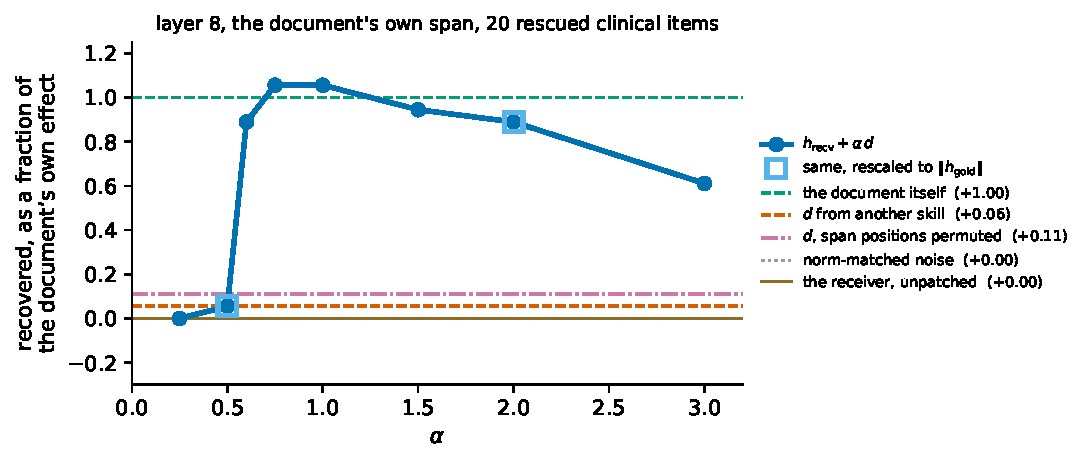
\includegraphics[width=0.9\textwidth]{fig-dose-medcalc.pdf}
\caption{Dose response of the content injection over the document's own span,
layer 8, with its controls. Open squares are the same dose rescaled per position
to the with-document norm; they coincide with the plain arms. Before the
instrument fix; the post-fix dose sweep and norm comparison are in
Appendix~\ref{app:madeof}. The horizontal lines are the three controls and the two
baselines.}
\label{fig:dose}
\end{figure*}

\begin{figure*}[tbp]
\centering
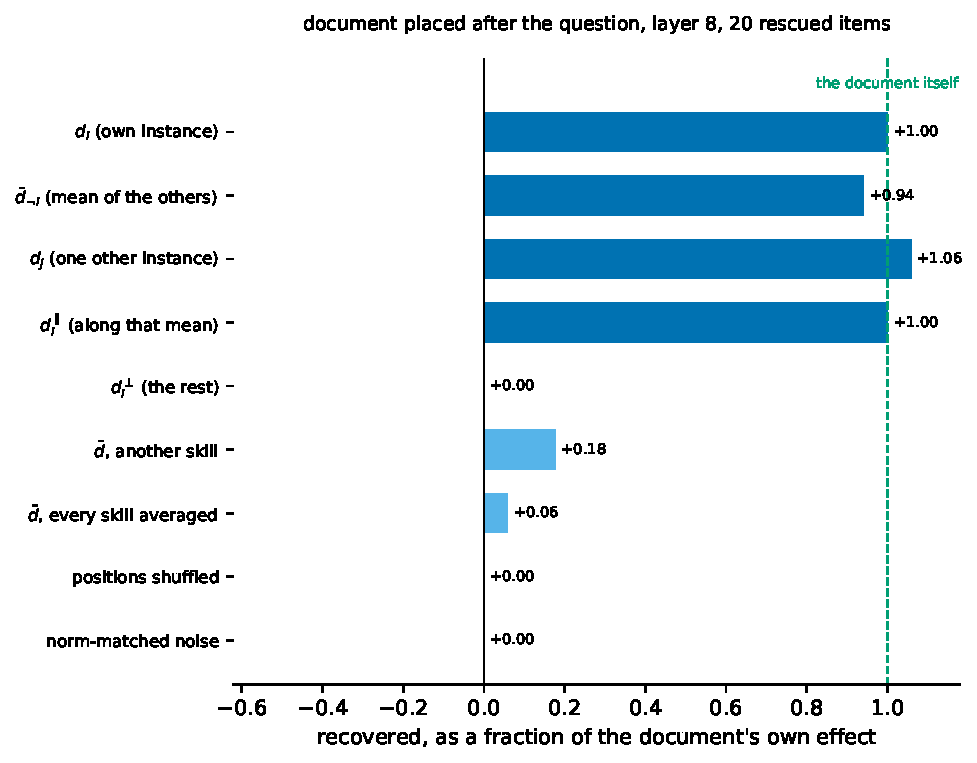
\includegraphics[width=0.72\textwidth]{fig-skilltask-medcalc.pdf}
\caption{What the content vector contains once it is able to contain the task.
Document placed after the question, layer 8, Qwen3-8B, the $40$ rescued items,
plotted as the fraction $\rho$ of Eq.~\ref{eq:rho}, before the instrument fix
(post-fix numbers in Appendix~\ref{app:madeof}). Exact accuracies and
intervals are in Table~\ref{tab:skilltask}, Appendix~\ref{app:tables}.}
\label{fig:skilltask}
\end{figure*}

\begin{figure*}[tbp]
\centering
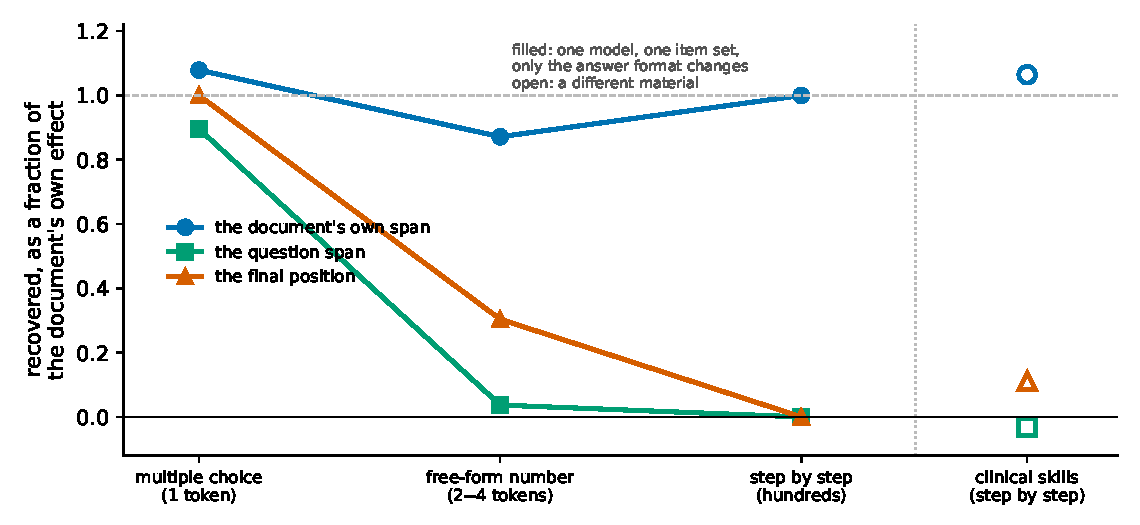
\includegraphics[width=0.92\textwidth]{fig-ladder.pdf}
\caption{What each transplant channel recovers, as a fraction of what the
document itself is worth in that setting, against how many tokens the answer
occupies. Filled markers joined by lines are one model, one item set and one
document with only the answer format changed; the clinical results are open and
deliberately not joined, because that material changes the skill, the task and
the prompt length at once. Plotting fractions rather than raw accuracies is
necessary here: the four settings have donors at $0.550$, $0.467$, $1.000$ and
$0.950$, and comparing raw numbers across them is how an earlier draft came to
report that a \emph{longer} answer made the document-span channel stronger. The
document's own span is flat at $1.00$ across every answer format. The other two
channels collapse as the answer lengthens, and the clinical points land where
the step-by-step column says they should.}
\label{fig:ladder}
\end{figure*}
\subsection{What the carrying vector is made of, in full}
\label{app:madeof}

The vector at the document's span reproduces the document's whole effect, so
what it is composed of is answerable rather than speculative. Four
decompositions, all at layer 8. \textbf{Unless marked ``after the fix'', the
numbers in this subsection come from the ten-calculator development runs made
before the instrument fix}, read against the receiver's $0.175$ and the
document's $0.950$; where a rerun exists it is given and takes precedence.

\paragraph{Not a common shift.} Averaging $\dvec$ over \emph{every} skill in the
set and writing that average gives $\rho = 0.11$, against $1.06$ for the
document's own. What makes this sharp rather than merely negative
is how much of the vector that average is: measured against the same fixed
control, two skills' content vectors have cosine $0.48$--$0.56$ at every depth,
the cosine to the all-skill mean is $0.72$--$0.76$, and $54$--$60\%$ of each
$\dvec$'s energy lies along that mean (Table~\ref{tab:geometry}). \emph{More than
half of the content vector points in a direction that carries nothing.} This is
the span-level counterpart of $\gvec$'s flat $0.098$ at
the final position in \S\ref{sec:decomp}: presence is not what acts, in either
place.

\paragraph{Not a magnitude.} The informative test is the dose curve against its
norm-matched twin. At $\alpha = 2$ the patched state is $2h_{\text{skill}} -
h_{\text{recv}}$, which is $1.76\times$ as long as the with-document state at
layer 8; rescaling it per position back to $\|h_{\text{skill}}\|$ is a $43\%$
change and costs nothing---$\rho = 0.89$ either way. At $\alpha = 0.5$ the state
is $0.88\times$ and rescaling is likewise free ($0.06$ both).

We also ran the reverse, rescaling the with-document states down to the
\emph{receiver's} norm, and it changes nothing ($\rho = 1.06$)---but that arm is
uninformative and we report it only to say so: the two norms differ by $3.5\%$ at
layer 8, so it is barely a manipulation. The $\alpha = 2$ comparison is the one
that carries the claim. The dose curve and its norm-matched twin coincide
at every $\alpha$ we ran ($0.5$: $0.350$ vs $0.350$; $2$: $0.875$ vs $0.875$;
$3$: $0.675$ vs $0.650$). The document's effect is carried by the direction its
span states point in and not by how far along it they go. Norm-matched Gaussian
noise, correspondingly, gives $0.100$, below the receiver.
The norm arms were not rerun after the fix. (The arm listed next to the
transplant in Table~\ref{tab:big40}, $0.73$, is not a norm manipulation: it is
the transfer test's paired control, the document's own $\dvec$ written over only
the prefix another skill's document shares.)

\paragraph{Graded in $\alpha$, and the transition is a step.} After the fix,
on the ten development calculators ($n=16$), $\alpha = 0.4, 0.5, 0.55, 0.6, 0.7,
1, 2$ give $\rho = 0.06, 0.00, 0.06, 0.62, 0.94, 1.00, 0.81$: at the receiver up
to $0.55$ and at the document by $0.7$. Before the fix the same sweep read
$0.17, 0.03, 0.17, 0.88, 0.97, 1.00$ ($n=30$ under a looser restriction), and an
earlier receiver gave $-0.14, +1.03, +1.03, +0.86$ at $\alpha = 0.5, 0.75, 1, 2$
(Figure~\ref{fig:dose}, pre-fix): half the content is no better than none of
it, while three quarters is already most of the effect. Past $\alpha=1$ the
recovery decays slowly rather than breaking, and against the other receiver,
where the fine grid was run, it decays the same way with the norm held fixed
($\alpha=2$: $0.875$ plain against $0.875$ rescaled; $\alpha=3$: $0.675$ against
$0.650$), so what overshooting costs is not the size of the state.

\paragraph{Localised, and in the section one would guess.} Writing $\dvec$ over
only part of the span localises the effect within the document without changing
a single prompt token---the length, the positions and the rotary phases are all
untouched, and only which states are overwritten changes. By halves (pre-fix),
the first gives $\rho = 1.06$ and the second $0.28$, and the first half agrees
with the whole span item by item on $18$ of $20$. By quarters:
\begin{center}
\resizebox{\columnwidth}{!}{%
\begin{tabular}{@{}lccccc@{}}
\toprule
quarter of the span & $n$ & 1st & \textbf{2nd} & 3rd & 4th \\
\midrule
forty calculators, after the fix & $60$ & $0.12$ & $\mathbf{0.56}$ & $0.12$ & $0.12$ \\
ten calculators, after the fix & $16$ & $0.12$ & $\mathbf{0.81}$ & $0.06$ & $0.06$ \\
ten calculators, before the fix & $20$ & $0.28$ & $\mathbf{0.83}$ & $0.11$ & $0.44$ \\
\midrule
controls on the same forty (Table~\ref{tab:big40}) & $60$ & \multicolumn{4}{c}{half dose $0.06$, permuted $0.08$, noise $0.10$} \\
\bottomrule
\end{tabular}}
\end{center}

These documents make that interpretable, because all ten have the same section
order: title, \emph{Required Inputs}, \emph{Computation} (sometimes preceded by a
\emph{Unit Conversion}), \emph{Calculation Tool}, \emph{Example}. Measured in the
units the intervention actually uses---token positions within the span, not
characters---the computational section's \emph{heading} falls at $0.18$--$0.42$
of the span, \emph{Calculation Tool} at $0.47$--$0.70$, and \emph{Example} at
$0.61$--$0.79$. So the second quarter is the \emph{body} of the computational
section, the formula itself, for every one of the ten; the first quarter is the
title, the input list and at most the opening of that section; the third is a
Python function signature and the start of a worked example; the fourth is the
rest of the example.

Read that way the procedural core carries most of the effect, and every other
quarter alone is at the control floor. Two things changed with the fix and the
larger set. The worked example, which read $0.44$ before the fix, reads $0.06$
and $0.12$ after it: \emph{we withdraw the earlier statement that it carries
about half as much as the formula.} And the formula alone, $0.81$ on ten
calculators, is $0.56$ on forty against the whole document's $0.87$, so on the
larger set the other three quarters matter in combination although none matters
alone. The boundaries are approximate and vary by calculator, so we report the
quarters and the section map rather than claiming an exact alignment.

Permuting the span's own positions, which preserves the multiset of vectors and
destroys only the correspondence between them and the tokens, gives $0.08$ on
forty calculators after the fix ($0.21$ before it): nearly all of the effect is
in that correspondence.



\paragraph{Task information, when the vector is allowed to have any.} Under the
prompt format used everywhere else in this paper the question does not arise:
the document precedes the question, so its states are a function of the document
alone and we verified that they agree across a skill's instances (bit for bit at
equal prompt length, cosine $\ge 0.997$ otherwise).
To ask what happens when the vector \emph{can} carry the task, we move the
document behind the question, keeping the answer-format instruction last, and
pad each instance's question with filler tokens so that the document begins at
the same absolute index for every instance of a skill---without which a donor
from another instance would be written at the wrong rotary phase, the error
described in \S\ref{sec:battery}. The format costs almost nothing behaviourally
(the document is worth $0.025 \to 0.925$ instead of $0.025 \to 0.950$) and it
raises the receiver's own baseline to $0.350$.

In that format the vector \emph{can} carry the task, and at layer 8 it does not
use it (read, like everything else here, on the calculators a wrong document
never rescues). After the fix ($n=28$, seven calculators) the instance's own
vector recovers $\rho = 1.00$, the mean of the skill's other instances' vectors
$1.00$, a single other instance's vector $0.96$, and the
orthogonal remainder---everything specific to this patient note---$0.04$. Before
the fix (Figure~\ref{fig:skilltask}) the same arms read $1.00$, $1.00$, $1.06$
and $0.00$. At layer $16$ the picture changes: the instance's own vector still
recovers $0.85$, but the mean of the other instances' vectors $0.63$ and a
single other instance's $0.48$, while the remainder alone stays at $0.04$. By
layer $16$ the doc-last span holds something of the question that other
instances' vectors lack and the remainder cannot supply on its own.

The geometry agrees and says why, before any injection: the cosine between two
instances' $\dvec$ in this format is $0.998$ at layer 0, $0.984$ at layer 8 and
$0.914$ by layer 32, with the fraction of energy along the instance-mean falling
from $0.997$ to $0.880$. At layer 8 the vector is $98\%$ shared, so there is
almost no instance-specific part to use; whether the remaining $12\%$ at layer 32
ever matters is a question we can pose but have not answered.

Everything else replicates across the two prompt orders (pre-fix). Another skill's vector
recovers $0.18$, the mean over every skill $0.06$, the same vectors with the
span's positions permuted $0.00$ and norm-matched noise $0.00$; rescaling to the
receiver's own norm costs nothing ($0.99$); and the first half of the span
carries $1.05$ against the second half's $0.43$, the same concentration in the
formula that the document-first format shows.



\paragraph{Where the document sits changes how deep the handover reaches.}\label{sec:whose:docklast}
Placing the document after the question moves the cliff. We first reported this
as a confirmed rank prediction, on the grounds that the doc-last span's
participation ratio past layer 16 read $28$--$33$ against the doc-first format's
$14$--$17$; \S\ref{sec:depth} shows that both of those numbers are massive
activations rather than representations, and once they are excluded the two
formats have the same, flat dimensionality. The behavioural difference is real
and the rank explanation for it is withdrawn.

The difference is large. On the same items, before the fix, as a fraction of
each format's own range:
\begin{center}
\resizebox{\columnwidth}{!}{%
\begin{tabular}{@{}lccccc@{}}
\toprule
layer & 0 & 4 & 8 & 12 & \textbf{16} \\
\midrule
document first & $1.00$ & $1.07$ & $1.14$ & $1.00$ & $\mathbf{0.14}$ \\
document last  & $0.99$ & $1.11$ & $1.00$ & $0.93$ & $\mathbf{0.80}$ \\
\bottomrule
\end{tabular}}
\end{center}

Both formats carry the document's whole effect through layer 12. At layer 16 the
document-first format carries a seventh of it and the document-last format four
fifths; the latter's own cliff comes later, between layers 16 and 20 ($0.82$ to
$0.35$). Under causal masking a document placed first cannot see the question
and a document placed last can, so the doc-last span's states are already
question-conditioned when they are captured---which is the obvious candidate
explanation, and is not one we have tested.

After the fix the layer-$16$ contrast holds: $0.85$ with the document last
($n=28$) against $0.19$ with it first on forty calculators. Before the fix, at
layers $0, 12, 16, 20$ in the document-last format the mean of the skill's other
instances tracked the instance's own ($1.06/1.00$, $0.88/0.94$, $0.82/0.82$,
$0.29/0.35$) with the remainder at the receiver; the rerun at layer $16$
($0.63$ against $0.85$, above) does not reproduce that agreement, so we no longer
claim that the instance-specific part never matters at depth---only that it does
nothing alone.

What this rules out is the reading in which the handover depth is a fixed
property of the network: it moves under a change to the prompt that leaves the
model, the document and the items alone.

\subsection{Depth, sufficiency and necessity, in full}
\label{app:depth}

\begin{table*}[tbp]
\caption{Centred participation ratio of the content matrix across the
document's span on Qwen3-8B, measured four ways, medians over $96$ items from
all $48$ documents (the plain column is bimodal, so its mean describes no
item). The first column is the quantity usually reported and the only one that
collapses. The last two columns say why---they are properties of the state
itself, not of the difference: at layer $16$ one token in $35$ of $48$
documents acquires a state $153$ times (median) the span's norm, carried by two
fixed hidden dimensions, and the top eight dimensions then hold $98\%$ of the
variance. Removing four positions out of four hundred, or normalising each
position to unit length, removes the collapse entirely.}
\label{tab:prdiag}
\centering
\small
\setlength{\tabcolsep}{4pt}
\begin{tabular}{@{}rrrrrrr@{}}
\toprule
& \multicolumn{4}{c}{participation ratio, computed\ldots} & \multicolumn{2}{c}{massive activations} \\
\cmidrule(lr){2-5}\cmidrule(l){6-7}
layer & as usual & drop 4 loud & unit-norm. & drop 8 dims & $\max/\mathrm{med}\,\|h\|$ & top-8 var. \\
\midrule
$8$ & $97.7$ & $97.0$ & $103.4$ & $114.2$ & $1.5$ & $4.9\%$ \\
$12$ & $68.1$ & $70.0$ & $79.4$ & $88.9$ & $1.6$ & $5.6\%$ \\
$14$ & $76.3$ & $76.8$ & $83.7$ & $93.7$ & $1.6$ & $5.3\%$ \\
$16$ & $1.0$ & $85.2$ & $91.4$ & $36.6$ & $152.7$ & $97.7\%$ \\
$20$ & $1.1$ & $84.9$ & $89.1$ & $70.1$ & $94.2$ & $94.8\%$ \\
$28$ & $2.5$ & $62.4$ & $70.9$ & $100.8$ & $27.2$ & $64.7\%$ \\
$34$ & $32.4$ & $34.2$ & $43.0$ & $113.4$ & $1.3$ & $15.7\%$ \\
\bottomrule
\end{tabular}

\end{table*}


On the clinical material the two questions---\emph{can} the document's states be
handed over at layer $L$, and \emph{is} the model still reading them at layer
$L$---give different answers, and the disagreement is the informative part.

Sufficiency, on forty calculators after the instrument fix ($n=60$, twenty
calculators after the restriction): a single layer's worth of the span reproduces
$\rho = 1.04, 0.94, 0.85, 0.77$ at layers $0, 4, 8, 12$ and then
$0.28, 0.19, 0.19, 0.15$ at $14, 15, 16, 20$. The first, pre-fix sweep on twenty
items (Table~\ref{tab:realspandepth}) has the same shape: $1.00$ at $0$ and $12$,
three quarters at $13$--$14$, $0.14$ at $15$ and $16$, nothing by $24$.

Necessity, from cumulative attention knockout with the full chain of thought
decoded ($n=40$ rescued items, twenty calculators): masking every position's
attention to the document's tokens from layer $L$ to the end leaves
$0.08$--$0.15$ of the items correct for every $L \le 20$ except $L=4$ ($0.33$),
then $0.38$ at $24$, $0.75$ at $28$ and $0.95$ at $32$. An earlier knockout run
capped generation at 400 tokens, truncating the chain of thought so that even the
unmasked prompt scored $0.50$; it is superseded and not used. The model is still
reading the document long after a single-layer handover has stopped working.

\paragraph{It is not that one layer is too few: the channel closes.} The
natural reading of the cliff is that a single layer stops being enough, since
writing the span at \emph{every} layer at once still recovers $0.950$. It is
wrong, and one experiment separates the two. We write the span at every layer in
a window $[\ell_{\text{lo}}, \ell_{\text{hi}}]$ and nowhere else.
The complete corrected window run uses a different receiver from the span
battery. Using its own baselines and group screen retains $222$ items from
$21$ calculators. Recovery is $0.95$ for $8$--$11$, $0.81$ for $12$--$15$,
$0.22$ for $14$--$19$ and $0.10$ for $16$--$35$, with an exact identity
control at $0.00$. The final window matches layer $16$ alone. Earlier versions
incorrectly merged this run with the span battery's receiver baselines,
producing $n=137$ and incompatible normalisation; those estimates are
superseded. Repeating the injection across late layers does not restore the
early-window recovery, although the window and single-layer sweeps are not
directly paired across receivers.

This is worth stating as a negative constraint on any mechanism, including the
one we tried to give it. Whatever ends at layer $15$ is not a capacity that more
depth can compensate for.

\paragraph{The span's representation does \emph{not} become a summary, and the
measurement that says it does is an artefact.} The obvious explanation for the
cliff is that the span has by then been compressed, and the obvious measurement
agrees: the centred participation ratio of the span's states, which counts the
directions its positions differ in, reads $64$ at layer $12$ and $17$ at layer
$16$---the same interval. We report it here because we believed it, built a
mechanism on it, and it is wrong.

Three things give it away. It is a step and not a slope: the span states'
participation ratio lies between $47$ and $75$ for every item at layer $14$ and
below $5$ for thirty-four of forty at layer $16$ (Table~\ref{tab:prdiag}), and
the content matrix's mean of $17$ at layer $16$ describes no item---thirty-two
of forty read below $5$ and the other eight at $81$. A participation ratio of
$1.0$ over four hundred positions asserts that the centred span is rank one,
which is not a statement one can make about four hundred tokens of text that
the model still has to continue. And the collapse is absent in Qwen3-0.6B and
Qwen3-1.7B at every depth ($45$--$99$, no item below $5$) although their
transplant cliff is in the same place in relative depth
(\S\ref{sec:ladder}).

The cause is measurable and known. At layer $16$---and at no earlier layer---one
token in $34$ of $40$ documents acquires a state whose norm is $99$ to $180$ times the
span's median, carried by hidden dimensions $2276$ and $676$, the same two in
all $34$. That is the massive-activation phenomenon of
\citet{sun2024massive}, which appears at a single layer per model family
\citep{shi2026melayer}; in this model the loud token is a late delimiter inside
the document rather than the sequence start. A centred spectrum is then owned by
that one position: the top eight dimensions hold $97.7\%$ of the variance at
layer $16$ against $5.4\%$ at layer $14$. Removing the four loudest positions
out of four hundred restores the participation ratio to $66$; unit-normalising
each position restores it to $68$; removing the top eight dimensions gives $27$.
Measured any of those three ways, the span's dimensionality is
\emph{flat} from layer $0$ to layer $28$ and only falls in the last few layers
(Table~\ref{tab:prdiag}).

So the honest statement is the narrower one. The single-layer handover dies
between layers $14$ and $16$; the document's representation does not lose
dimensionality there; we do not know what it does lose. What \S\ref{sec:rank}
establishes is a different and still causal fact---how many directions the
injected object needs---and in the small pre-fix repeats at layers $12$ and
$16$ that number is not lower either (Appendix~\ref{app:rank2}).



\paragraph{A warning about participation ratio on residual streams.} Effective
rank, participation ratio and intrinsic dimension are routinely computed on
residual-stream activations, including in work that reports collapses with depth
\citep{fernando2026residualspectral, sarkar2026causaldim}. Massive activations
begin at a fixed layer, are carried by a handful of dimensions at a handful of
positions, and are large enough to own a spectrum by themselves. Any such
measurement that does not exclude them will report a collapse at exactly the
emergence layer whether or not the representation has changed. Our own draft did.
We recommend reporting the per-position norm ratio alongside any spectral
statistic; here its median goes from $1.6$ to $150$ across the layer in question.
\subsection{Where in the network the content is readable, in full}
\label{app:where}

Transplanting one group of positions from the with-document forward into the
without-document forward asks where the content can be \emph{read from}; masking
attention to the document asks where it is still being \emph{read}. In the
multiple-choice format the first question gives three windows that hand off
cleanly (Figure~\ref{fig:windows}, Appendix~\ref{app:decomp}): the document's own
688 tokens work at layers 0--10 and fall off a cliff at 11, the question's 42--47
tokens work at 11--16, and the final prompt position works at 21--27. The handoff
is not an artefact of a shared analysis---the two experiments were run
independently---and at layer 11 the document-span channel drops from $0.308$ to
$0.128$ while the question-span channel rises from $0.231$ to $0.308$. The
windows survive a change of model and not a change of format
(Table~\ref{tab:windows2}): in free-form, on the same model and items, the
question span recovers $0.000$--$0.025$ at every one of 12 layers.

The second question gives a different shape. No single pathway is necessary:
masking only the final position's attention to the document costs nothing
($0.436$ against $0.436$) and masking only the question span's leaves $0.282$,
so the read is redundantly distributed, as \citet{jit2025taskrepr} report for
task representations generally. What is necessary is the document's own tokens.
On third-party skills, making them unattendable for the whole forward takes
accuracy from $0.550$ $[0.400, 0.700]$ to $0.075$ $[0.000, 0.175]$, against
$0.025$ $[0.000, 0.075]$ with no document in the prompt at all---ninety per cent
of the benefit, with the remainder inside the no-document interval. Masking an
equal-length span of the patient note instead costs less, $0.150$
$[0.050, 0.275]$. A genuinely inert length-matched control cannot be built here,
since the only other long span is the data the task needs, so this bounds
``removing 900 tokens'' loosely but in the right direction.

Single-layer knockouts measure nothing on a 688-token span, because a layer
denied the read recovers it one layer later; cumulative knockouts are required
and are what we report. Cumulatively, the document stops being needed at layer
22 of 28 when the answer is one token, and is still being read at $83\%$ depth
when the answer is several hundred---the necessity-side view of
\S\ref{sec:onepos}.



\subsection{What the content component belongs to, in full}
\label{app:whose}
\label{app:belongs}

If $\dvec$ were a ``skill vector'' it would be reusable: extracted from one task
it would work on another. Its \emph{direction} is reusable. Its \emph{effect}
is not, and the gap between those two statements is the finding.

\paragraph{The vector that carries contains no task information, and we check
rather than argue it.} Everything in this section so far is about the vector at
the final position, the one that does not act. The vector that does act---the
content component over the document's own span---has a property that makes the
question sharp. In the prompt format the behavioural runs use, the document
precedes the question, so causal masking makes the document's hidden states a
function of the system text and the document alone. Within one skill the
document is byte-identical across its instances, so $\dvec(\text{span})$ should
be \emph{the same tensor} for every instance of that skill.

It is. Across the ten calculators in the causal set, the document span occupies
token positions $43$ to $43+m$ in every prompt, the token ids there are
pairwise identical across instances (zero differing positions in $40$ notes),
and truncating two prompts to the end of the span and re-running the forward
gives a relative difference of $0.0$. In the full prompts the states differ by a
relative $3.5\times10^{-3}$ at layer 0 and $8.6\times10^{-3}$ at layer 8, with
zero positions below cosine $0.999$---accumulated bf16 rounding from the
differing sequence lengths, not content. The decode arms show the same thing
behaviourally: the mean of the \emph{other} instances' vectors and the
instance's own agree to three decimals at every running mean, and the component
of $\dvec_i$ orthogonal to that mean lands exactly on the receiver's baseline.

So the vector that reproduces the document's entire effect is a function of the
document and of nothing else. Whatever a ``skill vector'' should be, this one is
not a joint encoding of skill and task; it is the skill, and it is sufficient.
The complementary experiment---moving the document behind the question so that
its states \emph{can} see the task---is \S\ref{sec:whose:docklast}.

\paragraph{The direction differs by skill; the effect does not transfer.}
On the clinical material each skill has 20 instances, so ``same skill, different
task'' is directly measurable. Content vectors from different patient notes under
the same calculator have cosine $0.789$ at layer 20 and $0.876$ at layer 30;
vectors from different calculators, $0.320$ and $0.653$ ($n=40$, Qwen3-8B). On
the synthetic tier the analogous split is by conversion family, $0.869$ within
against $0.705$ across at the last layer. The direction of $\dvec$ carries the
identity of the document, increasingly so with depth. Its effect at the final
position does not: injecting the mean direction $\bar{\dvec}$, or another item's
$\dvec_j$, repairs $0.000$ at every one of 16 layers in the free-form format
against $0.268$ for the item's own, and in multiple choice reaches $0.098$,
$0.293$ and $0.049$ for the mean, a same-family and a different-family donor
against $0.780$ for $\dvec_i$ (Table~\ref{tab:causal}). The one band where a
donor looks transferable is the band \S\ref{sec:traps} identifies independently
as one where the forward pass is damaged and every condition rises together.

\paragraph{Nothing about it distinguishes rescued items from persistent
failures.} The norms and angles of $\dvec$ and $\gvec$ agree to three digits
across the two cells (layer 30, 8B, real skills: $\|\dvec\|$ $189.4$ vs $185.4$,
$\cos(\dvec,\gvec)$ $-0.469$ vs $-0.468$). A representational-similarity measure
over the question span does separate them under the gold skill at layers 10--16
($-0.0037$ to $-0.0070$, non-overlapping intervals, $n=150+150$)---and separates
them just as much under a length-matched \emph{wrong} skill ($-0.0035$ to
$-0.0056$). Zero layers pass a control the design required in advance, so what
looked like a signature of ``the skill worked here'' is a signature of ``a
document is present'': \S\ref{app:geometry}'s trap one register down, and the
reason we report a causal channel rather than a similarity score.

\paragraph{The content component's size depends on where it is written.} At the
final position the content component is a $6\%$ perturbation of the state it
displaces at layer 6 ($\|\dvec\|=2.3$ against $\|h_{\text{no}}\|=37.3$), rising
to $51\%$ by layer 35---and it is causally inert at every one of them. Over the
document's own span the same difference of the same two conditions is $95\%$ to
$115\%$ of the state at every depth (Table~\ref{tab:geometry})---a replacement
rather than a nudge---and it is causally complete (\S\ref{sec:battery}). What
distinguishes the two places is not how much the document is written into them;
it is whether what is written is the whole of what the downstream computation
reads.

\paragraph{The shared part carries the norm, not the effect.} Between $73\%$ and $99.7\%$ of each item's
$\dvec_i$ lies along the shared mean direction, depending on layer
(Table~\ref{tab:geometry-tierA}); the remainder occupies an effective 3--18 dimensions
out of 2048--4096. The reusable part is almost all of the norm and, in free-form
answering, none of the effect; in multiple choice it is worth $0.06$ of the
$0.79$ the item's own vector achieves. A single vector per skill is therefore a
fair description of
what the injection \emph{looks like} and a wrong description of what it
\emph{does}, which is the same inversion as \S\ref{app:geometry} one level
down.




  % Appendix -- rank truncation, the model ladder and cross-task replication.
\section{Rank truncation, the model ladder and replication}
\label{app:scale}

\begin{table*}[tbp]
\caption{The channel and the truncation curve at three model widths, each with
its own restricted split and its own injection layer at matched relative depth.
$\rho$ is Eq.~\ref{eq:rho}; \emph{gold} is what the document itself is worth on
that model's restricted items, which is why the $0.6$B and $1.7$B rows have low
absolute accuracy and a large $n$: those models solve almost nothing without the
document, so almost every item qualifies. Qwen3-0.6B and Qwen3-8B are after the
instrument fix; Qwen3-1.7B is before it, and its curve is not monotone, so its
$k^{*}$ is not interpretable. $k^{*}$ sits between $32$ and $64$ at $d=1024$
and at $d=4096$ alike; a width-proportional account predicts $k\approx12$ for
the first. Mistral-7B is in Table~\ref{tab:replicationfull}.}
\label{tab:laddermodels}
\centering
\footnotesize
\setlength{\tabcolsep}{3pt}
\begin{tabular}{@{}lrrrrrrrrrrrr@{}}
\toprule
model & $d$ & layers & inject & $n$ & gold & $\rho$(full) & $k{=}16$ & $32$ & $64$ & $128$ & bottom-$64$ & $k^{*}$ \\
\midrule
Qwen3-0.6B & $1024$ & $28$ & $6$ & $204$ & $0.260$ & $+0.83$ & $+0.02$ & $+0.23$ & $+0.81$ & $+0.85$ & $+0.02$ & $41$ \\
Qwen3-1.7B & $2048$ & $28$ & $6$ & $267$ & $0.090$ & $+0.54$ & $+0.33$ & $+0.50$ & $+0.42$ & $+0.29$ & $+0.12$ & $23$ \\
Qwen3-8B & $4096$ & $36$ & $8$ & $135$ & $0.919$ & $+0.89$ & $+0.05$ & $+0.12$ & $+0.63$ & $+0.77$ & $+0.03$ & $47$ \\
\bottomrule
\end{tabular}

\end{table*}

\subsection{Rank truncation and the model ladder, in more detail}
\label{app:rank2}

On the denser grid every rank curve in the paper reaches its untruncated value:
the three TheoremQA rows at $k=192$--$384$ ($0.806$/$0.882$/$0.871$ against
$0.839$ for Qwen3-8B, $0.717$/$0.701$/$0.732$ against $0.740$ for Qwen3-0.6B,
and $0.819$/$0.880$/$0.819$ against $0.940$ for Mistral-7B at $k=192,256,384$),
MedCalc with Qwen3-8B and Qwen3-0.6B at $k=256$, and MedCalc with Mistral-7B at
$k=384$ ($0.842$, exactly its untruncated value; $0.825$ at $512$). The knee
$k^{*}$ is computed on the fixed grid $\{16,32,64,128\}$ and is unchanged by
the added points, by construction.

Every measurement so far says \emph{where} the document's effect lives. This one
says \emph{how big it is}, in the only unit that is comparable across the
task-vector literature: the number of directions of the injected object that the
model actually uses.

We truncate the content matrix across the span's positions to rank $k$ before
writing it. With $\dvec \in \mathbb{R}^{m \times D}$ and $\bar{\dvec}$ its mean
over positions,
\begin{equation}
\dvec^{(k)} \;=\; \bar{\dvec} \;+\; \sum_{i=1}^{k} \sigma_i u_i v_i^{\top},
\qquad
\dvec - \bar{\dvec} \;=\; \textstyle\sum_i \sigma_i u_i v_i^{\top},
\end{equation}
the mean kept and only the variation truncated, so that $k$ is comparable with a
centred participation ratio. $k=1$ is the closest thing in this setting to a
task vector: one direction, applied at every position of the span.

One direction is not enough, and neither are sixteen
(Figure~\ref{fig:rank}). On the full rerun's screened subset after the fix
($n=135$, $14$ calculators), recovery
at layer $8$ is $0.07, 0.05, 0.12, 0.63, 0.77$ at $k = 4, 16, 32, 64, 128$
against $0.89$ untruncated, and half of the curve's range above $k=16$ is
recovered at $k^{*}=47$ ($95\%$ bootstrap interval over calculators $[43, 55]$;
interpolated in $\log_2 k$, the definition fixed before the model ladder ran).
The ten-calculator development curve, before the fix, reads
$0.11, 0.06, 0.06, 0.11, 0.11, 0.33, 0.72, 0.94$ at $k = 1,2,4,8,16,32,64,128$
and gives $k^{*}=45$.

$k^{*}$ is anchored to the largest value on the grid $k \le 128$, not to the
untruncated transplant. Where $k=128$ is close to untruncated (Qwen3-8B, $0.77$
against $0.89$) that makes little difference; where it is not (Mistral-7B,
$0.71$ against $0.92$) the knee is bounded by the grid, and a finer or longer
grid could move it up.

\paragraph{It is the top of the spectrum, not the count.} Keeping the
\emph{bottom} $k$ singular directions instead---the same rank, the discarded
half of the spectrum---gives $\rho = 0.06$ at $k=16$ and $0.00$ at $k=64$ on
forty calculators ($0.00$ and $0.06$ on the development set), both at the
receiver. Without that control, ``sixty-four directions are enough'' could not
be distinguished from ``any sixty-four directions will do''.

\paragraph{The requirement does not fall with depth (pre-fix, small $n$).} If
the handover died at layer $15$ because the object had shrunk, the number of
directions needed would shrink with it. Repeating the truncation where the
transplant still works, on the calculators the receiver never solves, gives
accuracy $0.00$ at $k=16$ and $0.62$ at $k=128$ against $1.00$ untruncated at
layer $12$ ($n=16$), and $0.25$ at $k=16$ and $0.71$ at $k=128$ against $0.79$ at
layer $16$ with the document after the question ($n=28$)---the knee between $64$
and $128$ in both. These runs predate the fix and are small; we read them as
``not lower'', not as a measured knee. At layer $16$ with the document \emph{before} the question, where the
transplant is already at the floor ($\rho=0.06$), there is no curve at all:
every truncation reads between $0.00$ and $0.06$, because there is no longer an
effect for truncation to remove. We do not read the rank of the layer-$16$
doc-first object at all, since that is the layer at which the massive
activations of \S\ref{sec:depth} take over its spectrum.



\paragraph{The obvious converse does not work, and we report that.} If a deep
layer's handover failed for want of directions, supplying it with a higher-rank
message should restore it. We tried the direct version---write the layer-8
donor into layer 16---on ten calculators ($n=30$ after restricting to items that
neither the wrong document nor the no-document prompt solves). It does not
restore; it reads $\rho = 0.00$ where the same-layer donor reads $0.06$,
and matching the norm to layer 16's scale recovers only part of the gap
($0.13$). The layer-8 state is not a high-rank version of the layer-16 state, it
is a different code, and the transfer is directional:
\citet{ardoin2026promptcompression} find middle-to-early injection optimal, and
we find early-to-middle injection harmful.
\subsection{Replication across tasks and model families, in full}
\label{app:replication}

Every point behind Table~\ref{tab:replication}. All runs are after the
instrument fix. MedCalc rows use forty calculators and each model's own
behavioural screen; TheoremQA rows use SRA-Bench's $747$ questions with its
prompt and scorer verbatim, and since most of its $320$ skills serve a single
question the receiver screen is per skill group, and reduces to an item-level screen for singleton skills.
Those $747$ questions are the pool each TheoremQA run samples from, not the set
it evaluates: a run takes at most four questions per skill and at most two
hundred skills, which here is $142$--$168$ items over $113$--$122$ skills before
the screen. The MedCalc rows are not sampled this way, and the two should not be
read as equally exhaustive. Knockout rows are fractions of each
model's rescued items kept when attention to the document is blocked from layer
$L$ to the end, unrestricted.

\begin{table*}[tbp]
\caption{The replication curves. Battery, sufficiency and rank are $\rho$
(Eq.~\ref{eq:rho}) on the restricted split; necessity is the fraction of rescued
items kept. ``Another family'' (MedCalc) and ``another skill'' (TheoremQA) are
the transfer controls available in each set.}
\label{tab:replicationfull}
\centering
\scriptsize
\setlength{\tabcolsep}{3pt}
\begin{tabular}{@{}p{0.15\textwidth}p{0.22\textwidth}p{0.57\textwidth}@{}}
\toprule
task / model & measurement & values \\
\midrule
MedCalc / Qwen3-8B & battery, L8 ($n=135$, 14 groups) & transplant 0.89, own $d$ on shared prefix 0.65, $\alpha{=}0.5$ 0.04, another skill 0.05, another family 0.05, same family 0.12 ($n=41$), permuted 0.05, noise 0.02, null 0.00 \\
 & sufficiency ($n=135$) & L0 0.98, L1 0.95, L2 0.94, L3 0.96, L4 0.98, L5 0.94, L6 0.94, L7 0.92, L8 0.89, L9 0.85, L10 0.89, L11 0.81, L12 0.74, L13 0.16, L14 0.16, L15 0.06, L16 0.06, L17 0.07, L18 0.03, L19 0.02, L20 0.03, L21 0.02, L22 0.04, L23 0.03, L24 0.01, L25 0.02, L26 0.03, L27 0.03, L28 0.02, L29 0.03, L30 0.05, L31 0.04, L32 0.04, L33 0.02, L34 0.01, L35 0.00 \\
 & necessity ($n=134$ rescued, screened groups) & L0 0.03, L1 0.01, L2 0.03, L3 0.01, L4 0.04, L5 0.05, L6 0.03, L7 0.03, L8 0.04, L9 0.03, L10 0.03, L11 0.04, L12 0.04, L13 0.07, L14 0.08, L15 0.07, L16 0.07, L17 0.08, L18 0.06, L19 0.07, L20 0.12, L21 0.08, L22 0.09, L23 0.08, L24 0.25, L25 0.58, L26 0.46, L27 0.56, L28 0.57, L29 0.57, L30 0.78, L31 0.84, L32 0.85, L33 0.88, L34 0.91, L35 0.94 \\
 & rank, L8 ($n=135$) & $k{=}4$ 0.07, $k{=}16$ 0.05, $k{=}32$ 0.12, $k{=}64$ 0.63, $k{=}128$ 0.77, full 0.89, bottom-16 0.04, bottom-64 0.03, $k^{*}$ 47 \\
\midrule
TheoremQA / Qwen3-8B & battery, L8 ($n=99$, 75 groups) & transplant 0.84, own $d$ on shared prefix 0.86, $\alpha{=}0.5$ 0.19, another skill 0.25, permuted 0.24, noise 0.22, null 0.00 \\
 & sufficiency ($n=99$) & L0 1.00, L1 1.01, L2 0.98, L3 0.94, L4 0.94, L5 0.96, L6 0.95, L7 0.91, L8 0.84, L9 0.75, L10 0.82, L11 0.67, L12 0.61, L13 0.44, L14 0.37, L15 0.22, L16 0.19, L17 0.17, L18 0.19, L19 0.19, L20 0.14, L21 0.13, L22 0.09, L23 0.11, L24 0.14, L25 0.12, L26 0.16, L27 0.10, L28 0.16, L29 0.12, L30 0.09, L31 0.14, L32 0.04, L33 0.09, L34 0.08, L35 0.00 \\
 & necessity ($n=63$ rescued, screened groups) & L0 0.25, L1 0.25, L2 0.13, L3 0.19, L4 0.24, L5 0.21, L6 0.24, L7 0.25, L8 0.27, L9 0.24, L10 0.21, L11 0.24, L12 0.21, L13 0.29, L14 0.27, L15 0.19, L16 0.27, L17 0.30, L18 0.35, L19 0.43, L20 0.49, L21 0.57, L22 0.52, L23 0.63, L24 0.70, L25 0.81, L26 0.78, L27 0.81, L28 0.78, L29 0.84, L30 0.86, L31 0.90, L32 0.89, L33 0.92, L34 0.90, L35 0.98 \\
 & rank, L8 ($n=99$) & $k{=}4$ 0.17, $k{=}16$ 0.24, $k{=}32$ 0.30, $k{=}64$ 0.54, $k{=}128$ 0.67, full 0.84, bottom-16 0.10, bottom-64 0.13, $k^{*}$ 50 \\
\midrule
MedCalc / Qwen3-0.6B & battery, L6 ($n=362$, 38 groups) & transplant 0.91, own $d$ on shared prefix 0.90, $\alpha{=}0.5$ 0.07, another skill 0.30, another family 0.04, same family 0.11 ($n=204$), permuted 0.02, noise 0.03, null 0.00 \\
 & sufficiency ($n=362$) & L0 1.05, L1 1.08, L2 1.03, L3 0.97, L4 1.00, L5 1.07, L6 0.91, L7 0.91, L8 0.96, L9 0.70, L10 0.67, L11 0.23, L12 0.10, L13 0.14, L14 0.12, L15 0.18, L16 0.13, L17 0.10, L18 0.13, L19 0.12, L20 0.12, L21 0.07, L22 0.02, L23 0.05, L24 0.07, L25 0.03, L26 0.01, L27 0.00 \\
 & necessity ($n=90$ rescued, screened groups) & L0 0.03, L1 0.06, L2 0.03, L3 0.06, L4 0.04, L5 0.02, L6 0.06, L7 0.02, L8 0.06, L9 0.01, L10 0.03, L11 0.03, L12 0.00, L13 0.00, L14 0.02, L15 0.01, L16 0.02, L17 0.06, L18 0.04, L19 0.03, L20 0.03, L21 0.46, L22 0.76, L23 0.77, L24 0.84, L25 0.87, L26 0.89, L27 1.00 \\
 & rank, L6 ($n=362$) & $k{=}4$ 0.01, $k{=}16$ 0.00, $k{=}32$ 0.12, $k{=}64$ 0.79, $k{=}128$ 0.67, full 0.91, bottom-16 0.02, bottom-64 0.02, $k^{*}$ 43 \\
\midrule
TheoremQA / Qwen3-0.6B & battery, L6 ($n=132$, 97 groups) & transplant 0.74, own $d$ on shared prefix 0.57, $\alpha{=}0.5$ 0.13, another skill 0.08, permuted 0.09, noise 0.10, null 0.00 \\
 & sufficiency ($n=132$) & L0 0.97, L1 0.93, L2 0.91, L3 0.88, L4 0.88, L5 0.89, L6 0.74, L7 0.74, L8 0.69, L9 0.65, L10 0.64, L11 0.40, L12 0.33, L13 0.33, L14 0.31, L15 0.29, L16 0.28, L17 0.19, L18 0.22, L19 0.14, L20 0.13, L21 0.05, L22 0.06, L23 0.06, L24 0.03, L25 0.01, L26 0.00, L27 0.00 \\
 & necessity ($n=125$ rescued, screened groups) & L0 0.11, L1 0.13, L2 0.10, L3 0.10, L4 0.10, L5 0.06, L6 0.09, L7 0.15, L8 0.17, L9 0.14, L10 0.14, L11 0.11, L12 0.20, L13 0.18, L14 0.18, L15 0.21, L16 0.27, L17 0.25, L18 0.34, L19 0.33, L20 0.54, L21 0.66, L22 0.86, L23 0.88, L24 0.90, L25 0.96, L26 0.97, L27 0.99 \\
 & rank, L6 ($n=132$) & $k{=}4$ 0.06, $k{=}16$ 0.09, $k{=}32$ 0.14, $k{=}64$ 0.43, $k{=}128$ 0.61, full 0.74, bottom-16 0.06, bottom-64 0.08, $k^{*}$ 52 \\
\midrule
MedCalc / Mistral-7B & battery, L4 ($n=92$, 20 groups) & transplant 0.84, own $d$ on shared prefix 0.53, $\alpha{=}0.5$ 0.19, another skill 0.16, another family 0.28, same family 0.35 ($n=31$), permuted 0.16, noise 0.14, null 0.00 \\
 & sufficiency ($n=92$) & L0 0.96, L1 0.96, L2 0.89, L3 0.79, L4 0.84, L5 0.79, L6 0.75, L7 0.46, L8 0.46, L9 0.26, L10 0.21, L11 0.21, L12 0.14, L13 0.19, L14 0.23, L15 0.21, L16 0.09, L17 0.14, L18 0.25, L19 0.07, L20 0.09, L21 0.12, L22 0.09, L23 0.04, L24 0.11, L25 0.14, L26 0.11, L27 0.11, L28 0.12, L29 0.18, L30 0.09, L31 0.00 \\
 & necessity ($n=46$ rescued, screened groups) & L0 0.04, L1 0.09, L2 0.11, L3 0.20, L4 0.15, L5 0.20, L6 0.15, L7 0.15, L8 0.09, L9 0.09, L10 0.15, L11 0.09, L12 0.33, L13 0.22, L14 0.24, L15 0.24, L16 0.26, L17 0.28, L18 0.28, L19 0.28, L20 0.17, L21 0.28, L22 0.46, L23 0.41, L24 0.41, L25 0.41, L26 0.43, L27 0.50, L28 0.65, L29 0.70, L30 0.70, L31 0.85 \\
 & rank, L4 ($n=92$) & $k{=}4$ 0.16, $k{=}16$ 0.14, $k{=}32$ 0.09, $k{=}64$ 0.30, $k{=}128$ 0.54, full 0.84, bottom-16 0.11, bottom-64 0.14, $k^{*}$ 72 \\
\midrule
TheoremQA / Mistral-7B & battery, L4 ($n=115$, 94 groups) & transplant 0.94, own $d$ on shared prefix 0.80, $\alpha{=}0.5$ 0.27, another skill 0.20, permuted 0.17, noise 0.13, null 0.00 \\
 & sufficiency ($n=115$) & L0 1.01, L1 1.05, L2 0.96, L3 0.92, L4 0.94, L5 1.00, L6 0.82, L7 0.49, L8 0.42, L9 0.40, L10 0.30, L11 0.19, L12 0.11, L13 0.12, L14 0.11, L15 0.08, L16 0.06, L17 0.10, L18 0.06, L19 0.06, L20 0.05, L21 0.07, L22 0.06, L23 0.08, L24 0.06, L25 0.07, L26 0.06, L27 0.07, L28 0.10, L29 0.05, L30 0.07, L31 0.00 \\
 & necessity ($n=65$ rescued, screened groups) & L0 0.09, L1 0.05, L2 0.14, L3 0.08, L4 0.06, L5 0.05, L6 0.05, L7 0.02, L8 0.05, L9 0.05, L10 0.12, L11 0.11, L12 0.18, L13 0.34, L14 0.31, L15 0.37, L16 0.40, L17 0.40, L18 0.43, L19 0.60, L20 0.66, L21 0.80, L22 0.88, L23 0.82, L24 0.85, L25 0.89, L26 0.89, L27 0.88, L28 0.89, L29 0.91, L30 0.86, L31 0.94 \\
 & rank, L4 ($n=115$) & $k{=}4$ 0.17, $k{=}16$ 0.20, $k{=}32$ 0.23, $k{=}64$ 0.48, $k{=}128$ 0.76, full 0.94, bottom-16 0.14, bottom-64 0.13, $k^{*}$ 64 \\
\bottomrule
\end{tabular}

\end{table*}

Three observations are not in the main text. (i) On TheoremQA with Qwen3-8B,
blocking attention to the document from layer $0$ still keeps $0.31$ of the
rescued items, against $0.12$ on MedCalc. Blocking attention is not removing
the document---its positions still shift the question's rotary phase and length
---and the receiver restriction selects failures near the model's decision
boundary; we have not separated the two. (ii) The same receiver-based selection is the
most likely reason TheoremQA's controls sit at $0.19$--$0.25$ for Qwen3-8B. (iii)
On LogicBench (not shown), the method's resolution fails: with mostly binary
answers the restricted split ($n=57$, $16$ skills) gives the transplant $0.75$
$[0.60, 0.88]$, its own $\dvec$ on the shared prefix $0.80$, half a dose $0.44$, another skill
$0.38$, permuted $0.25$ and noise $0.15$, and the depth curve has no cliff
($0.93$ at layer $0$, $0.49$ at $16$, $0.33$ at $20$).

  % Appendix F -- related work in full.
\section{Related work, at length}
\label{app:related}

\paragraph{Skill benchmarks measure the effect, not the mechanism.}
A 2026 literature evaluates skill documents behaviourally: across domains
\citep{skillsbench2026}, on executable software-engineering tasks
\citep{sweskills2026}, and under different delivery protocols
\citep{skillsinjector2026}; a parallel line studies which skill to retrieve.
Closest in motivation is distilling a skill into weights
\citep{skilltolora2026}, which asks what a skill \emph{could} become rather
than what it already is at inference time. None of this work looks inside the
forward pass, and the effect sizes it reports are exactly what our
\S\ref{sec:traps} shows can be format-dependent.

\paragraph{Task and function vectors, and the two limits on what one carries.}
That a context can be compressed into a single activation-space direction is
established for in-context demonstrations \citep{hendel2023taskvectors,
todd2024functionvectors} and, in weight space, for fine-tuning
\citep{ilharco2023taskarithmetic}. Methodologically we are in this line: our
$\dvec$ is extracted and re-injected the same way. Two limits on that move are
now known, and they are not the same limit.

\citet{dong2026taskvectorlimits} prove the first. In a linear transformer,
injecting one task vector is functionally a rank-one map, so a task whose
input--output relation is high-rank---a bijection, for instance---cannot be
encoded by a single vector; they confirm it on Llama-7B/13B and repair it by
injecting several vectors at several demonstration positions. That result
\emph{explains one of ours}: on the synthetic tier, $\bar{\dvec}$---one vector
shared by the whole item set, which is what a reusable skill vector would
be---recovers $0.098$, and the mapping it would have to encode is a 39-row
lookup table. We do not claim that null as new; we attribute it.

The limit this paper is about is different, and the two can be separated
empirically. On the same synthetic tier, the \emph{item's own} $\dvec_i$
recovers $0.805$ through the same single position despite that same high-rank
mapping, because the answer is one token; and on clinical skills the same
injection recovers nothing because the answer is hundreds of tokens. Rank
constrains which mappings one vector can express; length constrains how much of
a decision any small position group can carry, whatever the mapping.
\citet{dura2026sequentialpatching} state the length limit as a motivation for
patching CoT sequentially rather than at a static position; \S\ref{sec:onepos}
turns it into a controlled measurement, and \S\ref{sec:rank} measures the rank
of the \emph{representation} rather than of the mapping.

We also differ in position. Function and task vectors are read from, and written
to, one position, and are validated on tasks whose answer is a single token.
\citet{mehrafarin2026cothidden} show how far that can be pushed and, read
against our result, show what the position holds: patching a single late
position with a state taken from the model's \emph{own completed} chain of
thought recovers the correct GSM8K answer at least $99\%$ of the time, while our
donor---taken from the prompt, before any reasoning---recovers nothing. Same
position, same intervention; what differs is whether the answer already exists
in the donor. \citet{dasilva2025steeringoff} report a reliability failure of the
same channel from another direction: across 36 models, function vectors with
default parameters recover 5-shot performance in $20\%$ of model--task pairs.

\paragraph{When one vector \emph{is} enough, and what that tells us.}
The strongest recent positive result for single-vector compression is
\citet{ardoin2026promptcompression}, who learn a weighted sum of an instruction
prompt's activations at a middle layer, inject the resulting \emph{single}
vector at one placeholder position in an early layer, and lose under two points
of accuracy. We read it as convergent rather than contradictory, for two
reasons, and both are load-bearing here. First, every task on which it succeeds
has a short answer: capitals, ISO codes, continents, years, word translation,
antonyms, currency codes---all single-word exact match---and ARC-Easy, which is
a single letter. That is exactly the half of the answer-length axis where our
own single-position patch also works ($0.805$ on the synthetic tier,
\S\ref{sec:onepos}); the half where it fails is the one their evaluation does
not enter. Second, their optimal configuration extracts at a middle layer and
injects at an \emph{early} one---their stated reason is that an early injection
leaves more layers to integrate it---which is independently the direction of our
depth result (\S\ref{sec:depth}). Taken with \citet{dong2026taskvectorlimits}
and \citet{wiegreffe2025mcq}, the three give one sentence: a single vector is a
\emph{selector} among behaviours the model already has---their appendix encodes
nine tasks in one vector, about three bits---and not a carrier of content that
needs a hundred directions to rebuild.

\paragraph{Three different objects are called ``rank'' here.} Because this paper
adds a fourth, we separate them explicitly. \citet{dong2026taskvectorlimits}
bound the rank of the \emph{task map}: which input--output relations one
injected vector can express. \citet{sarkar2026causaldim} measure the rank of the
\emph{Jacobian}, $\mathrm{eff\text{-}rank}\,\mathbb{E}_x[J_L^\top J_L]$---how
many directions of a layer causally reach the output---and report it to be
layer-intrinsic and, notably, unchanged between Gemma-2-2B and Gemma-2-9B.
\citet{fernando2026residualspectral} measure the rank of the \emph{composed
operator} across depth and find it collapses by about $65\times$ in
Llama-3.1-8B. We measure the rank of a \emph{representation}: the matrix
$\dvec\in\mathbb{R}^{m\times d}$ that one document contributes across its own
$m$ span positions. The distinction matters for what our result means. An
earlier draft combined a layer-intrinsic causal capacity
\citep{sarkar2026causaldim} with the participation ratio of $\dvec$ falling from
$64$ to $17$ to argue that the handover closes on the \emph{message} side; that
fall is massive activations (\S\ref{sec:depth}), and with them excluded the
ratio is flat, so we withdraw the argument and do not know on which side the
window closes. We are also, among these four, the only one to truncate the
injected object itself and read out behaviour; the other three use a theorem, a
first-order attribution proxy, and a spectral surgery on the weights.

A caution applies to all of the descriptive ones, ours included.
\citet{sun2024massive} document activations three orders of magnitude above the
median, carried by a fixed pair of hidden dimensions at a small set of token
positions, appearing at a single layer \citep{shi2026melayer} and acting as
bias terms. A spectral statistic computed on a residual stream past that layer
is a statistic about those activations. Our own centred participation ratio
reads $1.0$ over four hundred positions at layer $16$ of Qwen3-8B and $66$ once
four positions are dropped (\S\ref{sec:depth}); an uncentred entropy rank, which
is what \citet{fernando2026residualspectral} report collapsing by $65\times$, is
if anything more exposed, since the massive component is not removed by
centring there either. We do not claim their result is an artefact---their
object is the composed operator, not a representation---but the check is cheap
and we think it should be standard.

\paragraph{Compressing a document into parameters or into few tokens.} A
parallel line replaces the document with weights rather than activations---
hypernetworks that emit LoRA parameters from a document
\citep{doc2lora2026}, and context distillation into a knowledge module in both
output and hidden space \citep{deepcontextdistill2025}. These are orthogonal to
us in method (weights, and training, versus activations and none) but share the
premise that a document's effect is compressible.
\citet{contextreturns2026} report that re-supplying the context after such
internalisation \emph{degrades} accuracy, which is a phenomenon our
$\tvec=\gvec+\dvec$ split gives a vocabulary for: what is internalised is not
the same object as what the document contributes while present.

\paragraph{Activation patching.}
We follow the methodology literature on what patching licenses
\citep{zhang2023bestpractices, heimersheim2024patching}: transplants establish
sufficiency, knockouts necessity, and neither alone establishes a route. Two
recent results are close to ours and we read them as convergent evidence rather
than as competition. \citet{onset2025instruction} patch between minimal-contrast
prompts differing only in an instruction span and find an ``onset'' layer past
which interventions stop mattering; our layer-21 result---beyond which masking
the document is free---is the same shape of finding from the opposite direction
(knockout rather than patch) with a document rather than an instruction.
\citet{jit2025taskrepr} argue that transferable task representations are
temporally local and assembled just in time; our knockouts say the same thing
about reading a document, in that no single position group is necessary.
\citet{semanticconflicts2026} likewise localise recoverable causal signal to a
changed cue region plus a few intermediate tokens before aggregation near the
output. Mechanistic work on retrieval-augmented generation
\citep{ragcite2026} patches the residual stream to localise attribution but
does not separate presence from content.


  % Appendix G -- additional tables.
\section{Additional tables}

% These numbers are recomputed from the run outputs by
% whitebox/analysis/audit.py, which fails loudly if any of them drifts.
\begin{table*}[tbp]
\caption{Where the aggregate log-probability gap comes from, synthetic control,
layer 21, $n=39$. A cell's contribution to the mean is its size share times its
own gap, so the column adds up exactly. The mean vector beats the true state
overall because F and B---the cells where the document does not work---%
contribute $133\%$ of the gap; on R, where it does work, the true state wins by
$2.5$ nats and by $0.69$ in accuracy.}
\label{tab:cells}
\centering
\small
\begin{tabular}{lrrrrr}
\toprule
cell & $n$ & mean $-$ real (nats) & contribution to $+2.747$ & acc.\ real & acc.\ mean \\
\midrule
\textbf{R} rescued    & 13 & $-2.506$ & $-0.835$ \ ($-30\%$) & \textbf{0.923} & 0.231 \\
\textbf{F} persistent & 17 & $+5.907$ & $+2.575$ \ ($+94\%$) & 0.059 & 0.294 \\
K kept                &  4 & $-0.740$ & $-0.076$ \ ($-3\%$)  & 1.000 & 0.500 \\
\textbf{B} broken     &  5 & $+8.455$ & $+1.084$ \ ($+40\%$) & 0.000 & 0.200 \\
\bottomrule
\end{tabular}
\end{table*}



\begin{table*}[tbp]
\caption{The numbers behind Figure~\ref{fig:channels}, restricted as the figure
is to the calculators whose receiver never solves an item.}
\label{tab:battery}
\centering
\small
\begin{tabular}{@{}lcc@{}}
\toprule
& accuracy & CI$_{95}$ \\
\midrule
\multicolumn{3}{@{}l}{\emph{the gold document in the prompt, and no document at all}}\\
\quad gold document in context & $0.950$ & $[0.854,\,1.000]$ \\
\quad no document & $0.050$ & $[0.000,\,0.146]$ \\
\midrule
\multicolumn{3}{@{}l}{\emph{written into the last prompt position} (best layer of 10, 14, 20, 30 for each arm)}\\
\quad replace the state with $h_{\text{skill}}$ & $0.150$ & $[0.000,\,0.306]$ \\
\quad $h+\dvec$ & $0.150$ & $[0.000,\,0.306]$ \\
\quad $h+\gvec$ & $0.050$ & $[0.000,\,0.146]$ \\
\quad $h+\dvec_j$, another instance of this skill & $0.150$ & $[0.000,\,0.306]$ \\
\quad $h+\dvec_j$, another skill & $0.100$ & $[0.000,\,0.231]$ \\
\midrule
\multicolumn{3}{@{}l}{\emph{written over the document's own span}, layer 8}\\
\quad the filler document, unpatched (the floor here) & $0.000$ & $[0.000,\,0.000]$ \\
\quad $h_{\text{recv}}+\dvec$ \ (= $h_{\text{skill}}$, $\alpha=1$) & $0.950$ & $[0.854,\,1.000]$ \\
\quad $h_{\text{recv}}+2\dvec$ & $0.800$ & $[0.625,\,0.975]$ \\
\quad $h_{\text{recv}}+\tfrac12\dvec$ & $0.050$ & $[0.000,\,0.146]$ \\
\quad $h_{\text{recv}}+\dvec$, shared prefix only & $0.900$ & $[0.769,\,1.000]$ \\
\quad $h_{\text{recv}}+\bar{\dvec}_{j}$, another skill, same prefix & $0.050$ & $[0.000,\,0.146]$ \\
\quad $h_{\text{recv}}+\dvec$, span positions permuted & $0.100$ & $[0.000,\,0.231]$ \\
\quad $h_{\text{recv}}+$ noise, $\|\cdot\|$ matched per position & $0.000$ & $[0.000,\,0.000]$ \\
\quad $h_{\text{recv}}$ itself (must be a no-op) & $0.000$ & $[0.000,\,0.000]$ \\
\bottomrule
\end{tabular}

\end{table*}

\begin{table*}[tbp]
\caption{The document-span depth sweep over all forty items, unrestricted.
Compare Table~\ref{tab:realspandepth}: the profile is the same shape with a
higher floor, because the calculators this adds are ones a wrong document
already rescues.}
\label{tab:realspan-all}
\centering
\small
\begin{tabular}{@{}rccc@{}}
\toprule
layer & accuracy & CI$_{95}$ & fraction of the document's own effect \\
\midrule
0 & $0.950$ & $[0.882,\,1.000]$ & $+1.00$ \quad\tiny(no-op arm 0.150) \\
4 & $0.950$ & $[0.882,\,1.000]$ & $+1.00$ \\
8 & $1.000$ & $[1.000,\,1.000]$ & $+1.06$ \\
12 & $0.875$ & $[0.773,\,0.977]$ & $+0.90$ \quad\tiny(no-op arm 0.150) \\
13 & $0.675$ & $[0.530,\,0.820]$ & $+0.65$ \quad\tiny(no-op arm 0.200) \\
14 & $0.700$ & $[0.558,\,0.842]$ & $+0.68$ \quad\tiny(no-op arm 0.175) \\
15 & $0.400$ & $[0.248,\,0.552]$ & $+0.29$ \quad\tiny(no-op arm 0.150) \\
16 & $0.400$ & $[0.248,\,0.552]$ & $+0.29$ \quad\tiny(no-op arm 0.175) \\
18 & $0.250$ & $[0.116,\,0.384]$ & $+0.10$ \quad\tiny(no-op arm 0.175) \\
20 & $0.475$ & $[0.320,\,0.630]$ & $+0.39$ \\
24 & $0.175$ & $[0.057,\,0.293]$ & $+0.00$ \\
30 & $0.150$ & $[0.039,\,0.261]$ & $-0.03$ \quad\tiny(no-op arm 0.150) \\
\midrule
every layer & $0.950$ & $[0.882,\,1.000]$ & $+1.00$ \\
\midrule
\emph{the filler document, unpatched} & $0.175$ & & $0.00$ \\
\emph{the gold document in context} & $0.950$ & & $1.00$ \\
\bottomrule
\end{tabular}

\end{table*}

\begin{table*}[tbp]
\caption{The same depth sweep run a second time against the other receiver---a
single fixed wrong skill rather than each skill's own paired control---on the
same items. The two agree wherever the first is well behaved; the one bump in
the first run does not replicate.}
\label{tab:realspanfixed}
\centering
\small
\begin{tabular}{@{}rccc@{}}
\toprule
layer & accuracy & CI$_{95}$ & fraction of the document's own effect \\
\midrule
0 & $0.950$ & $[0.882,\,1.000]$ & $+1.00$ \quad\tiny(no-op arm 0.125) \\
4 & $1.000$ & $[1.000,\,1.000]$ & $+1.06$ \\
8 & $0.975$ & $[0.927,\,1.000]$ & $+1.03$ \quad\tiny(no-op arm 0.125) \\
12 & $0.800$ & $[0.676,\,0.924]$ & $+0.81$ \\
16 & $0.375$ & $[0.225,\,0.525]$ & $+0.28$ \\
20 & $0.275$ & $[0.137,\,0.413]$ & $+0.16$ \quad\tiny(no-op arm 0.150) \\
\midrule
\emph{the filler document, unpatched} & $0.150$ & & $0.00$ \\
\emph{the gold document in context} & $0.950$ & & $1.00$ \\
\bottomrule
\end{tabular}

\end{table*}

\begin{table*}[tbp]
\caption{The same arms over all forty items, unrestricted, after the instrument
fix. The six calculators this adds are ones the model can partly do without the
gold document: their receiver scores $0.375$, another skill's vector $0.667$ and
norm-matched noise $0.375$, against $0.000$, $0.188$ and $0.000$ on the four
that need the document. Pooling them raises the transfer arm from $\rho=0.19$
to $0.32$, which is why the main text reports the restricted set.}
\label{tab:battery-all}
\centering
\small
\begin{tabular}{@{}lcc@{}}
\toprule
& accuracy & CI$_{95}$ \\
\midrule
\multicolumn{3}{@{}l}{\emph{the gold document in the prompt, and no document at all}}\\
\quad gold document in context & $0.950$ & $[0.854,\,1.000]$ \\
\quad no document & $0.050$ & $[0.000,\,0.146]$ \\
\midrule
\multicolumn{3}{@{}l}{\emph{written into the last prompt position} (best layer of 10, 14, 20, 30 for each arm)}\\
\quad replace the state with $h_{\text{skill}}$ & $0.150$ & $[0.000,\,0.306]$ \\
\quad $h+\dvec$ & $0.150$ & $[0.000,\,0.306]$ \\
\quad $h+\gvec$ & $0.050$ & $[0.000,\,0.146]$ \\
\quad $h+\dvec_j$, another instance of this skill & $0.150$ & $[0.000,\,0.306]$ \\
\quad $h+\dvec_j$, another skill & $0.100$ & $[0.000,\,0.231]$ \\
\midrule
\multicolumn{3}{@{}l}{\emph{written over the document's own span}, layer 8}\\
\quad the filler document, unpatched (the floor here) & $0.150$ & $[0.039,\,0.261]$ \\
\quad $h_{\text{recv}}+\dvec$ \ (= $h_{\text{skill}}$, $\alpha=1$) & $0.975$ & $[0.927,\,1.000]$ \\
\quad $h_{\text{recv}}+2\dvec$ & $0.850$ & $[0.739,\,0.961]$ \\
\quad $h_{\text{recv}}+\tfrac12\dvec$ & $0.050$ & $[0.000,\,0.118]$ \\
\quad $h_{\text{recv}}+\dvec$, shared prefix only & $0.950$ & $[0.882,\,1.000]$ \\
\quad $h_{\text{recv}}+\bar{\dvec}_{j}$, another skill, same prefix & $0.425$ & $[0.272,\,0.578]$ \\
\quad $h_{\text{recv}}+\dvec$, span positions permuted & $0.300$ & $[0.158,\,0.442]$ \\
\quad $h_{\text{recv}}+$ noise, $\|\cdot\|$ matched per position & $0.200$ & $[0.076,\,0.324]$ \\
\quad $h_{\text{recv}}$ itself (must be a no-op) & $0.125$ & $[0.023,\,0.227]$ \\
\bottomrule
\end{tabular}

\end{table*}

\begin{table*}[tbp]
\caption{What the content vector contains once it is able to contain the
task---the numbers behind Figure~\ref{fig:skilltask}.}
\label{tab:skilltask}
\centering
\small
\begin{tabular}{@{}lccc@{}}
\toprule
donor written over the document's span & accuracy & CI$_{95}$ & fraction \\
\midrule
\emph{the filler document, unpatched} & $0.000$ & & $0.00$ \\
\emph{the gold document in context} & $0.850$ & & $1.00$ \\
\midrule
$\dvec_i$, this instance's own & $0.850$ & $[0.694,\,1.000]$ & $+1.00$ \\
$\bar{\dvec}_{\neg i}$, the mean over the skill's other instances & $0.800$ & $[0.625,\,0.975]$ & $+0.94$ \\
$\dvec_j$, one other instance & $0.900$ & $[0.769,\,1.000]$ & $+1.06$ \\
$\dvec_i^{\parallel}$, the half along that mean & $0.850$ & $[0.694,\,1.000]$ & $+1.00$ \\
$\dvec_i^{\perp}$, the rest & $0.000$ & $[0.000,\,0.000]$ & $+0.00$ \\
$\bar{\dvec}$, another skill & $0.150$ & $[0.000,\,0.306]$ & $+0.18$ \\
$\bar{\dvec}$, averaged over every skill & $0.050$ & $[0.000,\,0.146]$ & $+0.06$ \\
the same $\dvec_i$, span positions permuted & $0.000$ & $[0.000,\,0.000]$ & $+0.00$ \\
noise, norm matched per position & $0.000$ & $[0.000,\,0.000]$ & $+0.00$ \\
\bottomrule
\end{tabular}

\end{table*}


\label{app:tables}

\begin{table*}[tbp]
\caption{Three transplant channels, synthetic control, Qwen3-1.7B, $n=39$.
Each row is a separate experiment; the receiver baseline differs because the
document-span and question-span transplants run inside a prompt that still
contains a filler document.}
\label{tab:windows}
\centering
\small
\begin{tabular}{llccc}
\toprule
channel & positions transplanted & effective layers & peak acc. & receiver baseline \\
\midrule
document span & the document's own 688 tokens & 0--10 & 0.436 (L3--4) & 0.154 \\
question span & the question's 42--47 tokens  & 11--16 & 0.333 (L12/14) & 0.154 \\
final position & the last prompt token        & 21--27 & 0.436--0.487 & 0.231 \\
\bottomrule
\end{tabular}
\end{table*}


\begin{table*}[tbp]
\caption{The same measurements at two model sizes, on the $358$-item reruns.
The effect itself, in both formats, is the top block of Table~\ref{tab:format}.
The multiple-choice presence row is the reason we take the free-form format as
the primary evidence: on the 8B, chance on four options is $0.250$ and $\gvec$
sits at $0.298$, within a few points of it, while in free-form it reads
$0.008$.}
\label{tab:ladder}
\centering
\small
\begin{tabular}{lcc}
\toprule
 & Qwen3-1.7B & Qwen3-8B \\
\midrule
MC, rescued cell: replace outright        & 1.000 & 1.000 \\
MC, rescued cell: $+\dvec$                & 0.805 & 0.894 \\
MC, rescued cell: $+\gvec$                & 0.098 & 0.298 \\
free-form, rescued cell: replace outright & ---   & 0.235 \\
free-form, rescued cell: $+\dvec$         & ---   & 0.210 \\
free-form, rescued cell: $+\gvec$         & ---   & 0.008 \\
\midrule
layers where $\|\gvec\| > \|\tvec\|$      & 0--16 & 0--12 \\
$\mathrm{PR}(\dvec)$ centred, deepest layer & 5.4 & 18.1 \\
$\cos(\dvec_i,\dvec_j)$ same / other family, deepest & 0.869 / 0.705 & 0.584 / 0.530 \\
\bottomrule
\end{tabular}
\end{table*}

\begin{table*}[tbp]
\caption{The content component split along its own shared direction and
orthogonal to it, rescued cell, $n_R=82$. The crossover at layer 21 is the same
layer at which cumulative attention knockout on the document becomes free
(\S\ref{sec:where}) and at which another item's content vector stops working
(\S\ref{sec:whose}).}
\label{tab:parperp}
\centering
\small
\begin{tabular}{lcccccc}
\toprule
injected & L16 & L18 & L20 & L21 & L24 & L26 \\
\midrule
$h_{\text{no}} + \dvec_i$ (whole) & 0.134 & 0.390 & 0.439 & 0.500 & 0.695 & 0.805 \\
$h_{\text{no}} + (\dvec_i\!\cdot\!u)u$ (shared dir.) & 0.122 & 0.305 & 0.268 & 0.098 & 0.049 & 0.085 \\
$h_{\text{no}} + \dvec_i^{\perp}$ (item-specific) & 0.012 & 0.122 & 0.195 & 0.427 & 0.524 & 0.561 \\
$h_{\text{no}} + \bar{\dvec}$ (shared dir., fixed norm) & 0.134 & 0.305 & 0.293 & 0.122 & 0.049 & 0.085 \\
\bottomrule
\end{tabular}

\end{table*}

\begin{table*}[tbp]
\caption{The decomposition of Eq.~\ref{eq:decomp}, synthetic control,
Qwen3-1.7B, fp32, $n=358$, at the last prompt position. $\mathrm{PR}$ is the
participation ratio of $\{\dvec_i\}$ after removing their shared mean direction:
the effective number of dimensions the item-to-item variation occupies, out of
2048. The last column is the fraction of a single item's $\dvec_i$ that lies
along that shared direction.}
\label{tab:geometry-tierA}
\centering
\small
\begin{tabular}{rrrrrrrrr}
\toprule
layer & $\|\dvec\|$ & $\|\gvec\|$ & $\|\dvec\|/\|\tvec\|$ & $\cos(\dvec,\gvec)$
& \multicolumn{2}{c}{$\cos(\dvec_i,\dvec_j)$} & $\mathrm{PR}(\dvec)$ & on mean \\
\cmidrule(lr){6-7}
& & & & & same fam. & cross fam. & & \\
\midrule
 0 &     1.01 &     2.66 & 0.43 & $-0.50$ & 0.996 & 0.995 & 3.2 & 0.998 \\
10 &    16.24 &    38.96 & 0.45 & $-0.38$ & 0.989 & 0.987 & 4.5 & 0.994 \\
14 &    33.47 &    68.53 & 0.52 & $-0.37$ & 0.979 & 0.970 & 8.6 & 0.987 \\
21 &   459.14 &   352.60 & 1.04 & $-0.43$ & 0.920 & 0.794 & 5.5 & 0.919 \\
27 &   919.82 &   704.45 & 1.00 & $-0.37$ & 0.869 & 0.705 & 5.4 & 0.878 \\
\bottomrule
\end{tabular}

\end{table*}
\begin{table*}[tbp]
\caption{Fraction of the rescued cell answered correctly under each injected
component. Synthetic control, multiple choice, Qwen3-1.7B, fp32, $n=358$,
rescued cell $n_R=82$. Bootstrap 95\% CIs over items are $\pm0.09$ to $\pm0.11$
at these magnitudes and are given in the appendix. $\bar{\dvec}$ is the mean
content direction over items, restored to the typical per-item norm; $\dvec_j$
is another item's content vector, drawn from the same or a different conversion
family. The row that licenses the name ``content component'' is $\gvec$.}
\label{tab:causal}
\centering
\small
\begin{tabular}{lccccc}
\toprule
injected at the last prompt position & L17--20 & L21 & L24 & L26 & L27\\
\midrule
$h_{\text{skill}}$ (replace outright; upper ref.) & 0.29--0.45 & 0.988 & 0.963 & 1.000 & 1.000 \\
$h_{\text{skill}}$ into the wrong-document prompt & 0.51--0.77 & 0.976 & 0.963 & 1.000 & 1.000 \\
\midrule
$h_{\text{no}} + 0.5\,\dvec_i$ & 0.15--0.27 & 0.232 & 0.280 & 0.317 & 0.268 \\
$h_{\text{no}} + \dvec_i$ \quad (content) & 0.32--0.44 & 0.500 & 0.695 & 0.805 & 0.780 \\
$h_{\text{no}} + 2\,\dvec_i$ & 0.43--0.67 & 0.841 & 0.976 & 0.976 & 0.951 \\
\midrule
$h_{\text{no}} + \gvec_i$ \quad (presence) & 0.00--0.04 & 0.098 & 0.098 & 0.098 & 0.098 \\
$h_{\text{no}} + \bar{\dvec}$ \ (one shared direction) & 0.24--0.32 & 0.122 & 0.049 & 0.085 & 0.098 \\
$h_{\text{no}} + \dvec_j$ \ (same family) & 0.29--0.37 & 0.268 & 0.244 & 0.317 & 0.293 \\
$h_{\text{no}} + \dvec_j$ \ (other family) & 0.18--0.23 & 0.073 & 0.049 & 0.049 & 0.049 \\
\bottomrule
\end{tabular}

\end{table*}

\fi

\end{document}
